% ******************************* PhD Thesis Template **************************
% Please have a look at the README.md file for info on how to use the template

%\documentclass[a4paper,12pt,numbered,print,index,twoside]{Classes/PhDThesisPSnPDF}
%\documentclass[a4paper,12pt,numbered,print,index,oneside]{Classes/PhDThesisPSnPDF}
%\documentclass[a4paper,12pt,numbered,index,oneside]{Classes/PhDThesisPSnPDF}
\documentclass[a4paper,12pt,numbered,oneside]{Classes/PhDThesisPSnPDF}

% ******************************************************************************
% ******************************* Class Options ********************************
% *********************** See README for more details **************************
% ******************************************************************************

% `a4paper'(The University of Cambridge PhD thesis guidelines recommends a page
% size a4 - default option) or `a5paper': A5 Paper size is also allowed as per
% the Cambridge University Engineering Deparment guidelines for PhD thesis
%
% `11pt' or `12pt'(default): Font Size 10pt is NOT recommended by the University
% guidelines
%
% `oneside' or `twoside'(default): Printing double side (twoside) or single
% side.
%
% `print': Use `print' for print version with appropriate margins and page
% layout. Leaving the options field blank will activate Online version.
%
% `index': For index at the end of the thesis
%
% `draftclassic': For draft mode without loading any images (same as draft in book)
%
% `draft': Special draft mode with line numbers, images, and water mark with
% timestamp and custom text. Position of the text can also be modified.
%
% `abstract': To generate only the title page and abstract page with
% dissertation title and name, to submit to the Student Registry
%
% `chapter`: This option enables only the specified chapter and it's references
%  Useful for review and corrections.
%
% ************************* Custom Page Margins ********************************
%
% `custommargin`: Use `custommargin' in options to activate custom page margins,
% which can be defined in the preamble.tex. Custom margin will override
% print/online margin setup.
%
% *********************** Choosing the Fonts in Class Options ******************
%
% `times' : Times font with math support. (The Cambridge University guidelines
% recommend using times)
%
% `fourier': Utopia Font with Fourier Math font (Font has to be installed)
%            It's a free font.
%
% `customfont': Use `customfont' option in the document class and load the
% package in the preamble.tex
%
% default or leave empty: `Latin Modern' font will be loaded.
%
% ********************** Choosing the Bibliography style ***********************
%
% `authoryear': For author-year citation eg., Krishna (2013)
%
% `numbered': (Default Option) For numbered and sorted citation e.g., [1,5,2]
%
% `custombib': Define your own bibliography style in the `preamble.tex' file.
%              `\RequirePackage[square, sort, numbers, authoryear]{natbib}'.
%              This can be also used to load biblatex instead of natbib
%              (See Preamble)
%
% **************************** Choosing the Page Style *************************
%
% `default (leave empty)': For Page Numbers in Header (Left Even, Right Odd) and
% Chapter Name in Header (Right Even) and Section Name (Left Odd). Blank Footer.
%
% `PageStyleI': Chapter Name next & Page Number on Even Side (Left Even).
% Section Name & Page Number in Header on Odd Side (Right Odd). Footer is empty.
%
% `PageStyleII': Chapter Name on Even Side (Left Even) in Header. Section Number
% and Section Name in Header on Odd Side (Right Odd). Page numbering in footer

% Uncomment to change page style
%\pagestyle{PageStyleII}

% ********************************** Preamble **********************************
% Preamble: Contains packages and user-defined commands and settings
% ******************************************************************************
% ****************************** Custom Margin *********************************

% Add `custommargin' in the document class options to use this section
% Set {innerside margin / outerside margin / topmargin / bottom margin}  and
% other page dimensions
\ifsetCustomMargin
  \RequirePackage[left=37mm,right=30mm,top=35mm,bottom=30mm]{geometry}
  \setFancyHdr % To apply fancy header after geometry package is loaded
\fi

% Add spaces between paragraphs
%\setlength{\parskip}{0.5em}
% Ragged bottom avoids extra whitespaces between paragraphs
\raggedbottom
% To remove the excess top spacing for enumeration, list and description
%\usepackage{enumitem}
%\setlist[enumerate,itemize,description]{topsep=0em}

% *****************************************************************************
% ******************* Fonts (like different typewriter fonts etc.)*************

% Add `customfont' in the document class option to use this section

\ifsetCustomFont
  % Set your custom font here and use `customfont' in options. Leave empty to
  % load computer modern font (default LaTeX font).
  \RequirePackage{helvet}

  % For use with XeLaTeX
  %  \setmainfont[
  %    Path              = ./libertine/opentype/,
  %    Extension         = .otf,
  %    UprightFont = LinLibertine_R,
  %    BoldFont = LinLibertine_RZ, % Linux Libertine O Regular Semibold
  %    ItalicFont = LinLibertine_RI,
  %    BoldItalicFont = LinLibertine_RZI, % Linux Libertine O Regular Semibold Italic
  %  ]
  %  {libertine}
  %  % load font from system font
  %  \newfontfamily\libertinesystemfont{Linux Libertine O}
\fi

% *****************************************************************************
% **************************** Custom Packages ********************************

% ************************* Algorithms and Pseudocode **************************

%\usepackage{algpseudocode}


% ********************Captions and Hyperreferencing / URL **********************

% Captions: This makes captions of figures use a boldfaced small font.
%\RequirePackage[small,bf]{caption}

\usepackage{amsmath,amssymb}
\usepackage{multirow}
\usepackage{floatrow}
\usepackage{float}
\floatsetup[figure]{style=plain,subcapbesideposition=top,capposition=top}
\floatsetup[table]{style=plain,subcapbesideposition=top,capposition=top}
\floatplacement{figure}{H}
\floatplacement{table}{H}
\DeclareMathOperator*{\argmax}{argmax}
%\usepackage[labelformat=empty, position=top]{subcaption}
\usepackage[label font=bf,labelformat=simple]{subfig}
\usepackage[export]{adjustbox}
%\RequirePackage[labelsep=space,tableposition=top,figureposition=top]{caption}
\usepackage{caption}
\renewcommand{\figurename}{Fig.} %to support older versions of captions.sty
\usepackage{slashbox}


% *************************** Graphics and figures *****************************

%\usepackage{rotating}
%\usepackage{wrapfig}

% Uncomment the following two lines to force Latex to place the figure.
% Use [H] when including graphics. Note 'H' instead of 'h'
%\usepackage{float}
%\restylefloat{figure}

% Subcaption package is also available in the sty folder you can use that by
% uncommenting the following line
% This is for people stuck with older versions of texlive
%\usepackage{sty/caption/subcaption}
%\usepackage{subcaption}

% ********************************** Tables ************************************
\usepackage{booktabs} % For professional looking tables
\usepackage{multirow}

%\usepackage{multicol}
%\usepackage{longtable}
%\usepackage{tabularx}


% *********************************** SI Units *********************************
\usepackage{siunitx} % use this package module for SI units


% ******************************* Line Spacing *********************************

% Choose linespacing as appropriate. Default is one-half line spacing as per the
% University guidelines

% \doublespacing
% \onehalfspacing
% \singlespacing


% ************************ Formatting / Footnote *******************************

% Don't break enumeration (etc.) across pages in an ugly manner (default 10000)
%\clubpenalty=500
%\widowpenalty=500

%\usepackage[perpage]{footmisc} %Range of footnote options


% *****************************************************************************
% *************************** Bibliography  and References ********************

%\usepackage{cleveref} %Referencing without need to explicitly state fig /table

% Add `custombib' in the document class option to use this section
\ifuseCustomBib
   \RequirePackage[square, sort, numbers, authoryear]{natbib} % CustomBib

% If you would like to use biblatex for your reference management, as opposed to the default `natbibpackage` pass the option `custombib` in the document class. Comment out the previous line to make sure you don't load the natbib package. Uncomment the following lines and specify the location of references.bib file

%\RequirePackage[backend=biber, style=numeric-comp, citestyle=numeric, sorting=nty, natbib=true]{biblatex}
%\addbibresource{References/references} %Location of references.bib only for biblatex, Do not omit the .bib extension from the filename.

\fi

% changes the default name `Bibliography` -> `References'
\renewcommand{\bibname}{References}


% ******************************************************************************
% ************************* User Defined Commands ******************************
% ******************************************************************************

% *********** To change the name of Table of Contents / LOF and LOT ************

%\renewcommand{\contentsname}{My Table of Contents}
%\renewcommand{\listfigurename}{My List of Figures}
%\renewcommand{\listtablename}{My List of Tables}


% ********************** TOC depth and numbering depth *************************

\setcounter{secnumdepth}{4}
\setcounter{tocdepth}{4}


% ******************************* Nomenclature *********************************

% To change the name of the Nomenclature section, uncomment the following line

%\renewcommand{\nomname}{Symbols}


% ********************************* Appendix ***********************************

% The default value of both \appendixtocname and \appendixpagename is `Appendices'. These names can all be changed via:

%\renewcommand{\appendixtocname}{List of appendices}
%\renewcommand{\appendixname}{Appndx}

% *********************** Configure Draft Mode **********************************

% Uncomment to disable figures in `draft'
%\setkeys{Gin}{draft=true}  % set draft to false to enable figures in `draft'

% These options are active only during the draft mode
% Default text is "Draft"
%\SetDraftText{DRAFT}

% Default Watermark location is top. Location (top/bottom)
%\SetDraftWMPosition{bottom}

% Draft Version - default is v1.0
%\SetDraftVersion{v1.1}

% Draft Text grayscale value (should be between 0-black and 1-white)
% Default value is 0.75
%\SetDraftGrayScale{0.8}


% ******************************** Todo Notes **********************************
%% Uncomment the following lines to have todonotes.

%\ifsetDraft
%	\usepackage[colorinlistoftodos]{todonotes}
%	\newcommand{\mynote}[1]{\todo[author=kks32,size=\small,inline,color=green!40]{#1}}
%\else
%	\newcommand{\mynote}[1]{}
%	\newcommand{\listoftodos}{}
%\fi

% Example todo: \mynote{Hey! I have a note}

% *****************************************************************************
% ******************* Better enumeration my MB*************
\usepackage{enumitem}

% comments
\usepackage{verbatim}

\usepackage{hyperref}
\urlstyle{sf}
\usepackage{amsmath}
\usepackage{algorithm}
\usepackage{algpseudocode}


% ************************ Thesis Information & Meta-data **********************
% Thesis title and author information, refernce file for biblatex
% ************************ Thesis Information & Meta-data **********************
%% The title of the thesis
\title{ Computational methods for single cell RNA and genome assembly resolution using genetic variation. }
%\texorpdfstring is used for PDF metadata. Usage:
%\texorpdfstring{LaTeX_Version}{PDF Version (non-latex)} eg.,
%\texorpdfstring{$sigma$}{sigma}

%% Subtitle (Optional)
%\subtitle{...}

%% The full name of the author
\author{Haynes Heaton}

%% Department (eg. Department of Engineering, Maths, Physics)
\dept{Wellcome Trust Sanger Institute}

%% University and Crest
\university{University of Cambridge}
% Crest minimum should be 30mm.
\crest{
\includegraphics[width=0.2\textwidth]{University_Crest}}
%% Use this crest, if you are using the college crest
%% Crest long miminum should be 65mm
%\crest{
\includegraphics[width=0.45\textwidth]{University_Crest_Long}}

%% College shield [optional] 
% Crest minimum should be 30mm.
%\collegeshield{
\includegraphics[width=0.2\textwidth]{CollegeShields/Fitzwilliam}}


%% Supervisor (optional)
%% for multiple supervisors, append each supervisor with the \newline command
%\supervisor{Mara Lawniczak \newline Richard Durbin}
%Prof. C.D. Supervisor}

%% Supervisor Role (optional) - Supervisor (default) or advisor
% \supervisorrole{\textbf{Supervisors: }}
%% if no title is desired:
% \supervisorrole{}

%% Supervisor line width: required to align supervisors
%\supervisorlinewidth{0.35\textwidth}

%% Advisor (optional)
%% for multiple advisors, append each advisor with the \newline command
%\advisor{Dr. A. Advisor\newline
%Dr. B. Advisor}
     
%% Advisor Role (optional) - Advisor (default) or leave empty
% \advisorrole{Advisors: }
%% if no title is required
% \advisorrole{}

%% Advisor line width: required to align supervisors
%\advisorlinewidth{0.25\textwidth}


%% You can redefine the submission text:
% Default as per the University guidelines:
% ``This dissertation is submitted for the degree of''
%\renewcommand{\submissiontext}{change the default text here if needed}

%% Full title of the Degree
\degreetitle{Doctor of Philosophy}

%% College affiliation (optional)
%\college{Fitzwilliam College}

%% Submission date
% Default is set as {\monthname[\the\month]\space\the\year}
\degreedate{August 2021}


% ***************************** Abstract Separate ******************************
% To printout only the titlepage and the abstract with the PhD title and the
% author name for submission to the Student Registry, use the `abstract' option in
% the document class.

\ifdefineAbstract
 \pagestyle{empty}
 \includeonly{Declaration/declaration, Abstract/abstract}
\fi

% ***************************** Chapter Mode ***********************************
% The chapter mode allows user to only print particular chapters with references
% Title, Contents, Frontmatter are disabled by default
% Useful option to review a particular chapter or to send it to supervisior.
% To use choose `chapter' option in the document class

\ifdefineChapter
 \includeonly{Chapter3/chapter3}
\fi

% ******************************** Front Matter ********************************
\begin{document}

\frontmatter

\maketitle


% ******************************* Thesis Dedidcation ********************************

\begin{dedication} 

for $E_2$ \& $E_3$

\end{dedication}


% ******************************* Thesis Declaration ***************************

\begin{declaration}

I hereby declare that except where specific reference is made to the work of 
others, the contents of this dissertation are original and have not been 
submitted in whole or in part for consideration for any other degree or 
qualification in this, or any other university. This dissertation is my own 
work and contains nothing which is the outcome of work done in collaboration 
with others, except as specified in the text and Acknowledgements. This 
dissertation contains fewer than 65,000 words including appendices, 
bibliography, footnotes, tables and equations and has fewer than 150 figures.

% Author and date will be inserted automatically from thesis.tex \author \degreedate

\end{declaration}


% ************************** Thesis Acknowledgements **************************

\begin{acknowledgements}      


It is often by luck or some other random vicissitudes of life through which the most opportunity and learning arise. In this, I would like to thank someone whose name I do not know for taking a semester off from Brown and opening up a single dorm room in technology house my sophomore year. And I would like to thank Jimmy Kaplowitz and Mike Katzourin for making that connection without which I would be a very different person today. 

There I found my first unofficial mentors including Sean Smith, Lincoln Quirk, and Lucia Ballard from whom I learned intensely through both work and play. Through pair programming sessions with these three, I learned more in hours than months on my own. 

The Brown Computer Science TA program was where I learned to teach and lead and where I came to understand that a topic you cannot teach is a topic you do not, yourself, understand. So I would first like to thank the founder of this program, Andy van Dam, who has been the driving force of not only this program, but the entire culture of the Brown Computer Science department for decades. Andy is an intense guy, but he also has a flair for the absurd. The undergraduate TA program brings a sense of ownership, membership, and community to the students who contribute to it. There I met my first official advisor, Sorin Istrail who saw much more potential in me than I saw in myself. I also met another mentor, Franco Preparata who I went on to work with for years to come. His creativity and infectious excitement for the work we did was perhaps what made me decide that science and computational biology was for me. I also met more friends and my first mentee who later really became another mentor for me. Dan Heller, or just "Heller" first came into my life as a student then as an applicant for a TA position under me in which he stated that "CS4 changed my life". At the time this seemed absurd, but in retrospect, it was absolutely true, and accepting his application changed my life as well. Heller's work ethic combined with his rare ability to combine practicality with rigor is an inspiration to me to this day. 

I joined a company called Nabsys, which, despite not succeeding in its goal, succeeded in bringing together a number of talented people from whom I continued my intellectual journey. Peter Goldstein taught me statistics as I now understand it. Rather, he taught me some of what I know and the rest we learned together by painstakingly unravelling some of the more esoteric papers (and theses) regarding our topic including several from Michael Waterman. At Nabsys I also met the most talented Biochemist I know, Brendan Galvin, who remains one of my closest friends and mentors. Brendan thinks of biochemical assays in a similar way to how I think of constructing an algorithm. Brendan is something of a stealth super contributor to the genomics and transcriptomics world. He is not particularly well know, but the field would be dramatically worse off without him. We went on to work together at another company and hopefully some day we will have the opportunity to work together again someday. Because of our distinct expertise, each of our understanding the possibilities and limitations of each other's fields, and our friendship, our collaborations have been some of the most productive of my life. 

Through another on of life's serendipitous moments, I took what I thought was a throw away interview at a stealth genomics company. I was late for the interview due to poor planning, but Michael Schnall-Levin didn't balk at this and picked me up and brought me to the interview. After giving my job talk, I signed the non disclosure agreements and they told me what they were building. It wasn't until later that evening that the implications and possibilities started to sink in, and I started to become very excited. I took the job at 10x Genomics and still to this day I have never been in such a concentrated group of intellectual firepower. Patrick Marks is both one of the most talented computational biologists I have met and also the best manager I have had. The computational biology team as a whole is excellent because people follow truly talented and compassionate people like Pat. David Jaffe is one such person who became a friend and mentor to me. I miss his laugh, which is so absurd that you know he really means it. The rest of the company is also excellent and I would like to thank Alex Wong for running a great software team, Chris Hindson for never failing to deliver the secret sauce -- the gel beads and oil for the microfluidic system, and Serge Saxanov and Ben Hindson for leading such a great company. It was a pleasure and honor to work there with such amazing people and create products that are still changing the face of biology today. 

10x Genomics also contributed significantly to my opportunities going forward. Without the reputation of 10x Genomics as an innovative biotech company, my experience at 10x, and the papers and patents I was able to contribute to while working at 10x, I almost certainly would not have been considered for a PhD at some of the schools I was. I chose the Sanger Institute and Cambridge primarily because of Richard Durbin. His is one of the few textbooks that I have read cover to cover and I have followed his work throughout the years. The way he thinks comes through in his work and many of his papers have not only been great contributions to the field, but mind expanding to me personally. 

They say to never meet your heroes, and I have often felt the truth of this adage. However, Richard Durbin, or "The Durbinator" as I sometimes refer to him, consistently exceeds his already tremendous reputation. His algorithmic intuition is bar none. And while I would not be presumptuous enough to claim that we think alike, I would at least say that we have a similar algorithmic style. That is only part of what makes working with him incredible. He has the ability to see a global, decades-long plan for genomics and biology as well as the ability to work directly with the minute details of any of the diverse projects his group is working on.

Mara Lawniczak took me under her wing when I was struggling and gave me a home lab in which I could thrive. She has also been a true mentor to me in academia and life. I'd also like to thank her talented lab members including Ginny Howick, Arthur Talman, Juli Cudini, and others for their help and friendship. I'd also like to thank Sangjin Lee for his encouragement, support, and collaboration during the Covid19 pandemic. Without our pair programming sessions I would have been far less productive and less happy than I have been. During this past year, these sessions are often my only human contact in a given day. 

Obviously I owe my family everything. They instilled in me a love of science, culture, literature, and art and have supported me every step of the way even when they didn't agree with some of my decisions. Thanks especially to my mother for trying to make the pandemic as good as possible for me.

And finally I'd like to thank my cat, Kasparov, for being a very cute kitty.












\end{acknowledgements}

\mainmatter
% ************************** Thesis Abstract *****************************
% Use `abstract' as an option in the document class to print only the titlepage and the abstract.
\begin{abstract}

Genetic variation and natural selection have driven the evolutionary history on this planet and are responsible for creating us and all other life as we know it. Over the past several decades, the genomic revolution has allowed us to assess population variation across humans and other species and use that to link genotypes with phenotypes and infer evolutionary histories. In this thesis, I explore computational methods for using genetic variation to demultiplex and disambiguate complex data. 

In single cell RNAseq, problems of batch effects, doublets, and ambient RNA are each sources of noise that impede our ability to infer the functional states of cells and compare them between experiments. One new popular new experimental design promising to solve each of these while also reducing experimental costs is mixturing multiple individuals' cells into a single experiment. In chapter 2, I present a method for clustering cells by genotype, calling doublets, and using the cross-genotype signal in singletons to estimate and remove ambient RNA. I compare this methods to other existing methods including one that requires \textit{a priori} information about the genotypes, and two which do not. I find that my method outperforms each of these methods across a wide range of data parameters and sample types.

In genome assembly, the recent higher throughput and lower cost of long read sequencing has revolutionized our ability to create reference quality genomes and has revitalized the assembly community. Now, massive efforts are taking place in the Darwin Tree of Life project and the Earth Biogenome project to create reference genomes for all multicelular eukaryotic life. This will create a scientific resource for the next generation of biological science, will serve as a conservation of data that could otherwise be lost in this time of mass extinction, and will allow for a much more broad understanding of evolution and the evolutionary history of life on Earth. While much progress has been made in data quality and assembly algorithms, some problems still exist. Until recently, the DNA input requirements for long read sequencing technologies made it impossible to sequence single individuals of these species with long reads. Also, high heterozygosity makes assembly more difficult due to the inherent ambiguity between heterozygous sequence versus paralogous sequence when confronted with inexact homology. One solution to the DNA input requirements would be to pool individuals, but this only increases the heterozygosity of the sample and reduces assembly quality. In chapter 3, we present the first high quality assembly of a single mosquito using new library preparation methods with reduced DNA requirements. This reduces the number of haplotypes to two, improving the assembly quality. In chapter 4, we further address the problems brought on by heterozygosity in assembly. I present a suite of tools that use the phasing consistency of multiple heterozygous sequences as a signal for physical linkage, thus using genetic variation to our advantage rather than as a challenge to overcome. This tool creates phased, linked assemblies and phasing aware scaffolding. Further, I provide a tool for phasing aware scaffolding on existing assemblies. This includes a novel haplotype phasing algorithm with some unique beneficial properties. It is robust to non-heterozygous variants as input and can detect and correct those genotypes. And it naturally extends to polyploid genomes. 

\end{abstract}


% *********************** Adding TOC and List of Figures ***********************

\tableofcontents

\listoffigures

\listoftables

% \printnomenclature[space] space can be set as 2em between symbol and description
%\printnomenclature[3em]

\printnomenclature

% ******************************** Main Matter *********************************

%!TEX root = ../thesis.tex
%*******************************************************************************
%*********************************** First Chapter *****************************
%*******************************************************************************

\chapter{Introduction}

\ifpdf
    \graphicspath{{Chapter1/Figs/Raster/}{Chapter1/Figs/PDF/}{Chapter1/Figs/}}
\else
    \graphicspath{{Chapter1/Figs/Vector/}{Chapter1/Figs/}}
\fi

\section{Genetic variation}

\par{
Even before Gregor Mendel discovered the rules of genetic inheritance\cite{mendel}, the discovery that DNA was the molecule responsible for this\cite{Avery}, or its structure was known\cite{watsoncrick}, humans have wondered at the variation among each other and all organisms. These discoveries have since made way for a rapid expansion in our ability to measure genetic variation from capillary sequencing\cite{capillary} and single nucleotide polymophism (SNP) chips\cite{snpchip} to modern high throughput short read\cite{bridgeamp} and long read DNA sequencing\cite{HIFI}. We have sequenced thousands of individual humans and other organisms and explored the genetic variation of the human species \cite{1kgenomes}\cite{1kgenomes2}\cite{haplotypepanel}\cite{ukbiobank}\cite{hapmap} and used the genetic variation in population samples to impute population structure and evolutionary history\cite{NGSadmix}\cite{angsd}\cite{estimateadmixture}\cite{abbababa}\cite{shapeit4}\cite{beagle}. In this thesis, I explore computational methods for using genetic variation to resolve mixtures of haplotypes in single cell RNA sequencing(scRNAseq), genome assembly, and scaffolding.
} 

\section{Introductiion}

\par{
In single cell RNAseq (scRNAseq), the goal is not only to measure the transcriptome of many cells at a time, but also to compare the transcriptome of cells of different individuals or under different conditions such as disease state, pharmaceutical intervention, or a wide range of environmental differences. One problem with these comparisons is that there can be technical artifacts, or batch effects, between different experiments that bias the comparative results possibly even dwarfing the actual biological differences one is trying to measure. Additionally, scRNAseq has several sources of noise or errors (discussed in more detail in section \ref{section:scerrors}). One is when two or more cells are erroneously partitioned into the same compartment and the data for what is supposed to be one cell is actually two cells (doublets). And another source of noise is when RNA from previously lysed cells that are in solution with the cell suspension is sequenced along with the RNA from an intact cell and those reads are given the same cellular barcode (ambient RNA). One solution to all of these problems is to pool the cells from different individuals into a single experiment. In Chapter 2 of this thesis, I present a method for demultiplexing cells from mixtures of individuals into their individual of origin using the genetic variation measured in the scRNAseq reads without requiring prior knowledge of the genotypes. In addition, I show how these mixtures can improve doublet detection and ambient RNA estimation and removal.
} 

\begin{figure}[htbp!]
\begin{centering}

\caption{Outline of single cell clustering by genotype}\label{fig:souporcell}
\sidesubfloat[]{
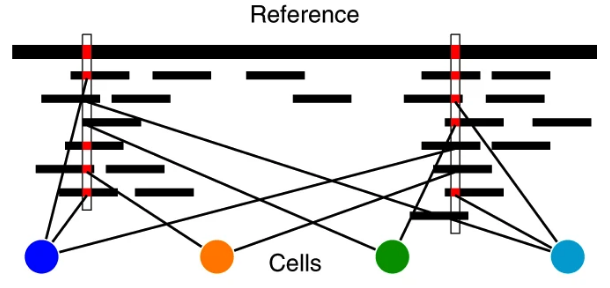
\includegraphics[width=0.3\textwidth, valign=c]{cellvariant.png} \label{fig:a}
}
\sidesubfloat[]{
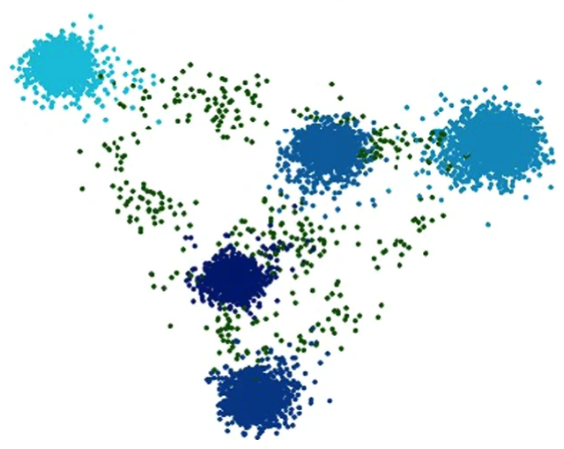
\includegraphics[width=0.3\textwidth, valign=c]{cellclust.png} \label{fig:b}
}
\sidesubfloat[]{
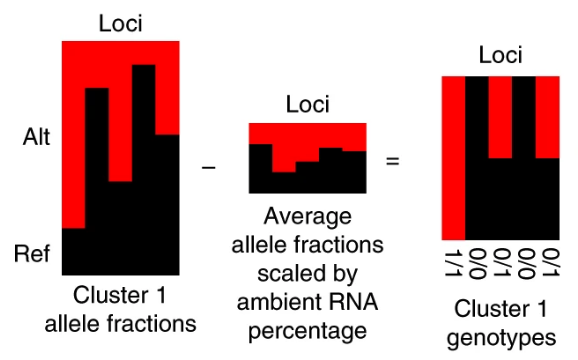
\includegraphics[width=0.3\textwidth, valign=c]{ambientrna.png} \label{fig:c}
}
\end{centering}
\floatfoot{\small{\textbf{a)} I find the variants in the reads from each cell barcode, \textbf{b)} cluster cells by their allele content and identify doublets, and \textbf{c)} use the bias in allele fraction from expected values to estimate and remove ambient RNA.}}

\end{figure}

\par{
In genome assembly, the goal is to use the overlapping read sequence similarity to infer that those reads came from the same locus in the genome and build contiguous sequences (contigs) that represent (in part or whole) the organism's chromosomes. The inference that these reads originated from the same genomic locus is complicated by repeats, heterozygosity, and sequencing errors. With inexact homology, one must disambiguate whether the differences arose from errors, paralogous repeat sequences, or from the alternate haplotype. If one cannot make this distinction and no reads span this region into unique sequence, the contig must be broken, resulting in a fragmented assembly. If the contig is not broken, one risks a chimeric misassembly of sequences that are distant to one another being assembled together. In chapter 3 I discuss the first high quality assembly of a single mosquito. Prior to this, DNA requirements for long read sequencing (discussed in section \ref{section:longreads}) were too high to extract enough high molecular weight (HMW) DNA from many small organisms including mosquitos. This required pooling multiple individuals together in order to meet the DNA requirements for these sequencing technologies. Pooling individuals increases the number of haplotypes in the extracted DNA and makes distinguishing repeat from heterozygosity harder. Through recent advances in library preparation, the DNA requirements for long reads has been greatly reduced. By sequencing a single mosquito with long reads, we reduce the number of haplotypes from many down to two thus decreasing the potential ambiguities that arise from heterozygosity. I then compare this genome assembly to the current gold standard assembly of \textit{Anopheles gambiae} that was created using bacterial artificial chromosome (BAC) Sanger sequencing (discussed in section \ref{section:sanger}), a dramatically higher cost method of creating high quality genome assemblies. We show many improvements in our assembly over the previous gold standard as well as highlight several issues that remain with the (then) current assembly state of the art.
} 



\par{
I continue to address the problem of heterozygosity in chapter 4 by showing several ways in which haplotype phasing consistency can be used as a signal for physical linkage. Given two or more proximate heterozygous loci, sequencing reads containing them should segregate into distinct groups according to which alleles they contain. But how do we know that a site is heterozygous? Initially we do not. We can find sequences which have inexact homology each being read roughly half (assuming diploid) of the times homozygous sequences occur. These could be due to heterozygosity or paralogous sequences (if both loci are under sampled by random chance). In both cases, reads containing multiple of these alleles should segregate into two (assuming copy number of the repeat is two) groups. But when comparing a true heterozygous site with an inexact homologous sequence caused by paralogous sequence, the reads with both alleles of the heterozygous site will contain one of the presumed alleles caused by the repeat sequence. We can use this property to avoid misassemblies, create phased assemblies, and scaffold contigs in a phasing aware fashion. In chapter 4, I outline how we identify \textit{de novo} candidate heterozygous sequences, define the phasing consistency criteria, build a phased assembly graph, and perform phasing aware scaffolding of contigs. If we wish to phasing aware scaffold an existing assembly, we must first phase its haplotypes. For this reason, I also provide an algorithm for haplotype phasing. This tool has the added benefit of being robust to being given non heterozygous sequences as input and can use the phasing inconsistency to correct those genotypes. I demonstrate these techniques on data from the butterfly \textit{Vanessa atalanta}.
} 

\begin{figure}[htbp!]
\begin{centering}

\caption{Phasing consistency as a \textit{de novo} signal for physical linkage}\label{fig:phasstools}
\sidesubfloat[]{
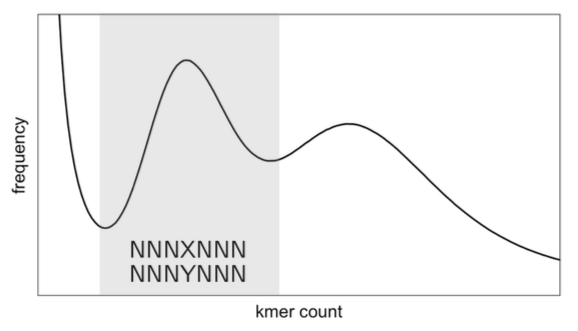
\includegraphics[width=0.3\textwidth, valign=c]{spectrum.png} \label{fig:a}
}
\sidesubfloat[]{
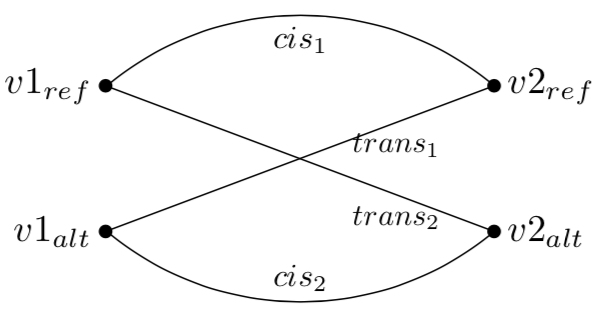
\includegraphics[width=0.3\textwidth, valign=c]{consistency2.png} \label{fig:b}
}
\sidesubfloat[]{
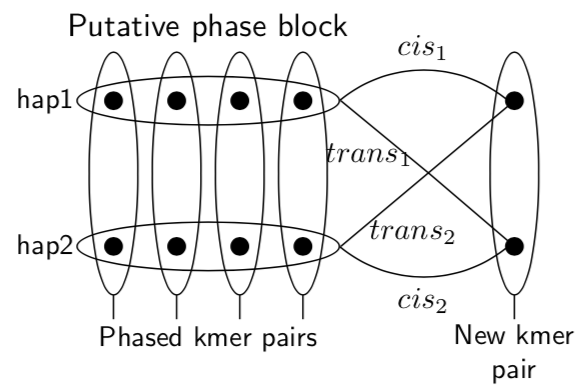
\includegraphics[width=0.3\textwidth, valign=c]{consistency3.png} \label{fig:c}
}
\end{centering}
\floatfoot{\small{\textbf{a)} We use the kmer count spectra to determine candidate heterozygous kmer pairs which we can then \textbf{b)} assess for phasing consistency based on the alleles on reads that contain one of each, and \textbf{c)} build a phased assembly graph.}}

\end{figure}

\par{
The remainder of this chapter contains the background and context for the work briefly described above. I first cover the history of single cell sequencing and analysis. I then outline the biases and errors that occur in single cell sequencing and the various solutions and their downsides which motivates chapter 2. I then cover a short history of DNA sequencing methods as well as assembly and scaffolding algorithms. I discuss the inherent ambiguities that can occur and the errors that can arise and their causes, which motivates chapters 3 and 4.
}

\section{Single Cell RNAseq}

\par{
The etymology of the word cell comes from the latin \textit{cella} meaning storeroom or chamber. These entities separate the physical space into compartments which interact selectively with their environments. This partitioning the cell provides is necessary for life due to the second law of thermodynamics and the nature of life. In Erwin Schrodinger's classic lecture series and book titled ``What is Life''\cite{whatislife}, he noted that while closed physical systems will always tend toward increased entropy (stated by the 2nd law of thermodynamics\cite{thermodynamics1}\cite{thermodynamics2}\cite{maxwell}), life must maintain (on average) a neutral or negative entropy\footnote{Incidentally, Erwin Schrodinger, as the father of quantum mechanics, along with Josiah Gibbs, as the father of statistical mechanics, will appear again later in this thesis as some of the algorithms described take ideas inspired by these fields for search strategies in optimization problems.} in the portion of the system in which it resides\cite{informationtheorylife}\cite{astrobiology}\cite{extremalities}. In order to do so, this requires the expenditure of energy. Biological evolution found an economical way of solving this problem with the bilipid membrane with various embedded molecules giving it the property of semipermeability---allowing some molecules in and not out or vice versa in a dynamic fashion. These cells proved, over time, to be so successful as to become the primary unit and building block of biological life on this planet. 
} 

\par{
When studying the state of a cell and its current function, we could try to measure many different properties such as the proteome, transcriptome, genome, chromatin accessability, environmental conditions (such as hormone content, pH, etc), cell surface proteins, etc. But we are somewhat limited by the tools available, and when addressing function, we first turn to the central dogma of molecular biology\cite{centraldogma} that states that information in general passes from DNA to RNA and then to proteins. If we could easily inspect the protein content of many cells in a high throughput fashion, that would be desirable, but protein detection and sequencing methods are often only limited to one or a few proteins at a time and/or are not high throughput\cite{immunohistochemistry}\cite{multiIHC}\cite{westernblot}\cite{western2}\cite{multimassspec}\cite{ionbeam}\cite{cellIHC}\cite{proteinsequencing}. But we do have a very high throughput detector for DNA and thus RNA by converting it to complementary DNA (cDNA) via reverse transcription.
}

\subsection{Bulk RNAseq}
\par{
Scientists have been sequencing cDNA libraries of RNA isolated from many cells mixed together since the advent of next generation DNA sequencing technologies (discussed in section \ref{section:nextgen}) became available\cite{RNAseq1}\cite{RNAseq2}. Because these use extractions from pools of cells, they are denoted as `bulk' RNAseq. These experiments have driven many biological discoveries, but for some applications their usefulness is limited because they represent the average transcriptome across a population of potentially diverse cells. This blurs the data and makes inference on minority cell types difficult if not impossible. The amount of RNA in a human single cell is roughly 10-30pg\cite{howmuchrna} that until recently was not enough to create a complex cDNA library even with amplification. Some researchers have isolated specific cell types using Fluorescence Activated Cell Sorting (FACS)\cite{FACspatent}\cite{FACs} prior to RNAseq with some success\cite{FACszebra}, but due to FACS cell stress and it only accessing one cell type at a time it was of limited utility.
}

\subsection{Single cell RNA sequencing}

\par{
In the past decade, technical advances in methods for the preparation of samples containing minuscule amounts of nucleic acids have made it possible to study the transcriptome of single cells\cite{first_singlecell}. This has changed the way biologists could access the functional state of individual cells within a complex and diverse population of cells in tissues across different states of organisms, shedding light on the cellular response to diseases, drugs, development, and more.
} 
\par{
There are many types of RNA in the cell including messenger RNA (mRNA), transfer RNA (tRNA), ribosomal RNA (rRNA), micro RNA, and small nucleolar RNA, and non coding RNA. mRNA makes up only 3-7\% of the cell's total RNA by mass\cite{rnacontent}, but it is what is translated by ribosomes into proteins, that conduct a large amount of the function of the cell. scRNAseq targeting other types of RNA have also been developed for alternative types of RNA for specific purposes\cite{nonmRNASC}, but in this thesis, scRNAseq is referring to a system that enriches for mRNA by using the 3' polyadenylation most mRNAs have (with some exceptions\cite{nonpoly}).
}

\subsection{Technologies}

\par{
mRNA from a single cell was first isolated and amplified to measurable levels with polymerase chain reaction (PCR)\cite{PCR}\cite{PCRPatent} in the early 1990s\cite{earliersinglecell} before the sequencing revolution. Without a high throughput detector, and due to the exponential nature of PCR causing abundant mRNA to dominate the sample, very few genes were detected. Detection improved with linear amplification achieved by multiple cycles of transcription of antisense RNA from the initial cDNA using T7 RNA polymerase\cite{T7amp} and the advent of oligonucleotide microarrays\cite{snpchip} allowing for RNA microarray studies detecting over a thousand genes\cite{microarrayRNA}\cite{microarraySC2}. However, the number of genes measured were still a fraction of the total genes expressed. The first sequencing of single cell cDNA sequencing increased the number of genes detected by 75\%\cite{first_singlecell} and provided a hypothesis free measurement of the transcriptome a single cell. Since then, scRNAseq has grown greatly in the number of cells processed per experiment, the number of genes detected per cell, and its uptake by the scientific community\cite{singlecellgrowth}.
}

\par{
Current scRNAseq protocols convert RNA to cDNA using a reverse transcriptase primed off of the poly-A tail of the mRNA. In this process, a cellular barcode oligo as well as template switching oligo (for subsequent PCR) are added to the construct. Often, a unique molecular identifier (UMI) is also added. This is used to determine which cDNA molecules were amplified from the same RNA source molecule to avoid counting PCR duplicates multiple times\cite{UMI1}\cite{UMI2}.
} 

\par{
To deliver a barcode oligo to all of the reads originating from one cell and different barcodes to different cells, physical separation of one form or another is generally used. The separation could be in different tubes, plate wells, nanowells\cite{seqwell}\cite{scalablemicro}\cite{combilabel}, or more recently with microfluidic systems creating reverse emulsion droplets\cite{dropseq}\cite{Klein2015}\cite{10xsinglecell}. These methods vary in several parameters including the scalability of number of cells per experiment, the mRNA capture rate, and the technical variation between experiments among others\cite{powersingle}\cite{singlecompare}\cite{singlecompare2}. Which method is best to use ultimately depends on the biological question. For experiments where sampling the whole population of cells is important, droplet and nanowell methods are better whereas if capture rate and amount of data per cell is paramount, plate based systems might be more appropriate. 
}

\subsubsection{10x Genomics}

\par{
In this thesis, all of the single cell data presented was generated using the 10x Genomics Chromium platform, a reverse emulsion droplet based system. Figure \ref{figure:10xsinglecell} outlines how this system works. It uses a microfluidic system to deliver gel beads, reagents, and cells into reverse emulsion droplets where the reverse transcription occurs. The gel bead contains a construct with the cell barcode oligo, a UMI, and adapters for Illumina sequencing\cite{10xsinglecell}\footnote{I was fortunate to have worked at 10x Genomics between 2014 and 2017. While I did not work much directly on the single cell technology (I primarily worked on the company's first product, linked reads), I gained much insight into the data by being present for its creation.}.
}
\begin{figure}[htbp!]
\caption{10x Genomics single cell RNAseq}
\label{figure:10xsinglecell}
\begin{centering}
\sidesubfloat[]{
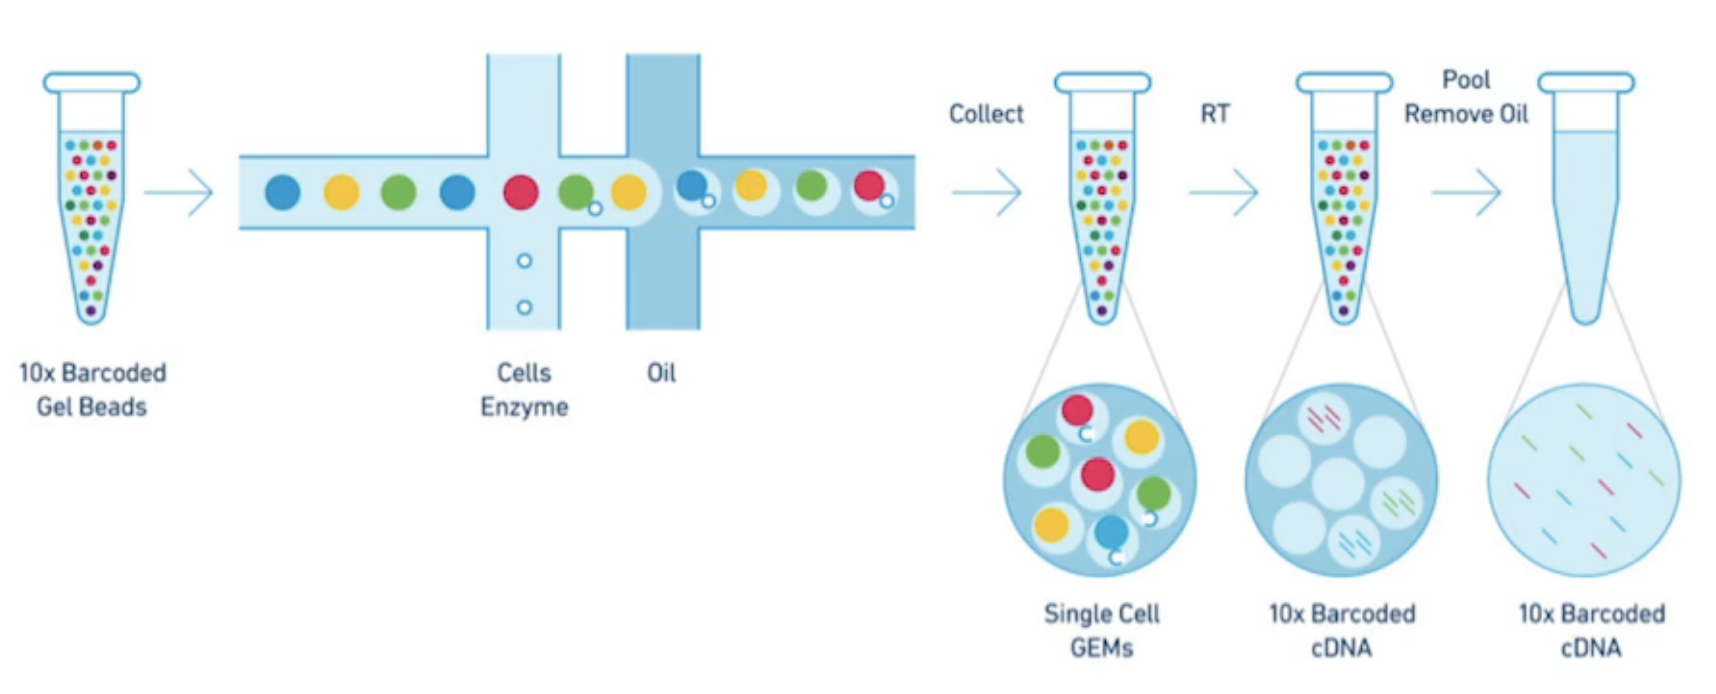
\includegraphics[width=0.85\textwidth]{singlecelloverview2.png}} \\
\sidesubfloat[]{
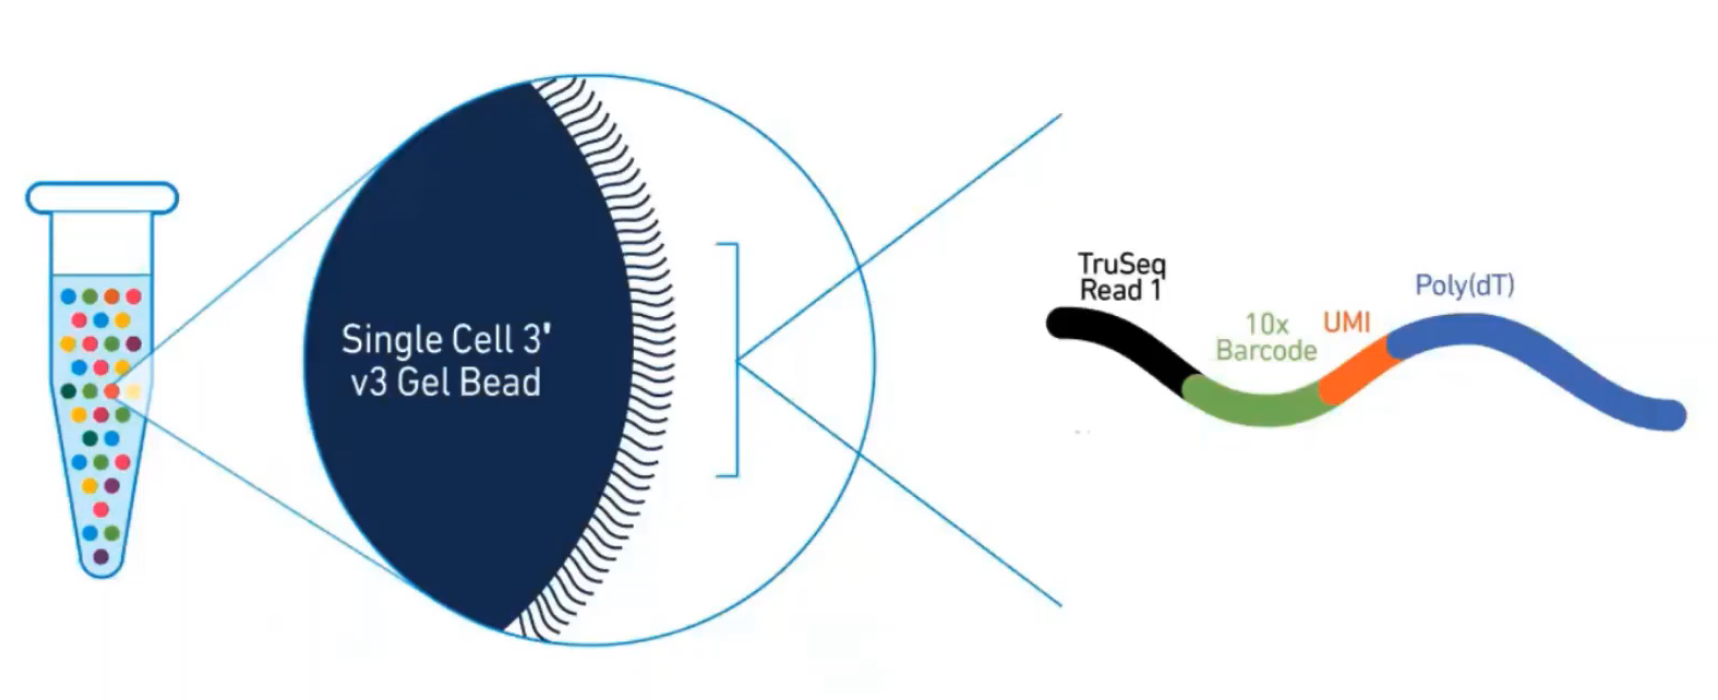
\includegraphics[width=0.85\textwidth]{singlecell2.png}
}
\end{centering}
\floatfoot{\small{Diagram outlining 10x Genomics single cell sequencing technology (image credit: 10x Genomics website\cite{10xwebsite}).}}

\end{figure}

\subsection{Analysis of scRNAseq data}

\par{
This construct is then sequenced on a next generation Illumina sequencer \cite{bridgeamp}\cite{illuminareview} (discussed in detail in section \ref{section:nextgen}) giving paired-end reads with one read containing the cell barcode and UMI and the other read containing the cDNA of the mRNA transcript. Other sequencing platforms have been used, notably long read sequencing platforms, to get the whole transcript read to investigate alternative isoforms, but will not be discussed further here\cite{tilgner}\cite{isoformseq}\cite{longreadsinglecell}. The most common software package used to produce cell by genes expression counts matrix and initial cell type clustering is cellranger\cite{cellranger} and while alternatives exist\cite{dropseqsoft}, they do largely the same steps. 
}

\subsubsection{Genome alignment}

\par{
First, the template switch oligo and polyadenylation are trimmed from the 5' and 3' ends of read two respectively. Then the read two is mapped to the given reference genome using the STAR splicing aware RNA aligner\cite{STAR}. Other aligners exist for this purpose such as HISAT2 \cite{hisat} and TopHat2 \cite{tophat2}. Also there are psuedo-aligners (Kallisto\cite{kallisto} and Salmon\cite{salmon}) which are much faster and robust to sequencing errors but do not provide base level alignments\cite{alignfree}. The reads are then marked as exonic or intronic using the given transcript annotation gene transfer format (GTF) file and confident or not based on if the read overlaps an exon for >50\% of its length and if the mapping quality (mapq) is 255 which indicates that the read aligned uniquely. Confident exonic reads are carried forward to the UMI counting step\cite{singlecelloverview}.
}

\subsubsection{Barcode correction}
\par{
Before counting UMIs, cellranger attempts to do barcode correction on the cell barcodes. 10x Genomics uses a designed barcode set of either 737k or 3m barcodes each with a hamming distance\cite{hamming} of at least two to any other barcode in the set. The barcodes that make up this designed set are the barcodes we expect to see and this set is termed the whitelist. In order to error correct barcodes, first the frequency of each barcode in the whitelist is counted. Then for every barcode that is not in the whitelist, each barcode that is one hamming distance from this sequence and is on the whitelist is found. A posterior probability is computed with the priors set by the frequency of that whitelist barcode and the base quality of the changed base used to determine likelihood of that error. For a barcode correction to then take place, the posterior probability of that whitelist barcode must be over 97.5\%\cite{barcodecorrection}.
}

\subsubsection{UMI counting}

\par{
PCR duplicates are then removed. If any reads have cell barcode, gene, and UMI, all are removed except one. The remaining reads will be counted to create the cell barcode by gene count matrix. 
}



\subsubsection{Cell-barcode detection}
\par{
Note that not each cell barcode contains a cell. Due to ambient RNA in solution from cells lysed before reverse emulsion partitioning, droplets without an intact cell will have some reads. We next need to determine which cell barcodes have cells and which do not. Initially, droplets containing cells were called using the second derivative of the log-log UMI counts by barcodes plot (see figure \ref{figure:knee}). More recently, a method using the RNA content of the confidently empty droplets called EmptyDrops\cite{emptydrops} was developed to compare that RNA content (which is generally an average of the RNA content of all cells assuming each cell type lyses with equal probability) with the RNA content of the cells to determine an appropriate cutoff where the transcription profile from the average is dramatically different. This particularly helps in situations where the sample contains some cells with a large amount of transcripts and another cell type with many fewer transcripts. Both of these cell types will likely still have a very different transcriptional profile than the empty droplets. This algorithm has now been implemented in cellranger. The raw cell barcode by genes UMI counts matrix is then filtered to retain only cell containing cell barcodes.
}

\begin{figure}[htbp!]
\caption{Cell barcode detection knee plot old vs new algorithm}
\label{figure:knee}
\begin{centering}
\sidesubfloat[]{
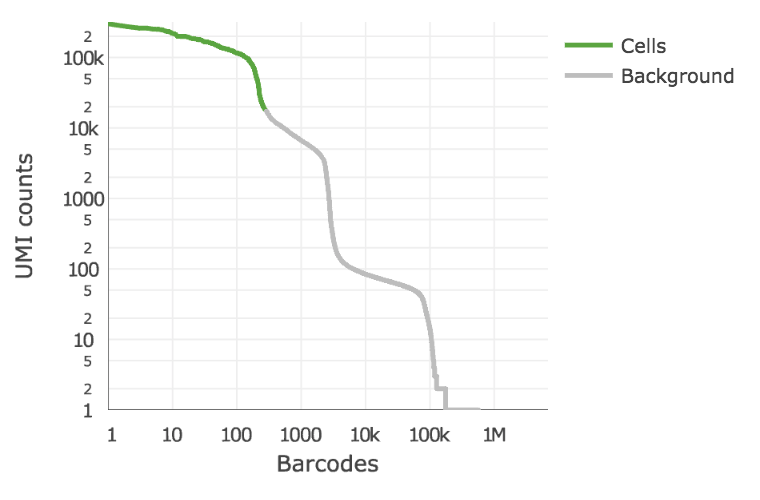
\includegraphics[width=0.45\textwidth]{knee1.png}} 
\sidesubfloat[]{
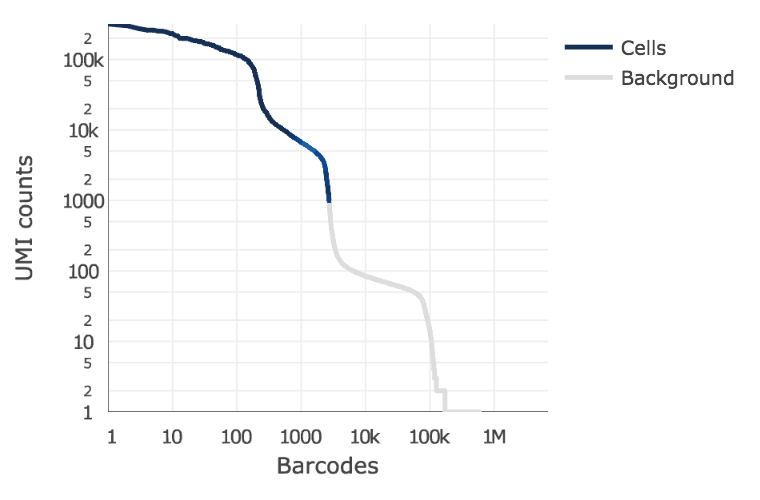
\includegraphics[width=0.45\textwidth]{knee2.png}
}
\end{centering}
\floatfoot{\small{Log-log barcode by UMI count knee plots showing which barcodes were determined to contain cells under the \textbf{a)} old method using 2nd derivative and the \textbf{b)} new EmptyDrops method (image credit: 10x genomics website\cite{10xwebsite}).}}

\end{figure}

\subsubsection{Quality control}

\par{
Many of the following steps are done in software packages downstream from cellranger that aim to implement many types of analyses for scRNAseq data. The most popular of these software packages is Seurat\cite{seurat1}\cite{seurat2} and while alternatives such as Monocle\cite{monocle} exist, a comparison is out of the scope of this thesis.
} 

\par{ In the process of cell dissociation, liquid handling, and partitioning, some cells may be damaged. For this reason, many researchers use different criteria to remove these poor quality cells. Some also use different criteria for different cell types and so a less stringent global filter may be applied prior to cell type detection and further filtering. These criteria include the number of genes per cell, percent mapped reads, percent reads that map to spike in controls, percent mitochondrial reads, and percent of reads that are PCR duplicates. While these are reasonable markers for dead or dying cells\cite{osorio}\cite{ilicic}, it is my personal opinion that this type of quality control should be limited and determined at the experimental design stage to prevent unintentional bias in the results due to how these thresholds are chosen. Of course, there will always be a trade-off between unbiased data and clean data for downstream analysis and each application may require differing levels of quality control.
}

\subsubsection{Normalization}\label{section:normalize}

\par{
As previously discussed, individual cells have extremely small amounts of mRNA and require methods to amplify this material in order to be made into a cDNA library and sequenced. These methods, along with the innate difficulties of measuring such a small amount of starting material inevitably result in some technical artifacts. Genes that are expressed to a lesser degree than other genes may show zero counts or lower than true counts in the experiment for several reasons\cite{technoise}. Capture rate of mRNA in the reverse transcription step will never have complete yield and may vary from cell to cell and gene to gene. Additionally, genes that are expressed might be made into cDNA and amplified, but not sampled in the sequencing step as transcripts that begin with a higher copy number get amplified more in the exponential PCR step. Differences in cell size, and thus mRNA content, may result in sampling of genes in one cell type not sampled in other cell types even if both express them. To address this, many normalization methods have been developed\cite{normalize1}\cite{normalize2}. Spike in controls can be used to improve this normalization\cite{marioni1} but takes up valuable sequencing. Another solution is imputation\cite{imputesc}, but this can introduce unwanted false positives\cite{fpimpute}. In comparison papers, differential expression analysis has been shown to be the downstream application most sensitive to these methods\cite{normalsc}, with scran\cite{scran} performing the best of those tested.
}

\subsubsection{Visualization}

\par{
In order to visualize this high dimensionality data, we must project it into two or three dimensions in a way that preserves the biologically interesting structure at multiple scales. First, a principal component analysis (PCA) of the filtered cell by gene counts is done to find the most meaningful features and reduce the dimensionality from cells by genes to cells by $M$ where $M$ is a user settable value\cite{pcaimpl}. For most experiments, the complexity of the transcriptional profile cannot be easily gleaned by looking at the first two-three principal components visually, so the next step is to use non-linear dimensionality reduction techniques to bring the data into a visually informative two or three dimensional space. The two most popular methods for this are the t-Stochastic Neighbor embedding (t-SNE)\cite{tsne1}\cite{tsne2}\cite{hinton} and the Uniform Manifold Approximation and Projection (UMAP)\cite{umap1}. Both of these methods aim to preserve pairwise distances in the final projections, but are parametric and non-deterministic (without a fixed psuedorandom number generator seed). There is an inherent trade-off between how well distances should be preserved at different scales, which the parameters can help guide. However, due to the randomness and parametric nature of these algorithms, it can lead some researchers to use them to bias the results toward the expected outcome of their hypothesis. Nonetheless, these are powerful techniques to understand highly dimensional data such as single cell RNAseq. Recently, UMAP has grown in popularity over t-SNE because it has been shown to better preserve pairwise distance due to the improved initialization strategy employed in the primary implementation and is more computationally efficient than t-SNE\cite{umap2}\cite{umap3}. These projections are often fed into downstream analysis such as clustering and lineage reconstruction. It is not clear that clustering in this space is better than clustering on the raw data, PCA, random projection\cite{randomproject}, or other dimensionality reduction space, but they are likely to look more visually correct in the UMAP or t-SNE space when both the clustering and visualization is in the same projection. An analysis of this observation is out of the scope of this thesis.
}


\subsubsection{Cell type clustering and annotation}

\par{
It is useful to group similar cells together for the purposes of cell type annotation and cell state detection. Because individual cells may not have enough UMIs sequenced, these analyses may not be possible on an individual cell basis whereas grouping similar cells together will pool enough data to conclusively do so. Clustering is typically done on the dimensionality reduced data (either PCA or UMAP/t-SNE) and many methods have been used including K-means, hierarchical clustering, graph based methods and meta-heuristics have been applied including consensus clustering, cluster trees among others\cite{scclustreview}\cite{subpop}\cite{sc3}\cite{clustree}. These methods are reviewed in \cite{scclustreview} and otherwise a comparison of these methods is out of the scope of this thesis.
} 

\par{
Once cells have been clustered into similar groups, we can try to understand what each of these groups of cells represent. Marker genes have been studied for many decades to identify and differentiate different cell types. One can visually display the expression values of these marker genes versus the cell clusters to find the cell types of interest. Increasingly more popular are automatic methods which use annotated cell atlases to match cell types. These include scMatch\cite{scMatch}, cellHarmony\cite{cellHarmony}, Garnet\cite{Garnet}, scPred\cite{scPred} with some using prior knowledge of marker genes and some not. A comparison of these methods found that they work fairly similarly with scPred performing the best overall. Interestingly, they find that prior knowledge of marker genes does not improve performance. Other methods allow you to project cells from one dataset onto another\cite{scmap}. For systems which have robust prior annotated datasets, these are powerful and accurate tools for automatic annotation.
}



\subsection{Downstream analysis}
\par{
Many further analyses on single cell experiments are possible and a comprehensive review of these is out of the scope of this thesis. Pseudotime analysis can order cells along some cell state change such as differentiation or cell cycle\cite{pseudotime}\cite{scHOT}. Gene regulatory networks may be inferred using the correlation of genes indicating they may be under similar regulatory control\cite{scenic}. Somatic mutations in the mitochondrial genes can be used to discover cell lineages\cite{lineage}. And many more analyses are possible especially if the experimental design is non-standard such as multi-Omic single cell sequencing or CRSPR-Cas9 screening\cite{perturb} is added to the mix.
}

\subsection{scRNAseq error modes}\label{section:scerrors}

\subsubsection{Batch effects}

\par{
Due to the manner in which scRNAseq data is created, it naturally has certain noise and error characteristics. In section \ref{section:normalize}, we discussed intra-dataset technical artifacts. Naturally, inter-dataset technical artifacts are larger in magnitude and more diverse. If any of the laboratory protocols were changed, or the experiment was done by a different person, on a different day, at a different temperature, it may introduce inter-dataset differences that may be even larger than the biological differences we wish to measure. There are a multitude of computational methods to correct these batch effects such as scanorama\cite{scanorama}, mnnCorrect\cite{batch1}, BBKNN\cite{BBKNN}, Harmony\cite{harmony}, Seurat\cite{seurat3}, and LIGER\cite{LIGER}. Each of these either finds matching cell populations or overall data correlations to then create a projection to bring the datasets into a common space. A comparison study tested 14 of these methods and evaluate the adjusted rand index of cell type clustering, average silhouette width of cell type clustering, and two other metrics and found that Seurat, LIGER, and Harmony performed best. While these are powerful tools for correcting these technical variations, it is possible that in trying to correct for variation due to batch effects that some biological differences will also be erased or biased.
}

\subsubsection{Doublets}

\par{
In 10x Genomics scRNAseq, the loading of droplets with cells is a random process that follows a Poisson sampling distribution. The experiments are designed with a cell suspension concentration to produce a poisson distribution with a mean much less than one. This results in an experiment in which most droplets sample zero cells and some sample one cell. But in order to collect enough cells, that mean still must not be vanishingly small. So some droplets will sample more than one cell. These cell barcodes associated with more than one cell are generally called doublets though multiplets might be more appropriate as some may have more than two cells. Another way that these arise is if the tissue dissociation of cells was not complete or if there is any cell adhesion causing cells to travel together in suspension. Again, a number of computational tools have been developed to find and remove these doublet cell barcodes from further analysis. These include doubletCells\cite{doubletCells}, DoubletFinder\cite{doubletfinder}, Scrublet\cite{scrublet}, DoubletDecon\cite{doubletdecon}, scDblFinder\cite{scDblFinder}, and Solo\cite{solo} among others. Many of these use simulated doublets by combining \textit{in silico} the UMI counts of putative singleton cells to identify what the transcriptional profile of a doublet would look like. Validating these methods is somewhat problematic as in real datasets, the doublets are not known, and simulated doublets may not exactly match what data would look like from true doublets. In a recent benchmark of these methods, many of these performed similarly with scDblFinder scoring the highest overall\cite{doubletbench}. Once again, these are powerful methods, but do not work flawlessly and in particular may remove cells in an intermediate state transition between two more distinct cell types in the sample so may remove cells of potential interest.
}


\subsubsection{Ambient RNA}

\par{
Another aspect of scRNAseq data that biases our view of the transcriptional landscape is ambient RNA. Before the cells are partitioned, some cells may have lysed, or there may be other cell free RNA in solution. This RNA will be delivered to all droplets including droplets that contain a cell and that RNA will be sequenced with the same cell barcode as the reads that truly came from the cell. This is alternately called ambient RNA or the `soup'. Ambient RNA can be analyzed by looking at the reads from non-cell barcodes and is generally an average of all of the RNA in the experiment, but this is not always true such as when some cell types are more prone to lysing than others or samples such as necrotic tumor. The amount of ambient RNA in the system is generally small, but may be increased in some samples such as tissues that requires harsh detergent agents to dissociate the cells into a cell suspension. SoupX was developed in order to estimate the amount of ambient RNA and remove it\cite{soupx}, but requires prior knowledge of gene expression in different cell types as it uses measurement of genes known to not be expressed in certain cell types to measure the ambient RNA. 
}

\subsubsection{Mixtures}

\par{
One experimental design that promises to solve all three of these error modes in scRNAseq are mixture experiments. If cells from multiple samples are mixed together, you limit the number of technical artifacts between them to differences in how the cells were treated prior to being mixed. If you can distinguish which cells came from which samples, you can use that same signal to determine which cell barcodes represent cross-sample doublets. And depending on the sample features, this may also aid in measuring ambient RNA. Several experimental methods have been developed to tag cells by sample prior to mixing. Cell hashing uses oligonucleotide tagged antibodies attached to cell surface proteins as a sample signal\cite{cellhashing}\cite{nucleimulti}. MULTI-seq uses lipid and cholesterol modified oligonucleotides which incorporate into any lipid membrane to generate a sample read-out\cite{multiseq}. CellTag uses heritable genetic material as a sample index for tracking cells through passages after mixing to better study sample interactions\cite{celltag}. These are powerful methods for reducing batch effects, detecting doublets, and reducing costs through both multiplexing and giving more scope for overloading the number of cells per experiment. As the number of cells per experiment is increased, the number of doublets grows as well. If one has a robust method of identifying and removing doublets, one can load more cells and recover more singletons even after removing the doublets. However, there is a limit to this. 10x Genomics reports that the number of doublets is roughly 1\% per thousand cells recovered. This is of course an oversimplification. If the cell suspension is fully dissociated, the cell loading is a Poisson process. In the range of two to ten thousand cells, this generates roughly 1\% doublets per thousand cells. Outside of this range, this rule falls apart. One can, however, fit a Poisson to a number of different experiments with differing number of cells for a better model. Over some number, the marginal increase in singletons recovered as more cells are added decreases and at some point actually diminishes. This is also worsened by the fact that the doublets and multiplets take up valuable sequencing only to be discarded. Additionally, doublet detection methods are not perfect and the remaining doublets will bias your experimental results. 
} 

\par{
But these methods require additional experimental work and are not always possible. Some mixture samples are naturally occurring such as at the maternal/fetal boundary, transplant patient tissue, or complex infections. If the mixed samples have distinct genotypes, one can use the genetic variation between samples to demultiplex them. Demuxlet was first developed for this purpose, but requires prior knowledge of the genotypes of each sample and its rigid model based system can make errors especially as the amount of ambient RNA in the system increases\cite{muxseq}\cite{demuxlet}. In chapter 2, I present souporcell, a method for clustering cells by genotype without prior knowledge of each sample, cross sample doublet detection, and ambient RNA measurement. We compare our system against Demuxlet and two other methods, scSplit and vireo\cite{scsplit}\cite{vireo}, across a wide range of challenging datasets. Since then, freemuxlet was developed as another such method, but is not compared to as it came out later and is unpublished outside of a thesis\cite{freemuxlet}.
}

\section{Genome assembly and scaffolding}
\par{
Since Mendel's discovery of the laws of heritability\cite{mendel}, it has been a goal to link the micro to the macro to explain evolution in a quantitative fashion\cite{evolutionmicro}. The discovery that DNA encoded the hereditary information of organisms\cite{Avery} and subsequent discovery of its chemical structure\cite{watsoncrick} made clear the nature of information storage in a linear polymer and mechanism for stable replication. Even before the discovery of mRNA\cite{mRNA1}\cite{mRNA2}, Francis Crick hypothesized that nucleic acids direct the synthesis of proteins\cite{proteinsynthesis} and later elucidated what is now known as the central dogma of molecular biology\cite{centraldogma1}. In brief, this states that the information flow of an organism is through the DNA being transcribed into RNA and the RNA translated into proteins which perform most of the functions of the cell. With the information source being the DNA, this made clear the importance of reading the sequence. And for several decades, our ability to read DNA sequence has dramatically increased in both amount and accuracy.
}

\subsection{DNA sequencing}

\par{
The history of DNA sequencing is generally thought of as having three waves---Sanger sequencing, next generation sequencing, and third generation sequencing. Sanger sequencing is highly accurate and produces relatively long reads at 500bp to 1kb but is not highly scalable. Next generation sequencing produces high accuracy short reads (initially 35bp, but now can be up to 250bp) and is massively scalable. At the same time, many other sequencing technologies came along without much success. In the third wave, the ability to sequence long reads of single molecules without amplification has transformed genome assembly. PacBio and Oxford Nanopore Technologies (ONT) developed single molecule long read sequencers that produced low accuracy (85\% and $\approx$90\% respectively) long reads limited mostly by the input DNA length and stability. More recently, PacBio utilizes circular consensus sequencing (CCS) to produce reads in the 5-25kb range with high accuracy. Due to the vast differences in application performance long accurate reads bring, it could be argued that this represents the fourth generation of DNA sequencing.
}

\subsubsection{Sanger sequencing}\label{section:sanger}

\par{
The ability to sequence proteins and certain RNA molecules came before the ability to sequence DNA due to proteins being made of more diverse monomers and RNA not being complicated by a complementary strand\cite{aminoacidsequence}\cite{sequenceofsequencers}. In 1965, Robert Holly and Frederick Sanger developed two related methods for sequencing RNA\cite{Holly1}\cite{Sanger1}. These were labor intensive and Sanger's method employed dangerous radioactive material. This method was then extended to DNA in 1973 and used to sequence 50 bases of the phage f1\cite{Sanger2}. Eventually, the use of polyacrylamide gel electrophoresis, chain termination chemistry with dideoxynucleotides, the use of flourescence instead of radiolabeling, and automation brought us to what is know known as Sanger sequencing\cite{Sanger3}. This technology was automated and became the most popular method of sequencing for many years\cite{Hunkapiller1991}. These sequences are highly accurate as each base signal is the result of the termination of a many molecules and have read lengths from 500bp to 1000bp which is limited by reaction efficiency requiring a fraction of chain terminations at every base of the sequence. This method requires clonal DNA and thus laboratory methods were developed for creating libraries for sequencing. BACs and YACs \cite{BACsYACs} were developed and each end could be sequenced creating a mate pair read spanning hundred of kilobases giving long genetic distance linking information.
}

\subsubsection{Short reads}\label{section:nextgen}

\par{
In the poorly named ``next generation'' phase of DNA sequencing, there were many technologies created, but ultimately one became the dominant one and discussing each in detail is out of the scope of this thesis. In the late 90s, Solexa (later acquired by Illumina) created the Genome Analyzer in which DNA attaches to a primer on a flow cell surface and is amplified into clonal arrays of single stranded DNA\cite{flowcell}. This is achieved by what is known as bridge amplification. The DNA has two different primers attached during library preparation that correspond to two oligos on the flow cell. Initially, a polymerase creates the reverse strand and the double stranded DNA is denatured and the forward strand is washed way. The reverse strand then bends over (aka bridges) to attach to both oligos and the forward strand is synthesized. This bridge is then denatured resulting in forward and reverse single strands attached to the flow cell. This is then repeated multiple times and in the end one of the oligos on the flow cell is cleaved and those strands are washed away leaving many copies of only one strand of the DNA\cite{bridgeamp}. Fluorescently labeled dNTP are added and each DNA colony is then imaged. The terminator group is then removed\cite{reversibleterminator} and the process is repeated for each base. Because this method uses the synthesis of the second strand as the mechanism for sequencing, it is often referred to as `sequencing by synthesis'. 
} 

\par{
Initially the read length was limited to 35bp but over the years this has increased to 150bp on the high throughput sequencers and 250bp on the lower throughput MiSeq. The read length is limited by reagent stability as well as phase problems. If not every molecule gets extended at every step, eventually the signal will degrade until eventually it is impossible to tell which base is the correct one. Despite the short read length, paired-end reads are made possible by having a longer DNA insert than the read length and after reading one end, bridging the DNA on the flowcell and sequencing the other end. This technology produces highly accurate reads at roughly 0.1\% error rate. While many other sequencing technologies emerged in the same time frame, Illumina's was much higher throughput and was highly accurate and has few context specific errors when compared with the others\cite{errormotifs}. Illumina sequencing has made up the vast majority of DNA sequencing to this day, but other third generation technologies are increasing in utilization.
} 

\par{
Several methods build on next generation sequencing to add further information. Moleculo\cite{moleculo}, contiguity preserving sequencing (cpt-seq)\cite{cptseq}, long fragment read (LFR)\cite{LFR}, 10x Genomics linked reads\cite{10xlinked}, and more recently haplotagging\cite{haplotagging} use various methods for making short reads from long molecules and tagging each short read with a barcode specific to the HMW DNA molecule of origin. Strand-seq uses bromodeoxyuridine labeled DNA to degrade one strand of DNA which can be useful for haplotype phasing\cite{strandseq}\cite{strandseq5}\cite{strandseq2}\cite{strandseq3}. In chapter 4, I use 10x Genomics linked reads which I outline in detail in section \ref{section:linkedreads}.  
}

\subsubsection{High throughput chromatin conformation capture (Hi-C)}\label{section:hic}

\par{
Hi-C crosslinks cells' DNA with formaldehyde, breaks the DNA with a restriction enzyme, and blunt end ligation is used in conditions which prefer joining cross-linked DNA\cite{hic1}\cite{hic2}\cite{hic3}\cite{hic4}. This produces read pairs which were spatially close in the nucleus but may be far apart in the genome. Because of the 3D structure of the tightly wrapped genome in the nucleus, this means that most links are intra-chromosomal and thus is useful in assembly scaffolding\cite{SALSA}. Hi-C data is used extensively in chapter 4 for haplotype phasing and phasing aware scaffolding.
}


\subsubsection{Linked reads}\label{section:linkedreads}

\par{
The 10x platform for linked reads uses the same microfluidic system as in scRNAseq. Instead of delivering cells to the droplets, the linked read system delivers HMW DNA from which short reads are created. Whereas the barcode oligo acted as a cellular barcode in scRNAseq, it acts as a long molecule barcode in the linked read system. It starts with high molecular weight DNA input into a microfluidic system that partitions those long DNA molecules into GEMs (Gel bead in EMulsion) with oil surrounding an aqueous solution containing the DNA and reagents with a gel bead housing millions of copies of an oligo containing random primers, Illumina adapters, and the same barcode DNA sequence. Each different gel bead has a different barcode DNA sequence with high probability. Each GEM is Poisson loaded with HMW DNA and on average gets roughly ten long molecules in the standard workflow. Short sequences are then amplified from these long molecules with random priming, creating a construct with the Illumina P5 and P7 adapters, the barcode oligo, and the DNA insert. This is then sequenced using standard short read Illumina sequencing. All of the reads with the same barcode sequence come from the same GEM and thus from a handful of long molecules. When the reads are mapped to a reference genome, the reads from each barcode cluster into a few small regions of the genome associated with their molecule of origin. This long range information can then be used to map into repeat regions of the genome, phase haplotypes, and call structural variation\cite{10xlinked}\footnote{From 2014 to 2017 I worked at 10x Genomics and was the main developer on Lariat, the software used to confidently map into repeat regions of the genome, and had a role in the phasing algorithm including its ability to correct genotypes as well as on the development of the technology as a whole. I am grateful to have been a part of such a talented group of people and to have had the opportunity to learn from them.}.
}

\begin{figure}[htbp!]

\caption{10x Genomics linked reads}
\label{figure:linkedreads}
\begin{centering}
\sidesubfloat[]{
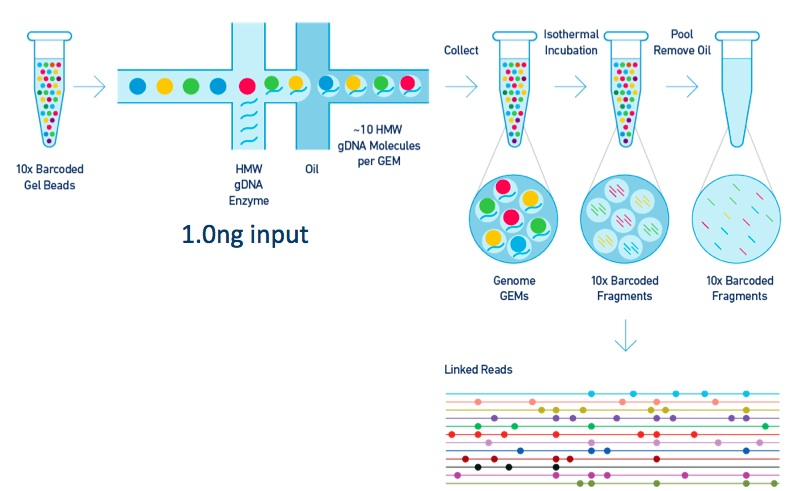
\includegraphics[width=0.65\textwidth]{linkedreads.jpeg} \label{fig:a}
} \\
\sidesubfloat[]{
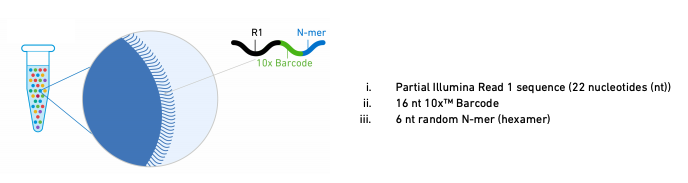
\includegraphics[width=0.65\textwidth]{gem.png} \label{fig:b}
} \\
\sidesubfloat[]{
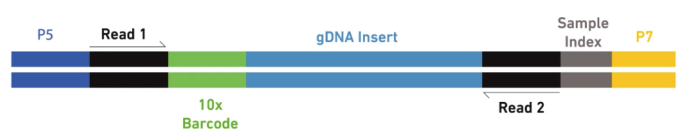
\includegraphics[width=0.65\textwidth]{construct.png} \label{fig:c}
}
\end{centering}
\floatfoot{\small{\textbf{a)} outlines the microfluidic system to create the Gel bead in reverse emulsion. \textbf{b)} shows the gel bead oligo setup and \textbf{c)} diagrams the final construct. (image credits to 10xgenomics website)}}

\end{figure}

\par{
While 10x Genomics Linked reads are used in Chapter 4 for phasing and phased assembly, the technology is no longer offered by the company. More recently, bead based systems have been developed that do not require a microfluidic system. In solution with microbeads, long DNA molecules tend to wrap around a single bead\cite{beadphasing}\cite{LFR}. Separately, Tn5 transposase has been used to insert adapter and barcode sequences at high frequency into genomic DNA\cite{cptseq}. With these ideas combined, Frank Chan's group has developed a technique called Haplotagging that uses microbeads bound to Tn5 transposase with one of 85 million molecular barcodes and Illumina sequencing adapters creating linked read libraries for a fraction of the price in a single tube\cite{haplotagging}.
}

\subsection{Third generation sequencing: long reads}\label{section:longreads}

\subsubsection{PacBio}

\par{
Pacific Biosciences (PacBio) uses microscopic wells known as zero-mode waveguides (ZMWs) along with single molecules of DNA and DNA polymerase, and optically measures fluorescent tagged nucleotides as they are incorporated by the polymerase. This is known as single molecule real-time sequencing (SMRT sequencing). The DNA template is ligated with hairpin adapter sequences known as the SMRTbell adapters to create a topologically circular template. This allows for multiple passes of the same DNA molecule. Initially, polymerase nucleotide incorporation and optical measurement speed were limited. That combined with the rate at which DNA polymerase dissociates from the molecule limited the number of times long molecules could be sequenced to once or just a few times. This results in long, but noisy reads with roughly 15\% error rate\cite{pacbio}\cite{blasr}\cite{clrerror} known as continuous long reads (CLR). The PacBio data used in Chapter 3 is CLR data. More recently, advances in the speed of polymerase nucleotide incorporation and optical measurements have allowed for many passes of the same long molecules. This allows for circular consensus sequence calling across these multiple passes creating High Fidelity (HiFi) reads with much higher accuracy ($<<$1\% error rate on average) while maintaining true single molecule sequencing\cite{HIFI}. Over the past few years, PacBio data---both CLR and CCS---has revolutionized genome assembly and is now used routinely for generating high quality reference genome assemblies\footnote{While I would take no credit for HiFi technology, it is poorly known the contribution that my good friend Brendan Galvin had on it. I don't know the full history, but when Brendan was working for PacBio in late 2017, he called me and offered three options for possible improvements to long read sequencing. Among these was longer read CCS data---he estimated the possibility of 10kb CCS reads. He asked me among his three options, which one would have the biggest impact on genome assembly. I responded that 10kb accurate reads would revolutionize the world of assembly. Within a year and a half of that conversation, this became a reality. Of course this was not entirely Brendan's doing either, but between his technical contributions and internal advocation for the technology, I am convinced he played a large role. This is just one of several major contributions to the field he has had.}. In chapter 4, I use PacBio HiFi data for phased assembly.
}

\begin{figure}[htbp!]
\caption{Circular consensus sequencing}
\label{figure:ccs}
\begin{centering}
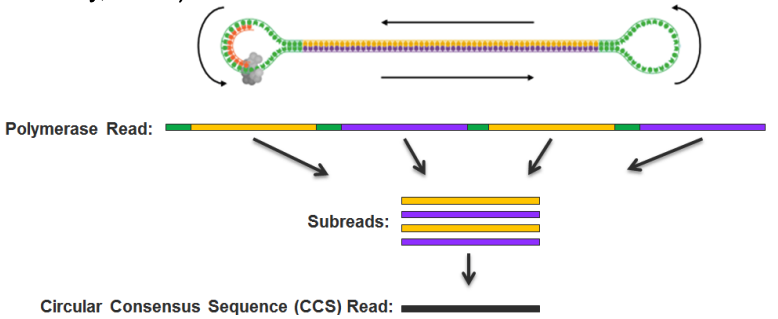
\includegraphics[width=0.65\textwidth]{CCS.png}
\end{centering}
\floatfoot{\small{Diagram outlining circular consensus sequencing (image credit: PacBio website\cite{PBwebsite}).}}

\end{figure}

\subsubsection{Nanopore sequencing}

\par{
The idea of reading single molecules of DNA by the current changes as a molecule translocates through a protein nanopore in a bilipid membrane by electrophoresis goes back to the 1980s\cite{nanopore1} but took twenty-five years of work before Oxford Nanopore brought the technology to market\cite{nanopore2}\cite{nanopore3}. Because more than one base is inside the nanopore at each timepoint and the past current fluctuations affect the current signal, complex models must be used to interpret these data\cite{nanocall}\cite{deepnano}. With these models and improvements in the protein nanopore, sequence accuracy has been reported as high as 92\%, but is sequence context dependent. Read lengths for this technology are limited to the input DNA size and reads have been reported as long as 2.3Mb\cite{longlong}\cite{ultralong2}. ONT data is not used in this thesis, but is an important aspect of the third generation of DNA sequencing and has been used successfully in the telomere to telomere project\cite{T2T2}.
}

\subsection{Reference Genomes}

\par{
Despite their limitations, reference genomes enable a host of downstream analyses. They provide a common coordinate system by which to say certain genetic variants in one genome are the ``same'' or different from one another\cite{GRCh38}. This allows one to compare multiple genomes and associate certain genetic variants with phenotypes.
}

\subsubsection{Resequencing}

\par{
Reference genomes also allow much more inference to be made from the cheap and high throughput next generation sequencing technology. Instead of generating the entire sequence of each new individual \textit{de novo}, one can create short or long reads and map them onto a reference genome with the assumption that the reference is similar enough to the genome of interest that the mapping is globally correct. Aligning a small sequence with a very large sequence would be computationally expensive with traditional alignment algorithms\cite{smithwaterman}\cite{needlemanwunsch}. Many algorithms and data structures have focused on the ability to quickly find all locations in one large reference or database or sequences a new query sequence will match well such as the suffix tree and suffix array, FM-index, Burrows Wheeler index, and minimizers. A full review of these is out of the scope of this thesis\cite{suffixarray}\cite{suffixtree}\cite{fmindex}\cite{fmindex2}\cite{bwa}\cite{blat}. One of the more recent of these is relevant to this thesis which is the minimizer. In a sliding window of sequence of size $W$, the minimum (lexicographically or by hash value) sequence of length $K$ is stored for each window\cite{minimizers}. Because adjacent windows often have the same minimum kmer, these can be stored efficiently. And it guarantees a representative kmer at least every $W$-$K$ bases. These have been used in genome assembly, read mapping, among others\cite{LSH}\cite{minimap2}\cite{mashmap}. In a somewhat related idea, if one wants a subset of kmers and does not require the locality guarantee, one can take the kmer hash or two-bit encoding value modulo some number and use only kmers where the resulting value meets some criteria (eg. kmer-hash \% 2 == 0 retains half of the kmers)\cite{modimizer}. These are used in chapter 4 in phased assembly and scaffolding to sparsely sample homozygous kmers to cover areas of the genome with large homozygous stretches. 
} 

\par{
Once one has determined the location to map a read to in the genome, a full Smith-Waterman alignment of the sequence to that region of the genome is done\cite{smithwaterman}. One can then inspect the differences between the genome of interest and the reference genome to call genetic variants. When one parental chromosome contains one allele and the other parental chromosome contains a different allele, this site is said to be heterozygous and results in roughly half of the reads that are sampled containing each allele.\cite{freebayes}\cite{gatk}.
}

\subsection{Haplotype phasing}\label{section:phasing}

\par{
The genetic variants for these individual(s) are generally called in a localized fashion. Some haplotype information may be used, but due to the read lengths of next generation sequencing, they usually are fairly isolated from one another. Determining which alleles occur on the same chromosome and which occur on the alternate parental chromosome was historically termed haplotype assembly but today is called haplotype phasing. Methods for haplotype phasing generally fall into two categories---population level haplotype estimation and individual genome haplotype phasing. 
}

\subsubsection{Statistical}

\par{
Because chromosomal recombination is relatively rare, alleles close to one another in the genome will generally cooccur across individuals in the population. Given the genotypes of many individuals, it is possible to statistically determine the most likely set of haplotypes in the population\cite{shapeit4} and use this for genotype inference of other variants not sampled in a sparsely sequenced dataset.
}

\subsubsection{Direct / Read based}

\par{
Haplotype phasing across large regions of the genome requires long range genetic information not present in next generation sequencing. If one considers the graph where heterozygous variants are nodes and reads containing two heterozygous variants create an edge between those nodes, it is only possible to phase variants with respect to one another in connected components in that graph. With contiguous reads such as those generated by PacBio or ONT, the potential sizes of regions that can be phased are limited by the length of homozygous regions. Evolution can naturally create large regions of homozygosity through harsh selective pressures sweeping the haplotype landscape in particular regions\cite{homozygosity}. This limits the ability of contiguous or localized technologies to generate chromosome scale haplotype phasing. By this reasoning, longer reads generate longer phase-blocks, linked reads generate longer phase blocks due to their longer molecule length, and chromosome scale data such as Hi-C has the ability to infer chromosome scale haplotypes\cite{falconphase}. Many algorithms have been developed for haplotype phasing for different data types or combinations of data types and employ search methods, dynamic programming optimization, graph theoretical approaches, and more. These include HapCut2\cite{hapcut2}, Whatshap\cite{whatshap}, Longranger\cite{10xlinked}, and many more. In chapter 4 I use haplotype phasing and the phasing consistency of molecules across multiple heterozygous variants as evidence that those variant loci are physically linked in both haplotypes in the genome.
} 
\par{
One can also phase individuals based on pedigree information. With the genotypes from the mother, father, and child (or larger pedigree datasets), one can phase variants in the child in all cases except when all three are heterozygous\cite{phasingreview}. One can also combine read based phasing with pedigree information\cite{Garg2016}.
}

\subsection{Creating reference genomes}

\par{
Physical and technical limitations make reading whole chromosomes a practical impossibility. Therefore, to recover the sequence of the genome often requires sampling reads from the genome randomly until one has with high probability covered the genome more than once in almost all regions\cite{LanderWaterman} in a method known as `shotgun' sequencing. Using the sequence similarity of multiple reads, one can build a consensus sequence of the underlying genome. This process is known as `assembly'.
} 

\subsubsection{The old way}

\par{
Before next generation or third generation sequencing was available, there were several massive efforts to sequence genomes, but they were limited to human, important crops, and model organisms due to their cost and time\cite{genomeproject}\cite{mousegenome}\cite{maizegenome}. In these projects, BACs and other vectors were used to clonally amplify large sections of the genome. Shorter sequences from these would then be subcloned and Sanger sequencing was used to produce reads from each end of these, and each BAC would be assembled separately. At the end, all BAC sequences would be assembled together, often with the aid of a physical map. While costly, this method had several benefits over the whole genome shotgun method used in the privately funded human genome effort and over the later next generation shotgun assemblies. The ability to deal with 150-200kb at a time means that many repeats that would make the assembly process difficult are absent as they may occur in a separate BAC clone. The clonal nature of this strategy also means that only one haplotype is sampled in a given BAC and the heterozygosity that may make assembly difficult is also not present. And the Sanger sequencing read lengths also spanned small repeat structures that the later next generation sequencing did not. These projects, while costly, produced high quality reference genomes for the most important organisms to the human species and are still being used today.
}

\subsubsection{The dark times}

\par{
In the age of next-gen sequencing, genome assembly was initially popular. The low cost of sequencing promised personal genomes and the ability for every lab to sequence and assemble the genome of their organism of interest. Despite a massive amount of research going into assembly algorithms, \textit{de novo} genomes produced with short read technology were never even close to as high quality as the ones produced by the BAC+Sanger sequencing methods of the previous generation\cite{illuminashit}\cite{gage}. Over time, interest in genome assembly waned both from the perspective of assembly algorithm development as well from people wanting to assemble new genomes as the results were so fragmented and error prone as to be of limited downstream use\cite{assemblethon}.
}

\subsubsection{A new hope}

\par{
Long single molecule read technologies have been around and commercialized since 2010, but due to cost, scaling, and the computational difficulties of dealing with reads with high error rates took some time for widespread adoption for genome assembly\cite{HGAP}. But as throughput scaled up, costs came down, and tools for assembling these data improved\cite{falcon}\cite{redbean}\cite{canu}, long read technology rapidly became the de facto for \textit{de novo} genome assembly. Initially this was usually paired with a next-gen short read dataset used to polish the assembly and/or reads prior to assembly, but eventually partial order alignment based multiple sequence alignment\cite{partialorder} was used for polishing by the noisy long reads themselves\cite{quiver}. More recently, PacBio's improvements to the DNA polymerase processivity along with their circular consensus technology has allowed for many passes of a long single molecule which can then self polish with these same algorithms. This produces high accuracy long reads, which have even further revolutionized genome assembly\cite{HIFI}. This, combined with Hi-C scaffolding now routinely produces reference quality genomes in full chromosome scaffolds. However, some problems still exist for certain genomes. Until recently, long read technologies required more DNA input than could be extracted from single small organisms. But due to recent advances in library preparation, DNA requirements have come down substantially, and in Chapter 3 I describe the first high quality assembly of a single mosquito. Also, many organisms are highly heterozygous and this creates difficulties in the assembly process. In Chapter 4, I describe methods for turning the problem of heterozygosity into an advantage by using phasing consistency between multiple heterozygous sites as a signal for physical linkage in phased assembly and phased scaffolding.
}

\subsection{Assembly algorithms}

\par{
Outside of some enzymatic reaction modeling I did in high school, the problem of genome assembly was the first problem in computational biology that I was introduced to and arguably one of the most important problems to the field. While the problem naturally lends itself to the pure computer scientists and mathematicians, the peculiarities of how genomes evolve tend to defy most basic assumptions. Not only is genomic sequence not random, but many structures seem designed to make the problem harder. Transposable elements and large segmental duplications, viral insertions and trinucleotide expansions, low GC content and homopolymers, centromeric repeats and telomeric repeats are just a few of the challenges the genome poses to the problem of assembly. At its most basic, the problem is simple. Find similar overlapping sequences through pairwise read alignments. Infer that those sequences most likely originated from the same locus in the genome. Create a larger contiguous sequence representing the underlying genome and repeat. The problems arise when this inference is false. These algorithms have evolved over time and with the data types available, cheapest, or most promising at the time.
}
\subsubsection{Overlap, Layout, Consensus}

\par{
The first assembly algorithms were known as ``overlap, layout, consensus'' algorithms due to their three primary steps. They first do an all vs all alignment of the reads. While this seems computationally costly, due to exact match hashing of smaller subsequences as a filter, only reads very likely to arise from the same genome locus well will be aligned\cite{OLC}. These overlaps can then be used to create an ordering, or layout, of these reads. This layout was then used to generate a consensus either through multiple sequence alignment or heuristics\cite{gene1}. This method was used for many years including on large sequencing efforts such as the Human Genome Project\cite{genomeproject}. Implementations of this strategy include PHRAP\cite{phrap}, TIGR\cite{tigr}, GigAssembler\cite{gigassembler} (used in the human genome project), and the Celera assembler\cite{Myers2000}. The Celera assembler was developed for and used in the privately funded human genome project\cite{privategenome} and many other genome projects of this era. In the modern era, HGAP and Canu are overlap, layout, consensus algorithms build for long noisy reads\cite{HGAP}\cite{canu} and HiCanu for long accurate reads\cite{HICANU} and have generated many high quality genome assemblies\cite{mosquito_assembly}.
}

\subsubsection{de Bruijn graphs}
\par{
One of the earliest formalizations of assembly as a graph theoretical problem was in the late 1980s in the context of sequencing by hybridization (SBH)\cite{SBH}. In sequencing by hybridization, one would expose many copies of single stranded DNA of interest to an array of microwells with different oligonucleotides. The unbound DNA would then be washed away and a reporter system was used to determine which wells the DNA bound to. This indirectly created the later microarray SNP-chip technology. While this technology never proved feasibly scalable for both laboratory and information theoretical reasons\cite{Preparata}\footnote{From 2011-2013 I worked at Nabsys, a company that was attempting initially to create a positional sequencing by hybridization\cite{positionalSBH} technology where DNA would be tagged with oligos and translocated by electrophoresis through a nanopore and the oligo locations would be read. If this was done for all of the oligos of a certain length, the positional information would potentially solve the information content problem for longer sequences. This failed horribly due to several limitations. The company continued on to create a digital ordered restriction map technology\cite{nabsyspatent} creating similar data to that produced by bionanogenomics but less successful. While the technology was ultimately a failure, my time there was an incredible learning experience.}, it did motivate Pavel Pevzner to pose assembly as an Eulerian path on a de Bruijn graph of the sequences. In SBH, the oligos used were short due to the maximum number of microwells possible and the total number of possible oligos of a given length ($4^{k}$ where k is the length of the oligo). A graph was constructed such that kmers (at the time, these were referred to as I-tuples, but I will use the modern terminology) with overlapping k-1 sequences would have edges between them. A Eulerian path on this graph represents a linear assembly of the sequence. Later, with next-gen short reads, this idea was given new life with Pevzner and Waterman\cite{Pevzner2001} creating an assembly algorithm Euler based on this idea. With reads as opposed to short oligo microarray hits, one uses all subsequences of length $k$ and constructs the same type of graph as with SBH\cite{Zerbino2008}\cite{abyss}\cite{iqbal}. The obvious downside of these techniques is the loss of information by breaking the read into shorter sequences. However, this can be mitigated by reconsidering the reads and read pair information to further resolve the graph\cite{allpaths}\cite{discovar}. Although Jue Ruan and Heng Li used a fuzzy de Bruijn graph approach for noisy long reads, these methods are generally only applicable to data types with relatively high accuracy reads as the length of a kmer of any length in PacBio CLR or ONT reads would not be a true kmer with high probability. 
}

\subsubsection{String graphs}

\par{
The string graph is a data structure representing the idealized assembly graph and was described by Gene Myers in 2005\cite{Myers2005}. It uses the full read lengths and overlaps between reads are collapsed into a single sequence. Thus, if there are repeats longer than the read length, these will be collapsed and unique sequence will create loops between repeats. Jared Simpson and Richard Durbin created a compressed version of this dataset and an assembly algorithm based on it using the FM-index\cite{fmindex2}\cite{fmindex}\cite{SGA}. This allowed for the use of the full length of the reads without complex and costly read pair threading algorithms on the de Bruijn graph and the compression reduced the memory requirements to the point that mammalian genomes could be assembled on commodity hardware of the time. Falcon\cite{falcon} is a string graph assembly algorithm written for long noisy reads, and HifiAsm represents a phased string graph built on PacBio HiFi accurate long read data\cite{hifiasm} and produces some of the highest quality assemblies today.
}


\subsubsection{Repeats, Heterozygosity, and Errors}

\par{
While tremendous progress has been made in genome assembly through improvements in both the data and algorithms, problems still exist. In the process of creating overlaps, one will encounter inexact homology due to either inexact repeats, heterozygosity, or sequencing errors. In the graph methods that only collapse exact matching sequence, these inexact homologous sequences arising from these create complex graph structures that either need to be resolved or the final sequence assembly will be fragmented\cite{assemblyissues}. Many organisms are much more heterozygous than humans, who went through a population bottleneck in recent evolutionary history\cite{bottleneck}. While much of the exact repeat problem has been solved due to long accurate reads spanning such repeats, inexact but highly homologous repeats exist on the scale of megabases\cite{segmentaldups}. In haploid assembly, any inexact homology is either due to errors or repeats. In diploid and polyploid assembly, inexact homology can come from paralogous sequences, heterozygosity, or sequencing errors. Incorrectly inferring one as another can create misassemblies or retained haplotypes assembled separately which are generally intended to be collapsed in a reference genome for the downstream application of resequencing. Several methods have been created to combat these problems.
}
\subsubsection{Trio assembly and trio binning}
\par{
One way to reduce the problem of heterozygosity versus repeats is to add haplotype phasing information to the process. In section \ref{section:phasing}, I discussed haplotype phasing via pedigree genotypes. With this information, one can more easily distinguish between heterozygosity and paralogous sequences. In the age of next-gen sequencing, Malinsky, Simpson, and Durbin, created Trio-SGA, an algorithm utilizing parental and child information in the string graph based algorithm to deliver higher quality assemblies\cite{trio-sga}. More recently, with the reduced costs of long read sequencing technologies, instead of embedding the knowledge of the pedigree information into an assembly algorithm, trio-binning\cite{triobinning} separates the long reads by haplotype prior to haploid assembly of each haplotype. Because long reads generally span multiple heterozygous variant sites, trio-binning uses the kmer difference between the paternal dataset and maternal dataset to categorize reads as maternal, paternal, or uncategorized. Each bin of haplotype reads, along with the uncategorized reads, are then assembled independently producing highly contiguous and accurate genome assemblies. However, this requires pedigree data which is not feasible for many species in a large project such as the Darwin tree of life and the Earth biogenome project.
}

\subsubsection{Haploid assembly: Hytaditiform moles, seeds}

\par{
In cases where it is possible to assemble haploid data, it is clearly advantageous. The telomere to telomere (T2T) consortium has used multiple technologies to sequence a human cell line derived from the haploid complete hytaditiform mole (CHM) 13\cite{T2T2}. While this does not represent a viable human genome, it is likely the most complete and accurate sequence of a human genome to date. In some other areas, tissues are clonally haploid with enough material to create a sequencing library. In many conifer species, the seeds within pine cones are haploid and can be used as source material for genome assembly where other material may be polyploid\cite{coniferhaploid}.
}
\subsubsection{Phased assembly}

\par{
Another option for combatting the heterozygosity vs paralogous sequence problem is building haplotype phasing into the assembly algorithm and explicitly assembling both haplotypes. Many algorithms have attempted this in the past including Falcon\cite{falcon} and trio-sga\cite{trio-sga}, but until recent data improvements, this has proven difficult. One approach used in DipAsm, was to create an initial assembly, haplotype phase that assembly, and then use that phasing to split haplotypes prior to haploid assembly---a process akin to trio-binning but without the pedigree information\cite{dipasm}. Another method is to create a de Bruijn graph or string graph via short reads and align long reads onto that graph to both phase the graph and assemble both haplotypes\cite{Garg2018}. And yet another approach employed in HiFiAsm is to create a phased string graph directly from the long accurate HiFi reads\cite{hifiasm}. In chapter 4, I present a method using haplotype phasing consistency to create phased assemblies and phased scaffolds.
}

\subsection{Post assembly manipulations}
\subsubsection{Polishing}
\par{
Especially when assembling with long noisy reads, and sometimes with other technologies, a post assembly step of polishing can improve base quality. With long noisy reads such as PacBio CLR or ONT, one can polish with the reads themselves\cite{arrow}\cite{nanopolish} or one can use a short read dataset to polish the final assembly\cite{pilon}.
}
\subsubsection{Haplotig purging}

\par{
Because one of the primary downstream applications of reference genomes is resequencing, and it is undesirable for the two haplotypes to compete for read mapping, we generally want to produce an assembly with only one haplotype. If the haplotypes are different enough, assemblers may assemble portions of haplotypes as separate contigs rather than collapsing them. Several tools have been made to remove these  alternate haplotype contigs (haplotigs) or ``haplotypic'' sequence using both sequence similarity as well as coverage of reads mapped to the pre-purged contigs\cite{haplomerger}\cite{purge}\cite{purgedups}.
}
\subsubsection{Scaffolding}

\par{
In most cases, contigs resulting from the assembly process are not chromosome length, and if further information is available, we would like to order and orient them with or without gaps in their chromosomal context. Paired end reads, long reads, linked reads, Optical maps, and Hi-C have been used for this purpose over the years\cite{scaffoldingreview}\cite{scaff10x}\cite{SALSA}. The longer range the data is, generally the better it is for scaffolding to span whatever gaps may exist between contigs. So in the modern era, Hi-C is the preferred data type for scaffolding. In chapter 4, I present a method for phasing and phasing aware assembly scaffolding.
}
\subsubsection{Gap filling}

\par{
Gaps may exist either due to contigs being scaffolded together with a gap between them or through the assembly process itself. These can sometimes be filled by aligning reads across the ends of each contig on either side and creating a consensus sequence for the gap\cite{pbjelly}. More recently, ultralong ONT reads have been used to fill gaps in projects like the T2T project\cite{ultralong1}\cite{ultralong2}.
}

\subsection{Assembly validation and curation}

\par{
While the modern assembly process is much more automated than it used to be, some validation and curation is still necessary for the highest quality genomes. Today, curators use semi-automated tools to assess haplotig retention, contamination, find and bread misassemblies and order and orientation errors in scaffolding\cite{curation2}. Assembly completeness and haplotig retention is assessed by orothology of genes to known sets of genes using Benchmarking Universal Single-Copy Orthologs (BUSCO)\cite{BUSCO}. Kmer methods such as KAT plots\cite{KAT} can be used to assess heterozygosity, error rate, and haplotig retention. Hi-C data is visualized on a heatmap and used to correct scaffolding errors, create new scaffolding joins, and find potential misassemblies\cite{juicer}\cite{higlass}\cite{juicebox}. Coverage of reads aligned to the assembly along with G/C content and database searches of sequences are used to find contamination of other organisms in your sample and assembly\cite{blobtools}\cite{blobtoolkit}.
}

\par{
In the following chapters I will present several methods for using genetic variation to demultiplex single cell RNAseq mixtures and improve genome assembly and scaffolding. I will generally use the word ``I'' when I have done the work alone and ``we'' when it was done in collaboration with others.
}


%!TEX root = ../thesis.tex
%*******************************************************************************
%****************************** Second Chapter *********************************
%*******************************************************************************

\chapter{Clustering single cell RNAseq by genotypes in mixed samples.}

\ifpdf
    \graphicspath{{Chapter2/Figs/Raster/}{Chapter2/Figs/PDF/}{Chapter2/Figs/}}
\else
    \graphicspath{{Chapter2/Figs/Vector/}{Chapter2/Figs/}}
\fi



%********************************** %First Section  **************************************
\section{Background}
\par{
Cells are the natural discrete building block of biology. And tissues are almost always complex arrangements of multiple different cell types. Bulk RNAseq is a blunt 
instrument measuring the average RNA content of many cells in a tissue. 
Advances in methods for the preparation of samples containing minuscule amounts of nucleic acids have made it possible to study the transcriptional state of single cells\cite{first_singlecell}.
Single cell RNAseq (scRNAseq) is a high precision instrument measuring the transcriptional profile of each cell individually usually by physically separating cells into and delivering distinct barcode sequences to templates generated from the mRNA of each cell\cite{smartseq2}.
Further advances in nanodroplet and nanowell technologies have made it possible to apply scRNAseq to thousands of cells simultaneously\cite{dropseq}\cite{10xsinglecell}\cite{seqwell} instead of the plate based strategies which usually were limited to hundreds of cells at a time\cite{smartseq2}. 
} 





\par{
Many samples contain cells of mixed genotypes including those of single celled organisms such as mixed strain malaria infections, 
the gut microbiome, and environmental samples as well 
as intrinsically mixed samples such as maternal/fetal, transplant patient, or tumor samples and intentionally multiplexed samples.
Additionally, mixing cells from multiple individuals into a single experiment has become a popular experimental design because it makes the data more comparable between individuals, reduces costs, and can improve doublet detection. 
 In order to properly 
analyze this data one must first identify each cell's genotype of origin. Some tools and methods exist for this purpose\cite{demuxlet}\cite{cellhashing}\cite{scsplit} 
but each of them contain some downside such as the need for prior knowledge of the genotypes or experimentally attaching a sample barcode before mixing cells, and all of them 
contain several error modes arising from the lack of modeling the ambient RNA in the system. Ambient RNA in single-cell RNAseq (also known as soup) is a recently described 
phenomenon in which RNA molecules from cells that have lysed before cell partitioning are included in partitions with cells from which they did not originate\cite{soupx}. This adds noise to both the transcriptional profiles of the scRNAseq experiment, but also the genotype analysis and demultiplexing of mixed genotype samples. 
In these demultiplexing systems, not modeling the ambient RNA makes many cells appear to be doublets and makes many homozygous variant sites appear to be 
heterozygous. 
} 

\par{
In this chapter, I present souporcell, a tool containing a collection of algorithms to support mixed genotype scRNAseq experiments\cite{souporcell}. 
To use the genetic variants measured in the RNAseq reads to assign cells to their donor of origin, first I must describe a strategy for calling reliable variants in scRNAseq data (figure \ref{fig:souporcell}a,b) and assigning allele counts to cell barcodes (see figure \ref{fig:souporcell}c). I then describe the core algorithm of souporcell, that of clustering cells by their genetic variants in the face of the sparse measurements of expressed alleles by each cell (figure \ref{fig:souporcell}d). Next I describe the algorithm used for determining which barcodes represent multiple cells instead of a single cell (figure \ref{fig:souporcell}e). And finally I describe a statistical model and coinference of the cluster genotypes and amount of ambient RNA there is in the experiment (figure \ref{fig:souporcell}f). 
}


\begin{figure}[th!]


\begin{centering}
\caption{souporcell overview}\label{fig:souporcell}

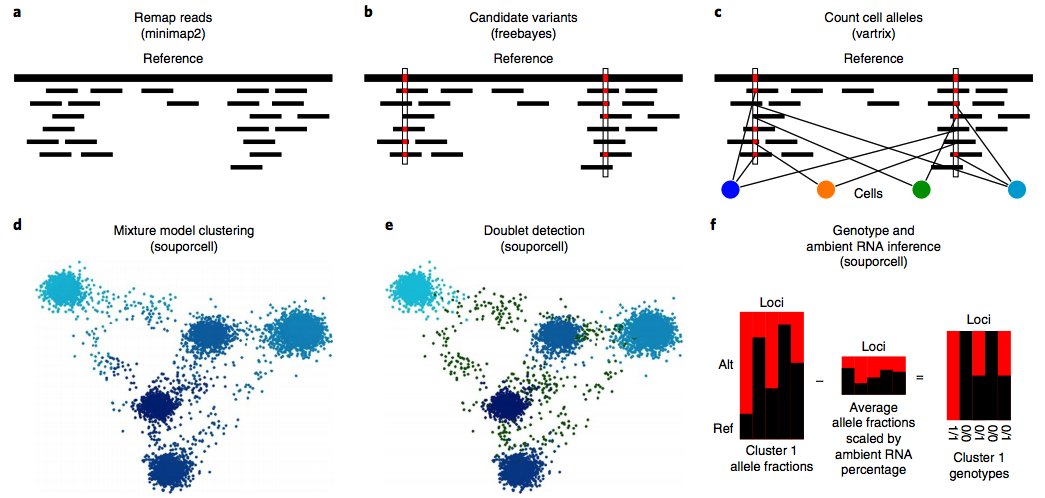
\includegraphics[width=\textwidth]{main.png} 
\end{centering}
\floatfoot{\small{\textbf{a)} First, the reads are remapped using minimap2, retaining the cell and UMI barcode for downstream use. b,c, Then candidate variants are called using freebayes \textbf{b} and count the allele support for each cell using vartrix \textbf{c}. \textbf{d)} Using the cell allele support counts, we cluster the cells with sparse mixture model clustering(Methods). \textbf{e,f)} Given the cluster allele counts, we categorize cells as doublets (\textbf{e}) or singletons and,
excluding doublets, the amount of ambient RNA is inferred along with the cluster genotypes(\textbf{f}; see example for one cluster). Alt, alternate allele;
ref, reference allele.}}

\end{figure}
\par{
I then demonstrate and benchmark souporcell against a dataset which was mixed in silico and thus we retain full knowledge of the ground truth of which barcodes came from which individual, which barcodes represent cross-genotype doublets, and how much ambient RNA was simulated(see figure \ref{figure:synthetic}). To show that this dataset is a realistic example, I then show the same results on an experimental mixture of cells from those same individuals(shown in figure \ref{figure:real}).
} 
\par{
I compare our method to demuxlet, the previous gold standard method that requires genotype information \textit{a priori}, as well as two new tools that, like souporcell, do not require prior genetic information\cite{vireo}\cite{scsplit} on the in silico mixture with various aspects of the data (doublet rate, ambient RNA amount, minority cluster size) swept and evaluate clustering, doublet detection, and ambient RNA detection across a wide range of data charactaristics. We sought to test souporcell on more challenging cases and chose that of highly related individuals by demultiplexing maternal-fetal placental and decidual experiments. We also test on mixtures of the malaria parasite, \textit{Plasmodium falciparum}, which is challenging due to the cells having much lower expression levels than the human cells previously tested.
} 
\par{
I show that souporcell not only outperforms the competing methods, but also surpasses the previous gold standard, demuxlet, on both cell assignment and doublet accuracy. Furthermore, souporcell explicitly models and estimates the amount of ambient RNA in the experiment, which is a major confounder of scRNAseq analysis with regard to both expression and genotype. Souporcell is freely available under the MIT open source license at \href{https://github.com/wheaton5/souporcell}{https://github.com/wheaton5/souporcell}.
}


\section{Methods} %Section - 1.1 
\subsection{Variant calling on scRNAseq data}
In order to use the genetic variants in the scRNAseq reads to assign cells to individuals, one must first call the variants accurately and assign which alleles were expressed by which cells. Little work has been done on identifying genetic variants in bulk RNAseq\cite{RNAvariant}\cite{somaticrna} let alone scRNAseq\cite{vartrix}\cite{cellsnp}. 



\subsubsection{Remapping}
\par{
Currently, the most popular software for the initial analysis of droplet based scRNAseq data to generate the mRNA expression matrix is cellranger\cite{10xsinglecell}. In the cellranger pipeline, the reads are first mapped to a reference genome. RNA mapping and DNA mapping software differ due to the intended downstream uses. With DNA mapping, accurate variant calling is one of the primary applications and thus much work has been put into providing accurate mapping quality scores and base level alignments making single nucleotide polymorphisms (SNPs) and short insertions and deletions (indels) easy to call accurately versus the reference genome used\cite{bwa}\cite{minimap2}\cite{bowtie}\cite{freebayes}\cite{gatk}. The mapping and alignment operations are relatively computationally costly if accurate variant calling is not one of the desired downstream uses. RNA mapping applications are usually primarily concerned with just counts of reads per gene and sometimes differential RNA splicing. Thus, the RNA community has developed software some of which are faster but do not provide base level alignments\cite{kallisto}\cite{salmon} and others that allow for gapped alignments caused by the introns being spliced out\cite{bowtie2}\cite{STAR}\cite{hisat}\cite{tophat}. But in optimizing for the downstream applications of transcript counting and differential splicing, genetic variant calling accuracy can suffer. In cellranger, the mapping component is done with the STAR aligner\cite{STAR} which, while sufficient for the purpose 
of counting gene expression, produces artifacts in the alignments that produce many false positive variants. 
} 
\par{
One such source of false positives is the 
soft clipping penalty which is not a parameter exposed to the user in the STAR software. It is often the case in WGS and even more so in RNAseq that the starts and ends of
reads can be less reliable than the rest of the read. In addition to this, base level alignments toward the ends of reads can be error prone because there is not a sufficient amount of sequence remaining for the ``correct'' alignment to be the optimal alignment according to the alignment score. For example, an alignment may prefer to take several single base mismatch penalties rather than a single true indel penalty. This tradeoff is more likely to happen towards the end of the read when there are fewer bases remaining to align (see figure \ref{fig:softclipping}b). Because of this, mappers built for variant calling such as BWA\cite{bwa} and minimap2\cite{minimap2} have 
a relatively small one-time penalty for soft clipping any number of bases from the end of an alignment\cite{variantartifacts}. The STAR alignment soft clipping penalty is such that, in 
comparison with other aligners, it can create many false positive variant calls produced entirely by bases at the ends of reads (see figure \ref{fig:softclipping}b). Another source of 
small variant errors caused by the STAR alignments is that the default indel penalty relative to the mismatch penalty is much higher than that of 
variant calling ready aligners. These penalties will, for example, prefer inducing 10 single base mismatches rather than a single 12 base indel. Further, it will make the same error for reads spanning the indel but not make the error for reads not spanning the indel causing those mismatches to potentially appear to be heterozygous genetic variants. 
}


\begin{figure}[htbp!]


\begin{centering}
\caption{Star alignments' indel and soft clipping problems}\label{fig:softclipping}

%\begin{subfigure}{0.75\textwidth}
\sidesubfloat[]{
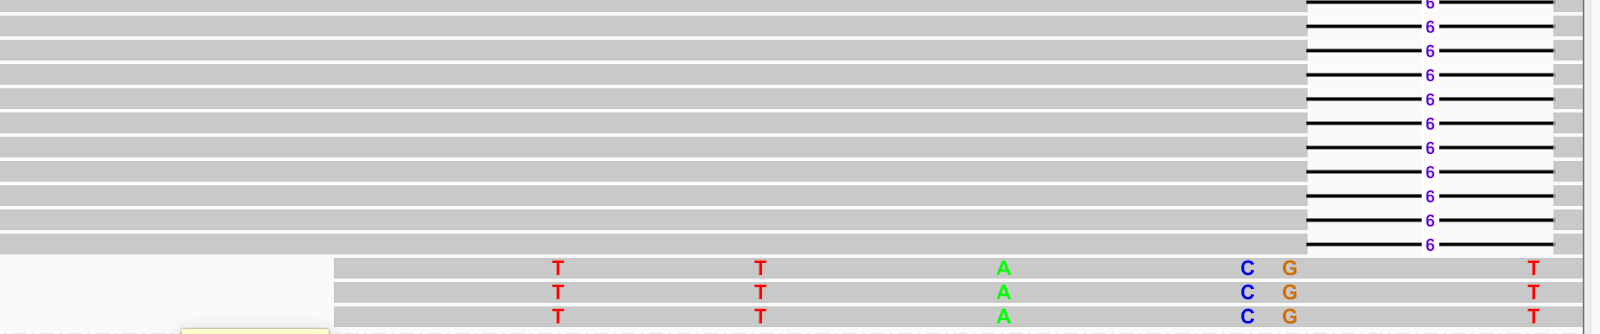
\includegraphics[width=0.75\textwidth, valign=t]{star_indel_issue.png} \label{fig:a}
}
%\end{subfigure}

%\begin{subfigure}[t]{0.75\textwidth}
\sidesubfloat[]{
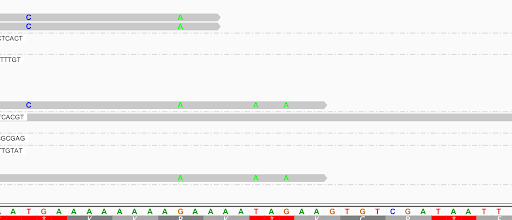
\includegraphics[width=0.75\textwidth, valign=t]{softclipping.png} \label{fig:b}
}
%\end{subfigure}
\end{centering}
\floatfoot{\small{\textbf{a)} Reads that span more bases find a six base indel, but ones that span fewer bases incur many erroneous single base mismatches without soft clipping. Minimap2 finds this indel in all of the shown reads and soft clips some others with even later start positions. \textbf{b)} In the second example, the reads have an adenosine homopolymer and partially match this section of the reference. Minimap2 softclips these reads. }}

\end{figure}
\par{
The indel penalty is exposed as a parameter to the user, but with the default parameters (and thus with the output of cellranger) these errors exist. 
And finally, the last source of errors these alignments induce are due to the leniency of spliced alignments which STAR has. With its default parameters including 
a max intron length of 200kb, STAR will often include erroneous and statistically spurious spliced alignments of reads that otherwise don't align well. This creates alignments 
which match for some statistically significant portion in one location and then are spliced to other loci often for as low as an eight base segment which should occur by 
random chance alone. Due to the nature of mapping qualities being assigned to the whole alignment and not each segment of the alignment, these sections are often denoted as 
having a high mapping quality when in fact the matches should occur by chance. If there is actually an alternative allele in one of these regions to which some reads have 
spurious matches, those reads, and thus those cells, appear to support the reference allele. These alignments provide one further technical 
issue, which is that they dramatically slow down the pileup and fetch commands in samtools\cite{samtools} which are necessary for variant calling. 
} 
\par{
For these reasons first the reads are remapped with either BWA, minimap2, or hisat2. I have found good results when remapping with minimap2 with a combination 
of long read splice parameters and short read parameters. Specifically, the parameters for which all analysis is done in this thesis are the following: 
minimap2 -ax splice -t 8 -G50k -k 21 -w 11 --sr -A2 -B8 -O12,32 -E2,1 -r200 -p.5 -N20 -f1000,5000 -n2 -m20 -s40 -g2000 -2K50m --secondary=no. Then, PCR duplicates are removed by identifying reads with the same unique molecular identifier (UMI) barcode, cell barcode, and have the same start and stop position.
}


\subsubsection{Variant Candidate Calling}
\par{
Once the reads are accurately mapped and aligned, one must then proceed to variant calling. I assessed two strategies for calling variants on scRNAseq and assigning alleles to cell barcodes. I first treated 
the sample as a population of cells and called variants with a population variant caller\cite{freebayes} \cite{gatk} \cite{samtools}. With this approach I assigned each cell barcode to its own read group in the input bam and the variant caller produces a population VCF with genotype calls for each cell for each locus.
I also assessed treating the sample as an unknown mixture of haplotypes, called variants on that unknown mixture, and then for each read (and thus its cell barcode) decide whether it supports the reference allele or alternative allele which can be done with the tool vartrix\cite{vartrix}. Our analysis suggests these two strategies perform very similarly. Because the latter strategy is much more computationally efficient, all further analysis is done with freebayes with parameters --pooled-continuous -iXu -C 2 -q 20 -n 3 -E 1 -m 30 --min-coverage 6 and vartrix with parameters  --umi --mapq 30 --scoring-method coverage which will return a sparse matrix market format indicating how many of the reference allele or alternative allele each cell barcode expressed for each variant locus.
}
\subsubsection{Cell allele assignment}
\par{
 Vartrix works by aligning each read to the reference sequence as well as the variant sequence to determine which one it supports. Doing this rather than simply inspecting the base level alignment improves reference bias and alignment end effects. For example, when assessing if a read supports an insertion of an A in a homopolymer of adenosines and the read does not extend past that homopolymer, the read will align without the insertion even if it came from the haplotype with the insertion. Aligning to both underlying sequences will produce the same alignment score and it is ambiguous which allele the read represents.
}
\subsubsection{Validation: Genome in a Bottle}
\par{
We validated our variant calling accuracy by obtaining from 10x Genomics an scRNAseq dataset run on cells from the Genome in a Bottle (GIAB) consortium individual NA12878 cell line for which there is high quality ground truth variant calls available\cite{giab}. As the scRNAseq data will only cover a subset of genes and because this dataset was relatively low coverage, I will primarily focus on false positive rate and not sensitivity. Much of this analysis was done by Yichen Wang as part of a rotation project in our lab. Initially we found a false positive rate of 35.6\%, dramatically higher than the 1-2\% you would have with reasonable coverage whole genome DNA sequencing.
}


\subsubsection{RNA editing}
\par{
We sought to determine the causes of the remaining false positives so identified the false positive SNPs called on the NA12878 scRNAseq data in high confidence regions as defined by the GiaB resource and found that most (80.8\%) of them are purine-to-purine or pyrimidine-to-pyrimidine transitions when we considered the reference and observations. A-to-G and T-to-C transitions happened in much higher frequency than the remaining, making up 59.5\% of
total false positive sites (see table \ref{table:rnaediting}). Calling variants from bulk RNA sequencing data also
displayed a similar pattern, but using whole exome sequencing data did not, linking the
excessive purine-to-purine and pyrimidine-to-pyrimidine transition specifically to RNA seq. We hypothesized that this could be due to RNA editing. The most common RNA editing event is the
deamination of adenosine to inosine on pre-mRNA\cite{atoi}. Inosine is then read as guanosine by
reverse transcriptase, resulting in a T-to-C event in the cDNA, which can explain A-to-G and T-to-C SNPs in variant calling. Visualization in the Integrative Genomics Viewer\cite{IGV} validated the
existence both reads with the false positive allele and reference allele in SNP loci. Moreover, we observed
that the reads that had the same UMI contained the same allele, but not the reads that had
the same cell barcode. This further supported the hypothesis of RNA editing, because the the reverse transcriptase reading inosine as guanine would be consistent for PCR duplicates of the cDNA, but
not necessary for all reads in one cell. And if these were due to sequencing errors, they would not be consistent across all PCR duplicates. To test the hypothesis of RNA editing, we found an RNA editing database (REDIportal\cite{rnaediting}: http://srv00.recas.ba.infn.it/atlas/) and removed the known A-to-I editing sites in our vcf files.
Filtering out RNA editing sites considerably reduced the amount of false positive variants (from
2884 to 1937) and kept most true positive variants (from 8093 to 8073), leading to a reduction
in false positive rate from 35.6\% to 24.0\%. We also discovered that remapping with hisat2
could further reduce false positive rate and improve sensitivity (9540 true positive loci ,1065
false positive loci, false positive rate 11.1\%). However, this work was done after the souporcell paper was published, so the results in this thesis are done with the minimap2 alignments as previously stated.
}

\begin{table}[htb]

\begin{centering}
\caption{RNA editing as a source of false positive variant calls}\label{table:rnaediting}
\sidesubfloat[]{
\begin{tabular}[htb]{|c|c|c|c|c|}\hline

\backslashbox{ref}{obs}&A&T&C&G \\\hline

A & 0 & 54 & 69 & 867 \\\hline
T & 55 & 0 & 849 & 80 \\\hline
C & 77 & 289 & 0 & 75 \\\hline
G & 326 & 68 & 70 & 0 \\\hline
\end{tabular}\label{fig:a}}
\hfil
\sidesubfloat[]{
\begin{tabular}[htb]{|c|c|c|c|c|}\hline

\backslashbox{ref}{obs}&A&T&C&G \\\hline

A & 0 & 54 & 69 & 395 \\\hline
T & 55 & 0 & 376 & 80 \\\hline
C & 77 & 289 & 0 & 75 \\\hline
G & 326 & 68 & 70 & 0 \\\hline
\end{tabular}\label{fig:b}}
\end{centering}

\floatfoot{\small{\textbf{a)} False positives are primarily purine to purine and pyrimidine to pyrimidine with a notable increase in A->G and T->C caused by the RNA editing adenosine to inosine. The inosine base is then read as a guanine by the reverse transcriptase. \textbf{b)} shows the false positive profile after filtering known RNA editing sites.}}



\end{table}



\subsection{Sparse mixture model clustering}
\par{
In order to introduce this method, I must first motivate it with a description of the data type and its particular difficulties with respect to clustering by genotypes. Each cell barcode has reads from its transcription profile sampled very sparsely. In table \ref{table:scdatatable} I show some basic statistics about two datasets --- one with a mixture of six strains of the malaria parasite \textit{Plasmodium falciparum} which is a unicellular haploid parasitic organism and the sample contains cells coming from all cell types found in the life cycle in the human blood stage. And the other data set is a mixture 
of five human individuals from the human induced pluripotent stem cell project. A filter is used requiring at least four cells supporting each allele otherwise the variant is unlikely to be of almost any use in discriminating between different genotypes in this mixture. 
As you can see, the number of cells expressing any given locus is far fewer than the total number of cells and the number of variants with a given number of cells expressing that variant drops off dramatically as cells expressing a given locus increases. It is also evident that while the human data contains more discriminating variants per cell, they are spread over many more total variants thus making the overlap between any two cells very low.
}

\begin{figure}[th!]
\caption{Single cell sparsity}
\label{figure:scdatafigure}
\begin{centering}
%\begin{subfigure}[b]{\textwidth}
\sidesubfloat[]{
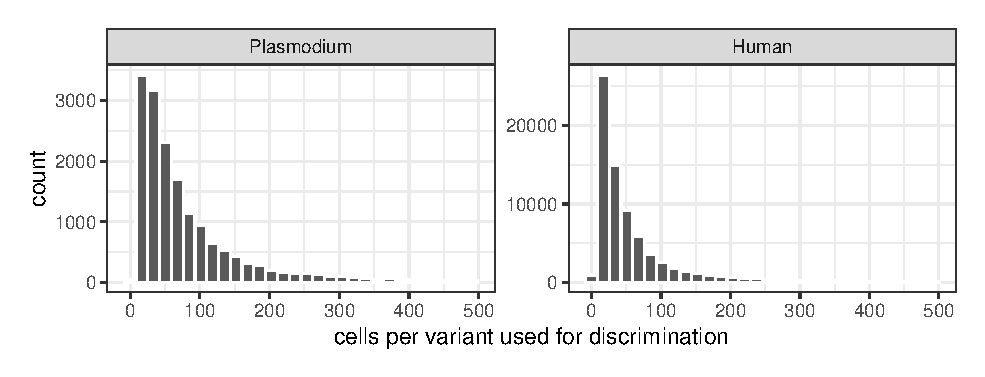
\includegraphics[width=\textwidth]{Cells_per_variant.eps} \label{fig:a}
}\\
%\end{subfigure}
%\begin{subfigure}[b]{\textwidth}
\sidesubfloat[]{
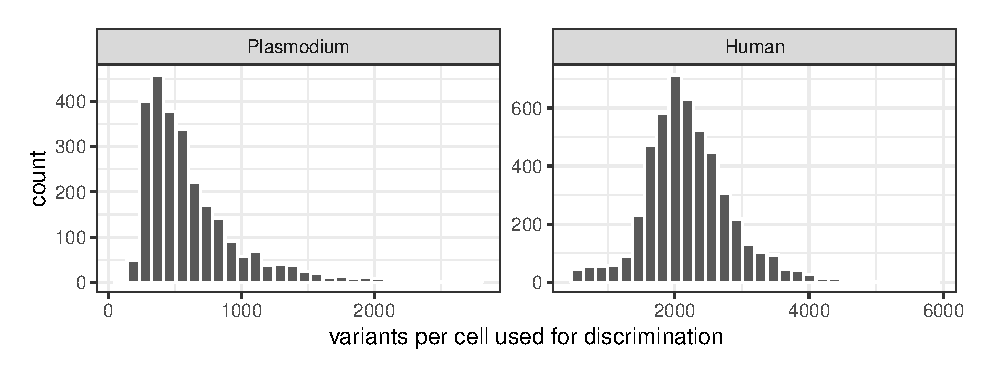
\includegraphics[width=\textwidth]{Variants_per_cell.eps}\label{fig:b}
}
%\end{subfigure}
\end{centering}
\floatfoot{\small{\textbf{a)} Shows the distribution of number of cells that have each variant and \textbf{b)} shows the distribution of the number of variants expressed by each cell. Both of these are subset to only consider variants that are used for discrimination. A variant is used for discrimination if it has at least four cells expressing the reference allele and four cells expressing the alternative allele.}}

\end{figure}

\begin{table}[h!]
\caption{Single cell data statistics}
\label{table:scdatatable}
\begin{center}
\begin{tabular}{ | l | l | l | } 
 \hline
  & malaria & human replicate 1 \\ 
  \hline
  number of cells & 2608 & 4925  \\
 \hline
  median UMI per cell & 995 & 25155  \\ 
 \hline
 total variants & 39487 & 194079 \\
 \hline
 median cells per variant & 24 & 18 \\
 \hline
 median variants per cell & 667 & 2642  \\ 
 \hline
 total discriminating variants & 16783 & 77878 \\
  \hline
 median discriminating variant per cell & 512 & 2147 \\
 \hline
 median cells per discriminating variants & 55 & 38 \\
 \hline
 median genes per cell & 571 & 4812 \\
 \hline
 
\end{tabular}
\end{center}
\end{table}

\par{
To describe the souporcell clustering algorithm, I will start by making some definitions. \\
} \\
\textbf{Definitions:}
\begin{itemize}
\item $K$: number of genotype clusters to be fixed at the outset. Lower case k will be used for indexing and referring to a specific cluster.
\item $C$: number of cells. Lower case c will be used for indexing and referring to a specific cell barcode. This barcode could have 0, 1, or more cells. It is important for some assumptions in this model that the majority of barcodes contain a single cell. 
\item $L$: number of variant loci. Lower case $l$ will be used to index and refer to a specific locus. Only biallelic variants are used. $L_c$ will be a list of loci with observed data in cell $c$.
\item $A$: Allele counts. $A_{l,c}$ is a vector of size 2 with the first number representing the number of reference alleles and the second representing the number of alt alleles seen at locus $l$ in cell $c$.
\item $\phi_{k,l}$: cluster center value representing allele fractions of cluster $k$ at locus $l$. This is a real number representing the fraction of ref alleles in this cluster at this locus. The expected values should be near 1.0 (homozygous reference), 0.5 (heterozygous), or 0.0 (homozygous alt) but will be skewed from these values by noise, doublets, and ambient RNA. 
\item $T$: temperature parameter for deterministic annealing process which is described later.

\end{itemize}

\noindent
\subsubsection{Model}

A maximum likelihood strategy is used by maximizing $\mathcal{L}(data)$ under a given model. 
\begin{equation}
\argmax_{\phi} \mathcal{L}(data, \phi)
\end{equation}

The likelihood of the data, treating cells independently and marginalizing each cell across the clusters it could belong to, is defined in equation \ref{equation:likelihood}. At each locus the alternate allele count is modeled by a binomial with $n$ as the reference + alternative allele counts for that cell at that locus and $\phi_{k,l}$ as the cluster center value representing the allele fraction for cluster $k$ at locus $l$.

Cluster model Likelihood function

\begin{equation}\label{equation:likelihood}
\mathcal{L}(A) = \prod_{c \in C} \sum_{k \in K} \frac{1}{K} \prod_{l \in L_c} {A_{l,c,0} + A_{l,c,1}  \choose A_{l,c,1}} \phi^{A_{l,c,1}}_{k,l} (1-\phi_{k,l})^{A_{l,c,0}}
\end{equation}
This model deals with sparsity naturally because if a cell has zero reference alleles and zero alternate alleles, a binomial with any probability, zero observations, and zero trials has a probability of one. Instead of uselessly multiplying many ones together, sites for which a cell has no alleles can be ignored.
One could then maximize this likelihood with random initialization of cluster centers $\phi \in (0,1)$ followed by expectation maximization (EM), but there are some problems one can run into.

\subsection{Deterministic Annealing} 
\par{
This method, as is the case with many clustering algorithms, may suffer from local optima in instances of poor initialization of the cluster centers $\phi$. This problem increases dramatically as the number of clusters increase. A standard solution to this problem is to have multiple restarts with random cluster center initializations, but as the number of clusters grows, the number of random restarts necessary to obtain the optimal clustering with high probability is unsustainable\cite{kmeansiterations}\cite{kmeansslow}. In addition to this, the sparse nature of the data increases the potential for local optima in the EM process. The two local optima clustering may produce is when one individual is split across multiple clusters and when multiple individuals are assigned to the same cluster. Some cells will express certain loci and other cells will express other loci. This means that given a random initialization of cluster centers, some cells from individual 1 may initially be more similar to one cluster center and other cells from the same individual may be more similar to a different cluster center because they happened to express different loci and the random initialization happened to fall a particular way. This may lead two cluster centers to be optimized for one individual. }

\par{Another approach to overcoming local optima in clustering is to initialize the cluster centers intelligently. The most simple initialization strategy is to initialize cluster centers to the values of individual data points (a particular cell in this case) as opposed to randomly in the space, but due to the sparse nature of the data, this would only assign a small minority of the dimensions, the rest of which would need to be random. Other smart cluster center initializations such as kmeans++ are also not particularly applicable to sparse datasets\cite{kmeanspp}. Not having access to these cluster center initialization strategies is limiting and makes it more likely that at initialization, multiple individuals' cells will match a single cluster.}
\par{ Without intelligent cluster center initialization as an option, I turned to methods which are better able to find their way out of local optima. Expectation maximization is known to be less susceptible to local optima as compared to kmeans clustering due to the logsumexp formula which is a smooth maximum (often called softmax) that falls out of marginalizing each data point across all clusters in log space\cite{KHM}. Another clustering algorithm---K harmonic means---uses a similar technique choosing the harmonic mean of the distances from a datapoint to all clusters rather than K means' distance to the closest cluster center (the min function) as a loss function to be optimized. The harmonic mean can be thought of as a smooth minimum function. Both of these strategies allow a datapoint to partially affect cluster centers that are not their current best cluster center. Over time, this can lead a cluster center that is not currently the best cluster for many data points to drift towards the ones that are closest to it. As it does so, it may reduce the impact those data points have on another cluster. The combination of these effects tends to improve both of the primary error modes of clustering---splitting a true cluster across two cluster centers and assigning data points from multiple true clusters to a single cluster center. These soft maximum and soft minimum functions can be thought of as a continuous spectrum of how soft, or smooth, they are---from min or max to uniform. The shape of these functions between these extremes also matter, but the degree of smoothness tends to matter more. A comparison of these functions can be seen in figure \ref{figure:softmax}. 
}


\begin{figure}[th!]
\caption{A comparison of smooth minimum and maximum functions}
\label{figure:softmax}
\begin{centering}
%\begin{subfigure}[b]{\textwidth}

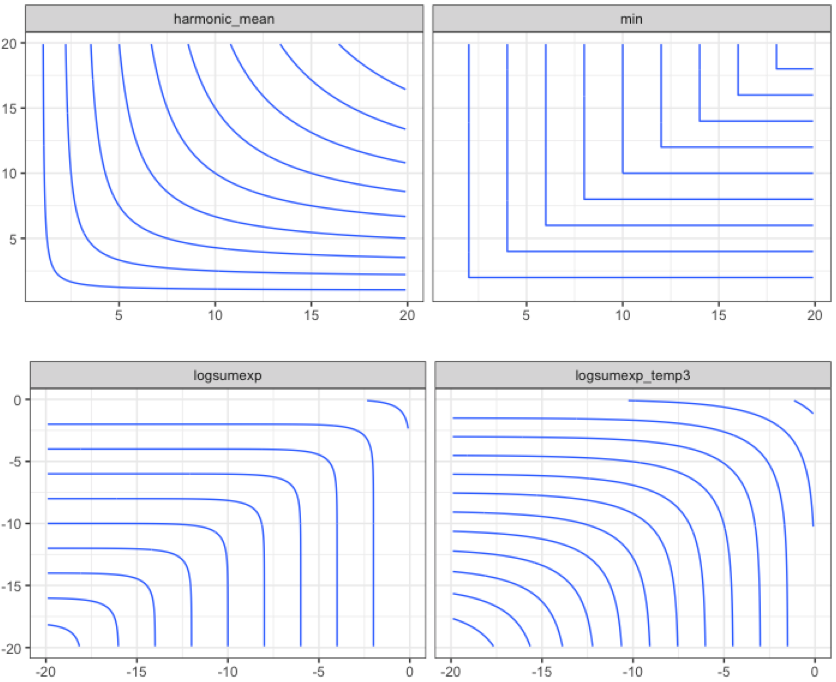
\includegraphics[width=0.75\textwidth]{softmax.png} 
\end{centering}
\floatfoot{\small{Harmonic mean is smoother than logsumexp, but applying an annealing temperature to logsumexp can make it arbitrarily smooth.}}
%\end{subfigure}
%\begin{subfigure}[b]{\textwidth}

%\end{subfigure}

\end{figure}


\par{
There is another method, deterministic annealing\footnote{Rather than knowing or finding this method, I rediscovered it. As my friend Peter Goldstein says, ``any wheel worth inventing is worth reinventing''. I initially used the binomial loss function and had poor results. I implemented a sum of squared differences loss function and had much better results. I moved on and attempted to publish the work. Reviewer 2 was asked why I didn't use the binomial loss function. I considered telling him that I tried it and the sum of squares loss function worked better. But this was unsatisfying. So I dug into why this was the case and the reason was that initially the likelihoods from the binomial loss preferred one cluster over another so much from the first step of random initialization, that they might never change to another cluster. This made me think of simulated annealing with the softening of the likelihood search space. I formulated the equivalent mathematical adaptation that that stochastic process took to this deterministic process which ended up being the same as this method published 22 years earlier. Satisfying, but perhaps I should have just done a more thorough literature search at the outset. }, which allows the degree of how smooth the function is across the optimization process\cite{annealing}\cite{annealing2} (see figure \ref{figure:softmax}). Deterministic annealing, similar to the older and more widely known simulated annealing\cite{simannealing}, takes its namesake from a process in metallurgy in which a metal object is heated to a high temperature and then cooled slowly in a controlled fashion that improves the molecular crystal structures and alters certain properties of the resulting product. They take their mathematical inspiration from statistical mechanics by treating the negative log likelihood as the energy of the system and in an attempt to find the minimum free energy, apply a temperature which begins high and is slowly reduced over time. The temperature dictates the degree of trade-off between exploration of a search space and exploitation of local gradients in the likelihood landscape. }

\par{Because the problem lends itself to a simple statistical model and deterministic annealing allows us to vary this tradeoff throughout the optimization process, I chose the deterministic annealing variant of expectation maximization for our clustering algorithm. The annealing process requires us to choose a meta-heuristic which is the temperature schedule. In deterministic annealing, the starting temperature is more important than in simulated annealing. With simulated annealing, a high temperature simply means a uniform search over the space regardless of the likelihood landscape. In deterministic annealing applied to clustering, if the temperature starts too high, it makes the data point's posteriors for each cluster uniform. After a few iterations of expectation maximization, the cluster centers may all be nearly identical making the gradients going forward vanishingly small leading to a symmetry breaking local optima. How smooth the soft max function needs to be is a function of the magnitude of the log-likelihoods of each data point, which, in this application, is largely dictated by how many alleles each cell expresses. Through empirical experimentation, I chose to initialize our temperature to one tenth the average number of alleles expressed by each cell. At each temperature step expecation maximization is run until the change in total log likelihood between steps is minimal (<0.1) which is used as the criteria of convergence. At each new temperature step, the temperature is halved until it is less than one at which point a final step is run at a temperature of one which reduces to the original likelihood function in equation \ref{equation:likelihood}. Cluster centers are randomly initialized and the optimization is run 50 times by default and the solution with the maximum total likelihood is chosen as the best solution. At each temperature step, a temperature modified posterior for each cell belonging to each cluster is defined as follows.
}

\begin{equation}
p_T(c \in k) =  \frac{e^{\frac{\log(\mathcal{L}(A_{c,k}))}{T}}}{\sum_{i \in K} e^{\frac{\log(\mathcal{L}(A_{c,i}))}{T}}}
\end{equation}
Which gives our maximization step according to the following equation.
\begin{equation}
\phi_{k,l}' = \frac{\sum_{c \in C} A_{l,c,1} p_T(c \in k)}{\sum_{c \in C}(A_{l,c,1} + A_{l,c,0})p_T(c \in k)}
\end{equation}

\par{
In figure \ref{figure:annealing} you can see that deterministic annealing is better able to find the global optimum likelihood than expectation maximization and that even when it seems to be stuck in a local optimum, as is seen in the log likelihood plateaus in the graph, it is much more likely to find its way out. This becomes much more extreme as the number of individuals, or clusters, there are. And interestingly it also becomes more extreme as the amount of data per cell increases. This may be counter intuitive as you would think the amount of data per cell would make it easier to find the optimal clustering. But instead, the additional data makes the posterior probability for each cell to a cluster be closer and closer to zero or one even at a given random initialization of cluster centers. As the amount of data increases, the log likelihoods are of higher magnitude and the smoothness of the logsumexp function at higher magnitudes is less. The result of this is that it is very common for a given cluster center to be highly preferred over other clusters potentially for multiple individuals' cells and their effect on other clusters to be vanishingly small. This is why it is important both to use deterministic annealing as well as to use the amount of data per cell as a guide for the starting temperature.
}


\begin{figure}[th!]
\caption{EM vs Deterministic Annealing on four and eight individuals}
\label{figure:annealing}
\begin{centering}
%\begin{subfigure}[b]{\textwidth}

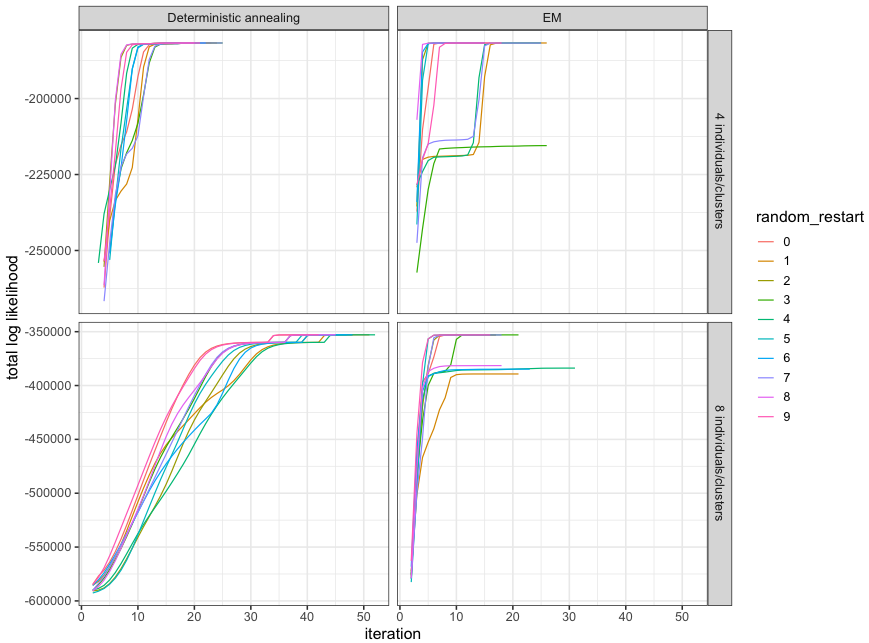
\includegraphics[width=0.75\textwidth]{annealing.png} 
\end{centering}
\floatfoot{\small{Deterministic annealing finds the optimal clustering (and thus highest likelihood) in all cases whereas EM fails in one random restart with four individuals. With eight individuals, EM fails in several random restarts while Deterministic annealing still finds the optimal clustering every time. This difference becomes much more dramatic with more individuals / clusters.}}
%\end{subfigure}
%\begin{subfigure}[b]{\textwidth}

%\end{subfigure}

\end{figure}


\subsection{Combinatorial experimental design for individual to cluster matching}
\par{
There has been some concern in the community that it will be difficult to know which cluster corresponds to which individual after deconvolution with multiplexed scRNAseq experiments when genotypes are not known a priori. To address this, I propose an experimental design involving $m$ overlapping mixtures for $2m-1$ multiplexed individuals outlined in table \ref{table:multiplex}. Each individual is assigned a binary number $1..2m$, where each bit corresponds to the inclusion (1) or exclusion (0) from each of the mixtures. This gives each individual a unique signature of inclusion/exclusion across the mixtures. Although each sample is in a different number of mixtures, the number of cells per experiment can be adjusted according to the number of mixtures that contain that sample. Souporcell provides a tool to match clusters from two experiments with shared samples.
}



\begin{table}


\caption{Experimental design for matching individuals to clusters}\label{table:multiplex}
\sidesubfloat[]{
\begin{tabular}[htb]{| l | c | c | c |}
%a & & & \\
\hline
Mixture & 1 & 2 & 3 \\
\hline
\hline
Individual a & 0 & 0 & 1 \\ 
\hline
Individual b & 0 & 1 & 0 \\  
\hline
Individual c & 0 & 1 & 1 \\  
\hline 
Individual d & 1 & 0 & 0 \\  
\hline 
Individual e & 1 & 0 & 1 \\  
\hline 
Individual f & 1 & 1 & 0 \\  
\hline 
Individual g & 1 & 1 & 1 \\  
\hline 
\end{tabular}\label{tab:a}}
\hfil
\sidesubfloat[]{
\begin{tabular}[htb]{| l | c | c | c | c |}
\hline
Mixture 1 & d & e & f & g \\
\hline
Mixture 2 & b & c & f & g \\
\hline 
Mixture 3 & a & c & e & g \\
\hline
\end{tabular}\label{tab:b}}
\floatfoot{\small{This table outlines an experimental design of seven individuals with three overlapping mixtures to allow for clusters to be assigned to individuals. \textbf{a)} Shows the mapping of individuals to binary numbers where each digit of the binary number represents inclusion/exclusion from a mixture. \textbf{b)} shows the resulting mixtures.}}

\end{table}




\subsection{Doublet cell barcode detection}
\par{
One of the major aims of this work is to detect the barcodes which contain multiple cells with different genotypes. 
I do not, however, attempt to detect barcodes which contain multiple cells with the same genotype. I make the assumption that 
the generation of doublet cell barcodes is a random poisson process and that the rate of this poisson process is low enough that 
the chance of droplets with more than two cells are exceedingly unlikely. This is true for the standard experimental design, but is not in the case of super loading cells into the system. As discussed in chapter 1, I advise against this for several reasons. I view this problem 
as an urn problem in which each cluster is an urn containing alleles expressed by all of the cells assigned to that cluster. Then each cell is inspected to determine if its alleles were more likely to be drawn from the single best cluster or the allele counts of
the combination of the top two clusters for this cell. \\
}  





\textbf{Definitions:}
\begin{itemize}
\item[$A_{k,l}$] Allele counts at locus l for all cells in cluster k according to the maximum probability cluster assignment from our clustering. This is a vector of size two with the ref and alt allele counts.
\end{itemize}

Allele counts of each cell at each locus are treated random variables drawn from a beta-binomial distribution from either a single cluster or a pair of clusters. The beta-binomial is used to model our uncertainty in the binomial parameter p. For a single cluster the parameters are alpha = 1+alt counts and beta = 1+ref counts. 
For the singleton case, the likelihood of the data is as follows.
\begin{equation}
\mathcal{L}(c \in K_i) = \prod_{l \in L_c} {A_{l,c,0} + A_{l,c,1}  \choose A_{l,c,1}} \frac{\beta(A_{l,c,0} + 1 + A_{i,l,0}, A_{l,c,1} + 1 + A_{i,l,1})}{\beta(1+A_{i,l,0} + A_{i,l,1})}
\end{equation}


Where $\beta$ is the beta function and cluster $i$ is the best fitting cluster for cell $c$. \\
The expected allele fractions of a doublet coming from cluster $i$, and cluster $j$ is the average of the allele fractions of the two clusters. To obtain the pseudocounts needed to parameterize the beta-binomial, the counts of alleles from the cluster with the fewer alleles at this locus are used. That is, 
\begin{equation}
alpha_{l,i,j} = 1 + \frac{\frac{A_{i,l,0}}{A_{i,l,0}+A_{i,l,1}} + \frac{A_{j,l,0}}{A_{j,l,0}+A_{j,l,1}}}{2}min(A_{i,l,0}+A_{i,l,1}, A_{j,l,0}+A_{j,l,1})
\end{equation}

\begin{equation}
beta_{l,i,j} = 1 + \frac{\frac{A_{i,l,1}}{A_{i,l,0}+A_{i,l,1}} + \frac{A_{j,l,1}}{A_{j,l,0}+A_{j,l,1}}}{2}min(A_{i,l,0}+A_{i,l,1}, A_{j,l,0}+A_{j,l,1})
\end{equation}
The doublet likelihood given those conservative parameters becomes
\begin{equation}
\mathcal{L}(c \in K_i \cup K_j) = \prod_{l \in L_c}  {A_{l,c,0} + A_{l,c,1}  \choose A_{l,c,1}}\frac{\beta(A_{l,c,0} + alpha_{l,i,j}, A_{l,c,1} + beta_{l,i,j})}{\beta(alpha_{l,i,j} + beta_{l,i,j})}
\end{equation}
The posterior for each cell being a doublet is then given by
\begin{equation}
p(doublet_c | c) = \frac{p(c \in K_i \cup K_j)p(doublet)}{p(c \in K_i \cup K_j)p(doublet) + p(c \in K_i)(1-p(doublet))}
\end{equation}
Where cluster $i$ is the best fitting cluster for cell $c$ and cluster $j$ is the second best fitting cluster for cell $c$. The prior can be set by the user but have used an uninformed prior of 0.5 for all of our analysis. 
\par{The above process is run iteratively removing doublets found until no new doublets are found.} 





\subsection{Ambient RNA detection and Cluster genotype coinference}
\par{One major goal of clustering scRNAseq by genotypes is calling the genotypes for each individual/cluster.
But as previously discussed, there can be lysed cells in solution prior to cell partitioning which contribute a background noise to both genotypes and transcriptional profiles. 
This ambient RNA gives a fuzzy picture of the transcriptional profile and makes cluster genotypes which are in truth homozygous appear heterozygous. 
Luckily with genotype mixtures, the prior knowledge of ploidy of the organisms can be used along with our genotype cluster assignments to 
make a co-inference of both the genotypes and level of ambient RNA in the experiment.}

\subsubsection{Mixture model of ambient RNA and cell RNA}
\textbf{Definitions:}
\begin{itemize}
\item $\rho$: probability any given allele is arising from ambient RNA as opposed to from the cell associated with that barcode. This will be learned.
\item $P$: ploidy. Currently, only ploidy of one or two is supported. 
\item $A_l$: total allele expression at locus l. This is again a vector of length 2 denoting the reference and alternative allele counts.
\item $g$: used to denote the number of copies of the reference allele. The expected reference allele rate without ambient RNA is $g$ and $g$ is an integer value $[0..P]$. Note that for biallelic variants and ploidy 1 or 2, $g$ is sufficient to uniquely determine the genotype. 
\item $p(true)$: prior for variant being a true variant vs a false positive. The default is 0.9 which was the value used for all analyses.
\end{itemize}


Once again, a maximum likelihood approach is taken.
\begin{equation}
\argmax_{\rho} \mathcal{L}(data, \phi)
\end{equation}

\par{
Here, the proportion of ambient RNA in the system, $\rho$, is the only free parameter and is optimized using maximum likelihood. The model treats each locus in each cluster as coming from one of three genotypes for diploid (0/0, 0/1, 1/1, here denoted by $g$ = 0, 1, or 2) and two genotypes from haploid (0, 1). Each cluster is treated as independent and each locus as independent, before marginalizing across the possible genotypes. The model also considers the possibility of the variant being a false positive. In this case, the variant will not segregate into distinct allele frequencies between different clusters and it will most likely not attain a value close to the standard allele frequencies expected from the diploid or haploid genotypes. Thus, the allele counts in each cluster are modeled as having come from a mixture of ambient RNA (an average allele fraction in the experiment) and from the cells in that cluster. The observed allele fractions are assumed to have been drawn from a binomial distribution with a probability that was skewed away from $p = g/P$ by the level of ambient RNA $\rho$. Thus, the probability of the binomial from which the allele counts are drawn for true positive variants is the following.
}



\begin{equation}
p_{tp} = (1-\rho)\frac{g}{P} + \rho \frac{A_{l,0}}{A_{l,0}+A_{l,1}}
\end{equation}
For a false positive the parameter is
\begin{equation}
p_{fp} = \frac{A_{l,0}}{A_{l,0} + A_{l,1}}
\end{equation}

Thus, the full model is
%\begin{equation}
%\begin{multline}
%\begin{split}
%p(data | \rho)  &= \prod_{l \in L} \bigg[p(true) \prod_{k \in K} \sum^P_{g=0} \frac{1}{P}  {A_{l,c,0} + A_{l,c,1}  \choose A_{l,c,1}} p_{tp}^{A_{k,l,0}} (1-p_{tp})^A_{k,l,1}  \\ &+ (1-p(true)) \prod_{k \in K} {A_{l,c,0} + A_{l,c,1}  \choose A_{l,c,1}} p_{fp}^{A_{k,l,0}} (1-p_{fp})^A_{k,l,1} \bigg]
%\end{multline}
%\end{split}
%\end{equation}


\begin{equation}
\begin{split}
p(data | \rho) = \prod_{l \in L} \bigg[ & p(true) \prod_{k \in K} \sum_{g = 0}^P \frac{1}{P} \binom{A_{k,l,0} + A_{k,l,1}}{A_{k,l,0}} p_{tp}^{A_{k,l,0}} (1-p_{tp})^{A_{k,l,1}} \\
 & + (1-p(true))\prod_{k \in K}\binom{A_{k,l,0} + A_{k,l,1}}{A_{k,l,0}}p_{fp}^{A_{k,l,0}} (1-p_{fp})^{A_{k,l,1}}  \bigg]
\end{split}
\end{equation}

\subsubsection{Inference}
We solve for $\rho$ with gradient descent using the statistical modeling domain specific language STAN. Next, the posterior of the variant being a true variant is calculated for each of the three (or two in the haploid case) genotypes versus it being a false positive. The prior on variants being true positives can be set by the user, but defaults to 0.9 which is the value used in our analyses.




%********************************** %Second Section  *************************************
\section{Results}



\subsection{Benchmarking: Synthetic human cell mixture}

Currently, there are no good generative models available for batch effects, allele-specific expression, ambient RNA, and doublets in scRNAseq that can be used to generate in silico data for testing methods that cluster by genotype. To generate realistic data with known ground truth we sequenced five lines of induced pluripotent stem cells (iPSCs) from the Human iPSC initiative\cite{hipsci} with the 10x Chromium single cell system, both individually and in a mixture of all five lines (with three replicates of the mixture). Each mixture contained 5-7,000 cells and ~25,000 UMIs per cell. We first synthetically mixed 20\% of the cells from the 5 individual samples while retaining their sample of origin. To make the synthetic mixture as close to real data as possible, I also simulated 6\% doublets by switching all of the reads' barcodes from one cell to that of another cell and 5\% ambient RNA by randomly switching cell barcodes for 5\% of the reads. A low dimensional representation of the expression matrix reveals relatively little variation, as expected, since there is only one cell type present (\ref{figure:synthetic}a). Indeed, the most significant driver of expression appears to be the donor of origin, but the donor cells overlap in expression patterns and it is not possible to assign a donor to each cell based solely on expression patterns.



\begin{figure}[th!]
\caption{Synthetic human mixture}
\label{figure:synthetic}
\begin{centering}

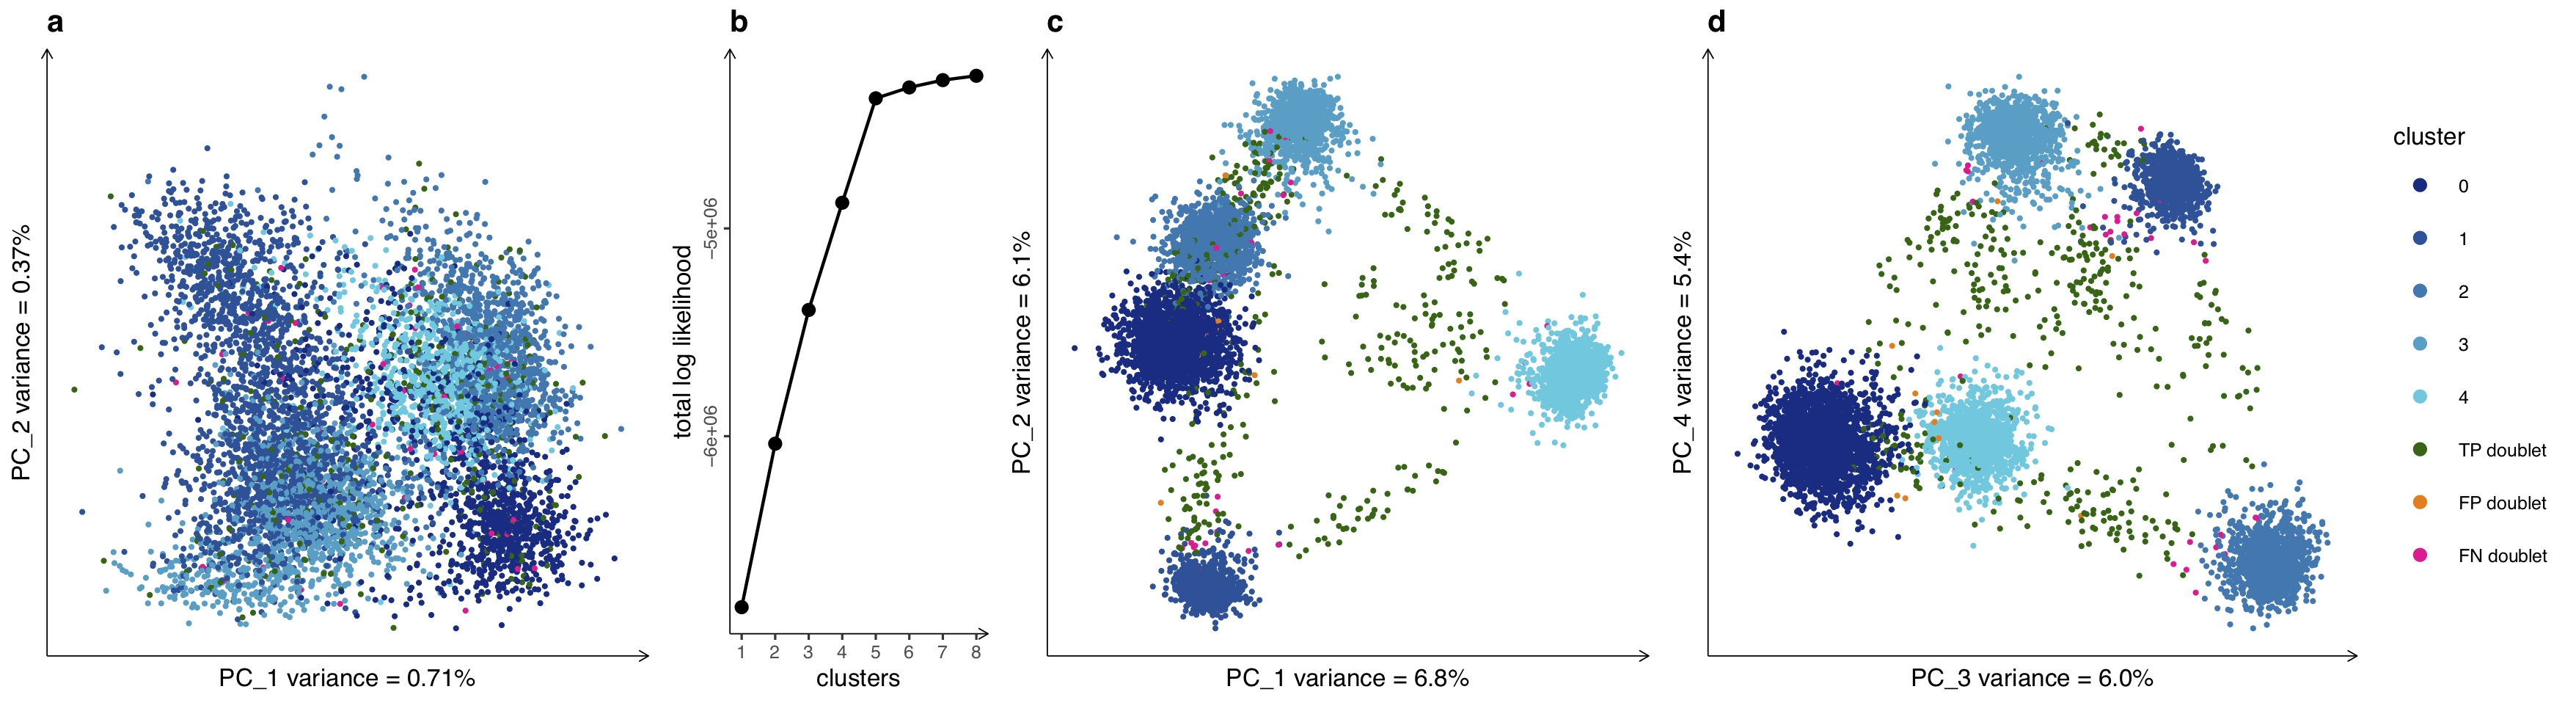
\includegraphics[width=\textwidth]{simulated.jpg} 
\end{centering}
\floatfoot{\textbf{a)} Expression PCA of a synthetic mixture cells from five HipSci cells lines (n=7073 cells) with 5\% ambient RNA and 6\% doublets colored by known genotypes. Because these samples only contain one cell type, the largest remaining source of variation in the expression profile comes from the genotype, although the signal is not sufficient for accurate genotype clustering. \textbf{b)} Elbow plot of the number of clusters versus the total log likelihood showing a clear preference for the correct number of clusters (k=5). \textbf{c} and \textbf{d)} PCA of the normalized cell-by-cluster log likelihood matrix from souporcell (n=7073 cells). As this is a synthetic mixture in which the ground truth is known, the genotype clusters are colored and errors are highlighted in orange (false positive doublets) and pink (false negative doublets).}


\end{figure}





\subsection{Benchmarking: Real human cell mixture}

Next I compare to a true mixture of human cells in which the ground truth is not known. The results (shown in \ref{figure:real} are strikingly similar to those in \ref{figure:synthetic} which suggest that our synthetic mixture is realistic. 

\begin{figure}[th!]
\caption{Experimental human mixture}
\label{figure:real}
\begin{centering}
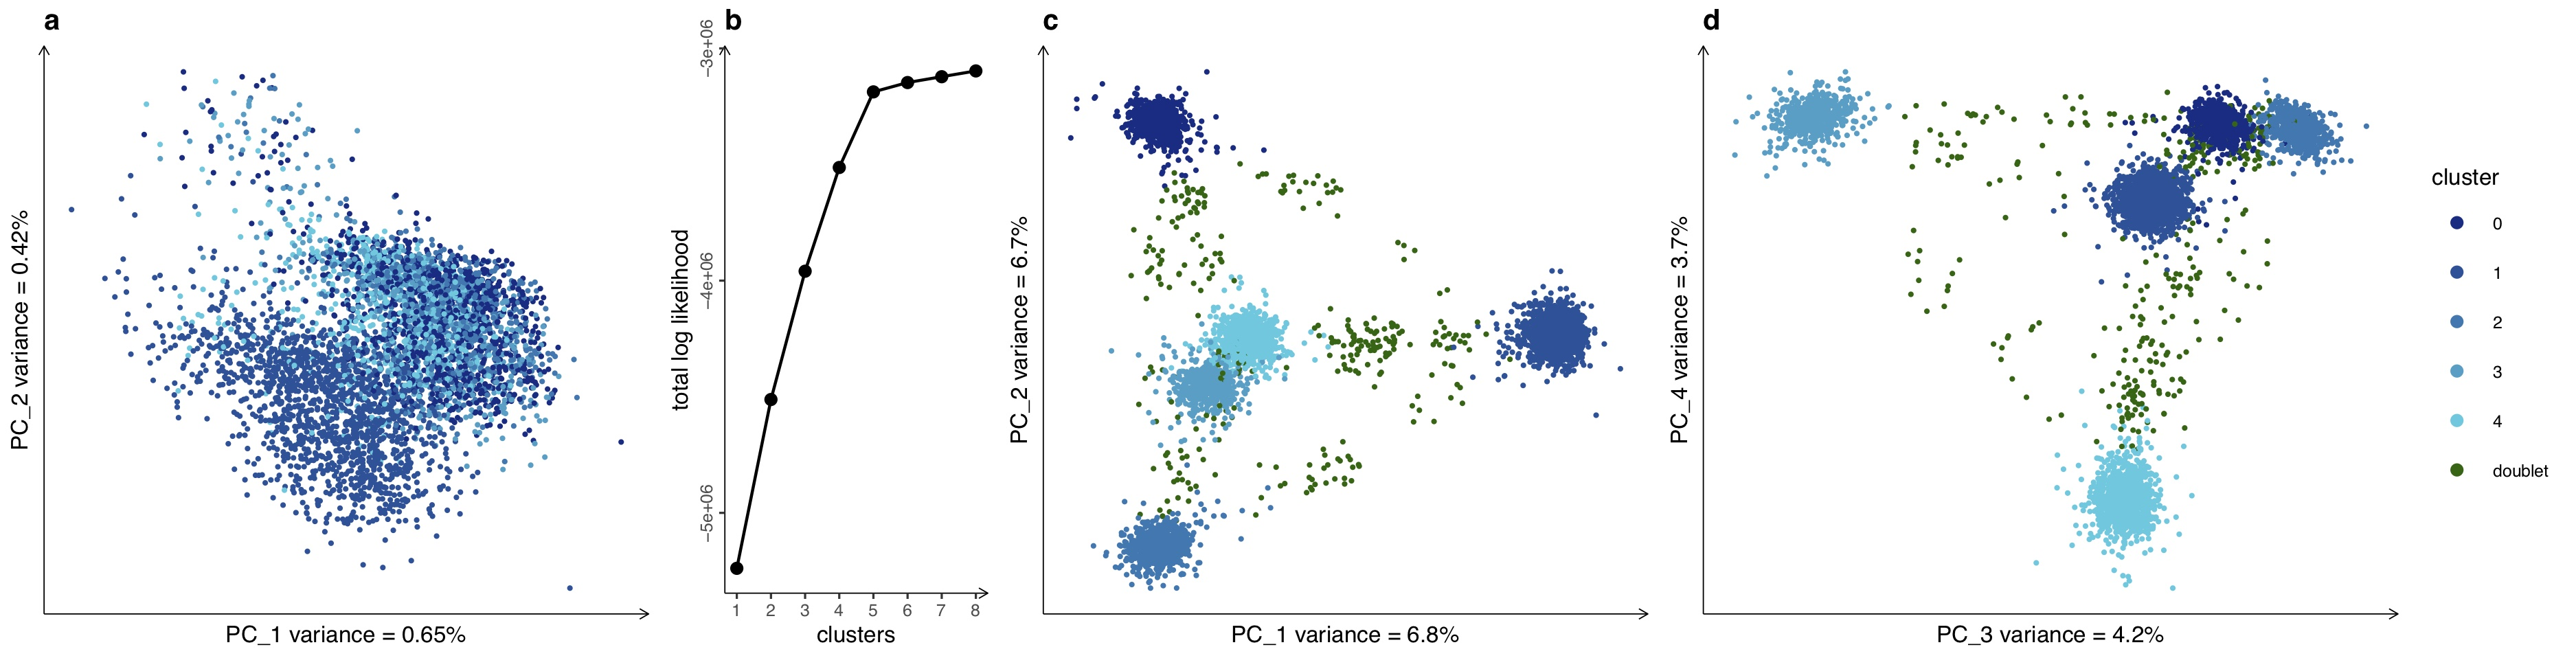
\includegraphics[width=\textwidth]{realmix.jpg} 
\end{centering}
\floatfoot{\small{\textbf{a)} Expression PCA of a single replicate (see Fig. S1 for reps) of the experimental mixtures (n=4925 cells) colored by genotype clusters from souporcell. \textbf{b)} Elbow plot of the total log likelihood versus different numbers of clusters showing a clear preference for the correct number of clusters. \textbf{c} and \textbf{d)} PCA showing the first four PCs of the normalized cell-by-cluster log likelihood matrix colored by cluster (n=4925 cells).}}
\end{figure}


%\begin{figure}[th!]
%\caption{Experimental human mixture replicates}
%\label{figure:humanreplicates}
%\begin{centering}

%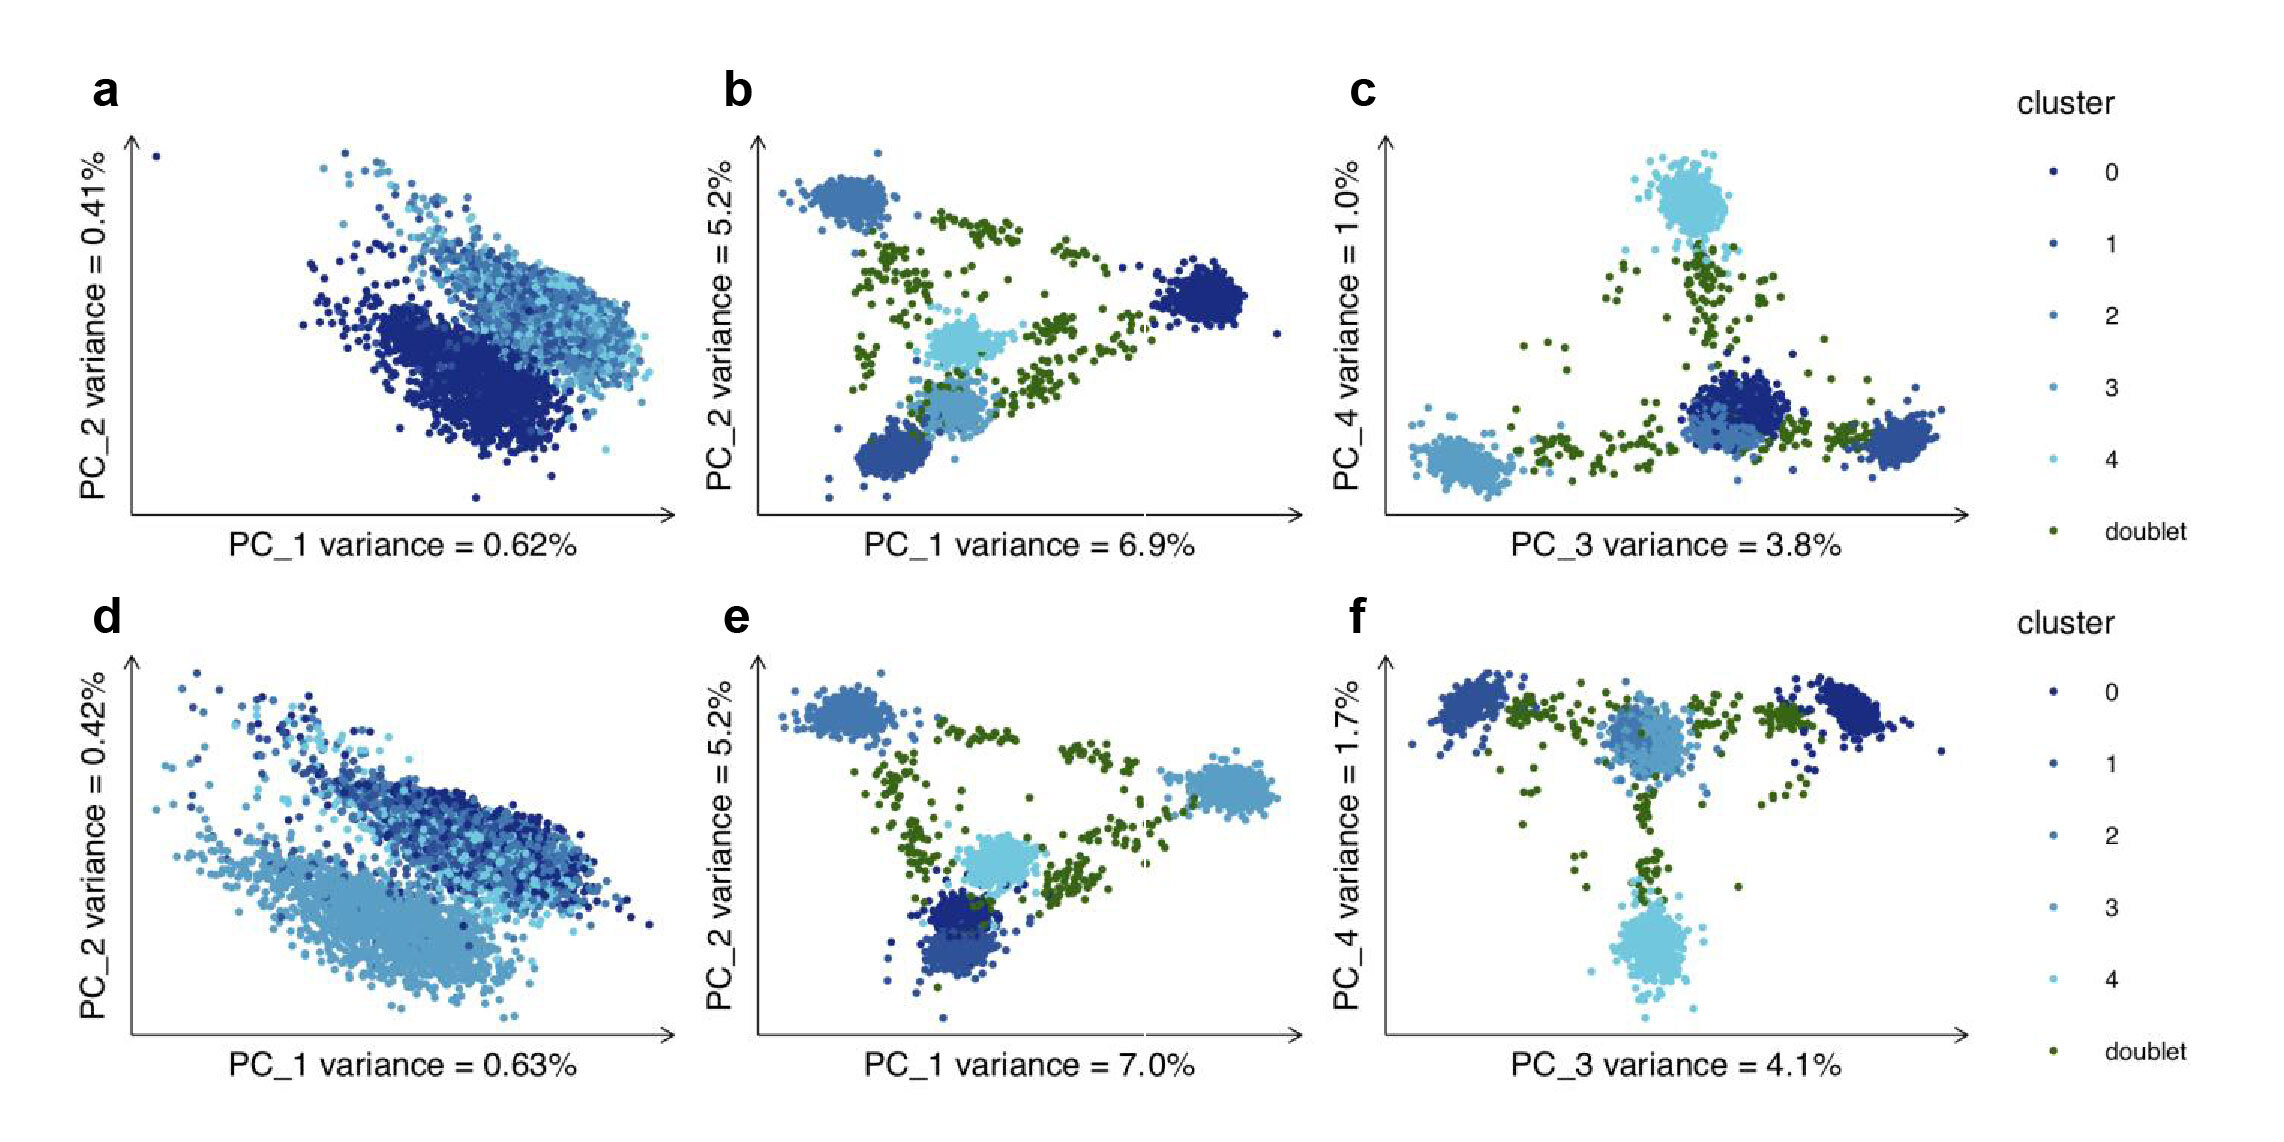
\includegraphics[width=\textwidth]{human_replicates.jpg} 
%\par{\textbf{a)} Expression PCA of a single replicate (see Fig. S1 for reps) of the experimental mixtures (n=4925 cells) colored by genotype clusters from souporcell. \textbf{b)} Elbow plot of the total log likelihood versus different numbers of clusters showing a clear preference for the correct number of clusters. \textbf{c} and \textbf{d)} PCA showing the first four PCs of the normalized cell-by-cluster log likelihood matrix colored by cluster (n=4925 cells).}
%\end{centering}
%\end{figure}


\subsection{Benchmarking: demuxlet paper dataset}

\par{
In order to demonstrate souporcell on an external and widely used benchmark dataset, I downloaded the
three overlapping mixtures from the demuxlet paper\cite{demuxlet}
. Sample A contains a mixture of four donors'
PBMCs, Sample B contains a mixture of four different donors? PBMCs, and Sample C contains a mixture
of all 8 donors' PBMCs. I synthetically combined this data into a single dataset and clustered with
souporcell. Figure \ref{figure:demuxlet}a shows that the resulting clusters either contain cells from Sample A or Sample B,
but not both as is expected from this experimental setup. I also show that the first cluster of the doublet
assignments are also largely consistent with this experimental design (figure \ref{figure:demuxlet}b). 
}

\begin{figure}[htbp!]
\caption{Demuxlet data}
\label{figure:demuxlet}
\begin{centering}
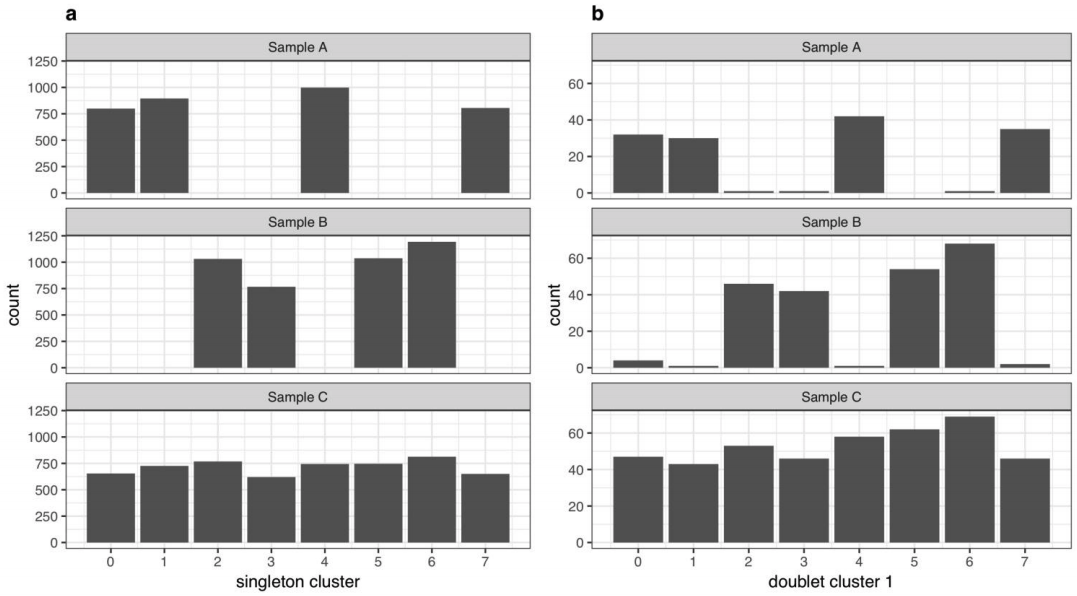
\includegraphics[width=\textwidth]{demuxletdata.png} 
\end{centering}
\floatfoot{\small{\textbf{a)} souporcell cluster assignments of singletons for combined dataset showing that Sample A and Sample B are non-overlapping and
Sample C contains all 8 samples. \textbf{b)} shows the first cluster of the doublet assignment for doublets showing largely non-overlapping
assignments between Samples A and B.}}

\end{figure}

\subsubsection{Deconvolution of overlapping mixtures}

\par{
To enable identification of which cluster is which individual using the overlapping mixture experimental
design outlined in Table 1, I provide a tool shared\_samples.py which takes as input two souporcell
output directories and the number of samples which are shared. It compares the sum of squared
differences of the allele fraction of confident (>95\% confident genotype call in all clusters) shared variant
calls between clusters in the two experiments and outputs the best matches for the number of shared
samples. I tested this using multiple synthetic mixtures of 5 HipSci
cell lines with 6\% doublets and 5\% ambient RNA and gave both as input to the shared\_samples.py tool
and it correctly assigned the clusters in one run to the clusters in the second experiment which
corresponded to the same samples. I also ran souporcell on the three demuxlet datasets separately and
ran the shared\_samples.py tool on Sample A vs Sample C and Sample B vs Sample C and it confidently
identified the non-overlapping clusters in Sample C which correspond to A and B. 
}



\subsubsection{Validation and comparison to other methods}

\par{
I compared souporcell to vireo and scSplit, two other tools that do not require prior genetic information. First, I ran variant calling and cell allele counting as recommended for each tool. Using souporcell, I clustered cells by their genotypes, and evaluated the correct number of clusters through an elbow plot comparing the total log probability versus a varying number of clusters (\ref{figure:synthetic}b). The clustering output can be viewed as a matrix with cells as rows and clusters as columns with the values being the log likelihood of that cell versus the corresponding cluster. To visualize the five clusters identified by genotype I carried out a PCA of the normalized log likelihood matrix, which reveals a clear separation of the clusters, with interspersed doublets (\ref{figure:synthetic}c and d).  For these data souporcell assigned 6612/6622 singletons and 415/451 doublets correctly; four singletons were falsely labeled as a doublet, 35 doublets were misidentified as singletons, and one doublet and four singletons were unassigned. I carried out the same analysis for the three replicates of the  experiment mixtures and show results for one (\ref{figure:real}). The expression PCA (Fig. 2e) and normalized cell-cluster loss PCA (\ref{figure:real}c,d) of the experimental mixture were similar to the synthetic mixture indicating that the synthetic mixtures were an accurate approximation of real mixtures. To compare doublet detection between methods, I calculated a receiver-operator characteristic (ROC) curve of the doublet calls (\ref{figure:compare}i) on a synthetic mixture with 6\% doublets and 10\% ambient RNA that showed the area under the curve values of 0.98 and 0.91 for souporcell and vireo, respectively. I also show point estimates for the doublet threshold chosen. Demuxlet's posterior doublet probability output did not have enough significant digits and is 1.0 until it starts varying with 27\% false positives. The default doublet probability threshold for demuxlet gives nearly 40\% false positive doublets.
} 

\par{
Each of the five human iPSC lines has existing WGS data generated as part of the HipSci Project\cite{hipsci2}. Therefore, for the experimentally mixed replicates, I compared each tool's clustering to sample assignments obtained from demuxlet using genotypes available from the WGS. Demuxlet significantly overestimates doublets versus expectations based on the number of cells loaded\cite{10xsinglecell} especially as ambient RNA increases (\ref{figure:compare}b). Because I could not trust the doublet calls of demuxlet, I allowed scSplit, vireo, and souporcell to exclude their called doublets and then compared the remaining cells to demuxlet's best single genotype assignment. The Adjusted Rand Index (ARI) of the remaining cell assignments versus demuxlet were 1.0 (fully concordant) for souporcell and vireo across the three replicates and an average of 0.97 for scSplit.
} 

\par{
To evaluate the robustness of each tool across a range of parameters, I created synthetic mixtures of the five individual human iPSC scRNAseq experiments to test both the sensitivity to the ambient RNA level (\ref{figure:compare}b,c) and the ability to accurately assign cells to a cluster if it is much smaller than other clusters (\ref{figure:compare}d). For the ambient RNA experiment, I synthetically combined 20\% of the cells from each of the five individual samples and simulated 6\% intergenotypic doublets and a range of ambient RNA from 2.5\%-50\% representing realistic ranges previously reported\cite{soupx}. I found that souporcell and vireo retain high accuracy with souporcell being more robust at accurately calling doublets in high ambient RNA cases (figure \ref{figure:compare}c). The ARI of scSplit and demuxlet suffered due to poor doublet detection. With these data I also show that souporcell is able to accurately estimate the amount of ambient RNA in the experiment (figure \ref{figure:compare}c). To test robustness to sample skew, e.g., one donor's cells are underrepresented, I created a set of synthetic mixtures with 1,000 cells from each of four individual samples and 25-800 cells for the minority cluster including 8\% ambient RNA and 6\% doublets (\ref{figure:compare}d). I found that all tools performed well down to the minority cell cluster comprising only 1.2\% (50 cells) of total cells (Fig. 2m), but only souporcell and vireo were able to correctly identify all minority sample singletons as their own cluster down to 0.6\% of all cells. Again, demuxlet's poor ARI was due primarily to extremely high levels of false positive doublets (figure \ref{figure:compare}a).
}




\par{
I then compared souporcell's genotype and ambient RNA co-inference to vireo and scSplit versus the variants called from whole genome sequencing data. In scRNAseq data most variants have very low coverage per cluster compared to what would be generated from WGS data, thus the genotype accuracy is significantly lower than one would attain with genome sequencing. Nevertheless, souporcell surpasses both vireo and scSplit in genotype accuracy on a synthetically mixed sample with 6\% doublets and 10\% ambient RNA. The most common error mode for vireo and scSplit is calling homozygous reference loci as heterozygous variants  which is expected when ambient RNA is not accounted for, as it is not in these two tools.
}

\begin{figure}[htbp!]
\caption{Comparison to competing methods}
\label{figure:compare}
\begin{centering}

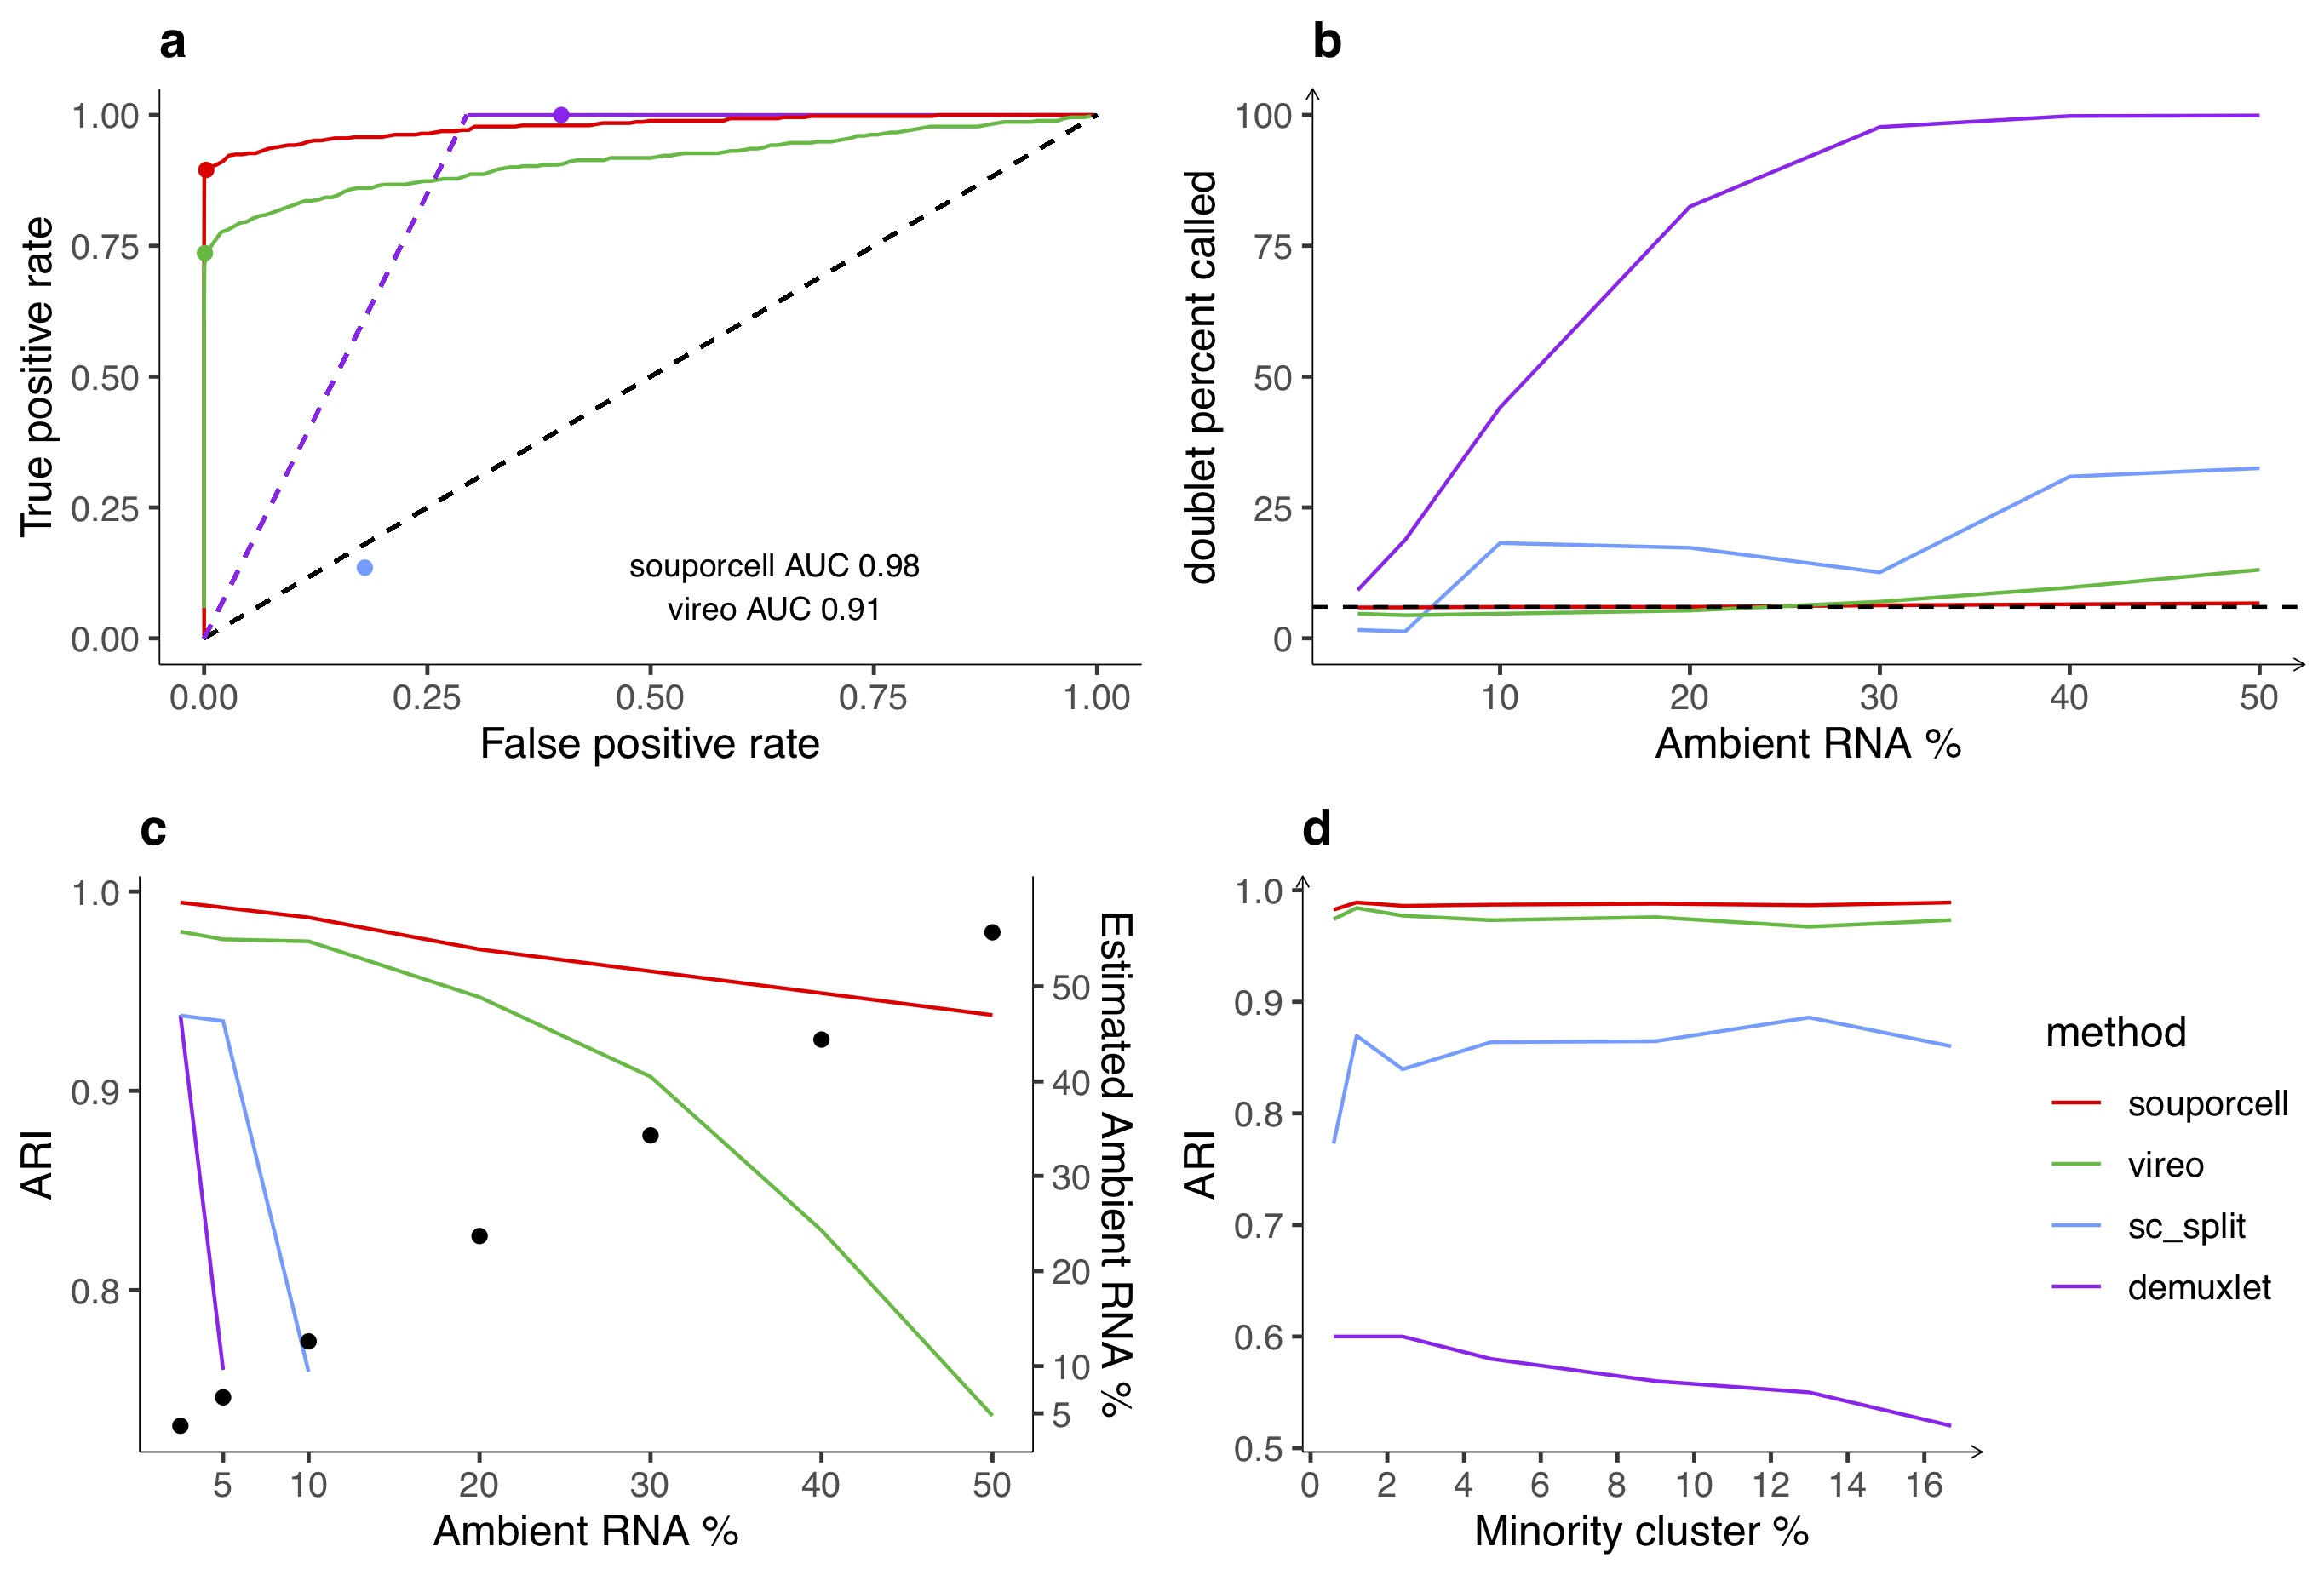
\includegraphics[width=\textwidth]{humcompare.jpg} 
\end{centering}
\floatfoot{\small{\textbf{a)} ROC curve of the doublet calls made by souporcell and vireo and a point estimate for scSplit (blue dot) for a synthetic mixture with 6\% doublets 451/7073 and 10\% ambient RNA. I show both the curves and the threshold chosen (points) for each tool. scSplit did not give a score so I simply show the point estimate. Demuxlet's doublet probabilities were all 1.0 until the solid line starts, so I show a theoretical dotted line up to that point. \textbf{b)} Doublet call percentages for all tools on synthetic mixtures for varying amounts of ambient RNA versus the actual doublet rate (dotted line). \textbf{c)} Adjusted Rand Index (ARI) versus the known ground truth of synthetic mixtures with 6\% doublets and a varying amount of ambient RNA. For levels >=10\% ambient RNA, scSplit identified one of the singleton clusters as the doublet cluster, which means that the ARI was not clearly interpretable. Right y-axis vs points shows the estimated ambient RNA percent by souporcell versus the simulated ambient RNA percent. \textbf{d)} ARI of each tool on a synthetic mixture with 8\% ambient RNA and 6\% doublet rate with 1,000 cells per cluster for the first four clusters and a variable number of cells in the minority cluster (25-800 cells in the minority cluster).}}
\end{figure}

\subsection{Maternal-Fetal data}

\par{
Next, we considered more challenging scenarios involving multiple cell types, widely varying numbers of cells per sample, and closely related genotypes. The decidua-placental interface plays an important role in pregnancy and birth, and is of importance to several diseases, including pre-eclampsia\cite{maternalfetal}. Recently, more than 70,000 cells were profiled by scRNAseq\cite{nkhla} to explore the transcriptional landscape at this interface. The decidua is primarily composed of maternal cells with some invading fetal trophoblasts, while the placenta is largely composed of cells of fetal origin with the exception of maternal macrophages. In the study exploring this interface\cite{maternalfetal}, WGS from blood and placenta was used to genotype both mother and fetus, and demuxlet was used to assign cells to each individual. Here, I applied souporcell, vireo, and scSplit to two placental samples and one decidual sample from a single mother to determine if cellular origins could be established without reference genotypes. I show the expression t-SNE of a single placental sample labeled by cell type annotation\cite{maternalfetal} and colored by genotype cluster as assigned by each method (\ref{figure:maternal}). While souporcell clusters agree with demuxlet and segregate with the expected cell type clusters, vireo and scSplit have major discordances with demuxlet. This is similar for the other samples tested. Comparing souporcell to demuxlet, there are 21 cells that demuxlet labels as maternal or fetal but which appear in the other individual's cell type clusters. Based on the position of these cells in the expression t-SNE plot, it is most likely that these are errors in the demuxlet assignments that are not made by souporcell. 
}


\begin{figure}[htbp!]
\caption{Maternal/fetal data}
\label{figure:maternal}
\begin{centering}

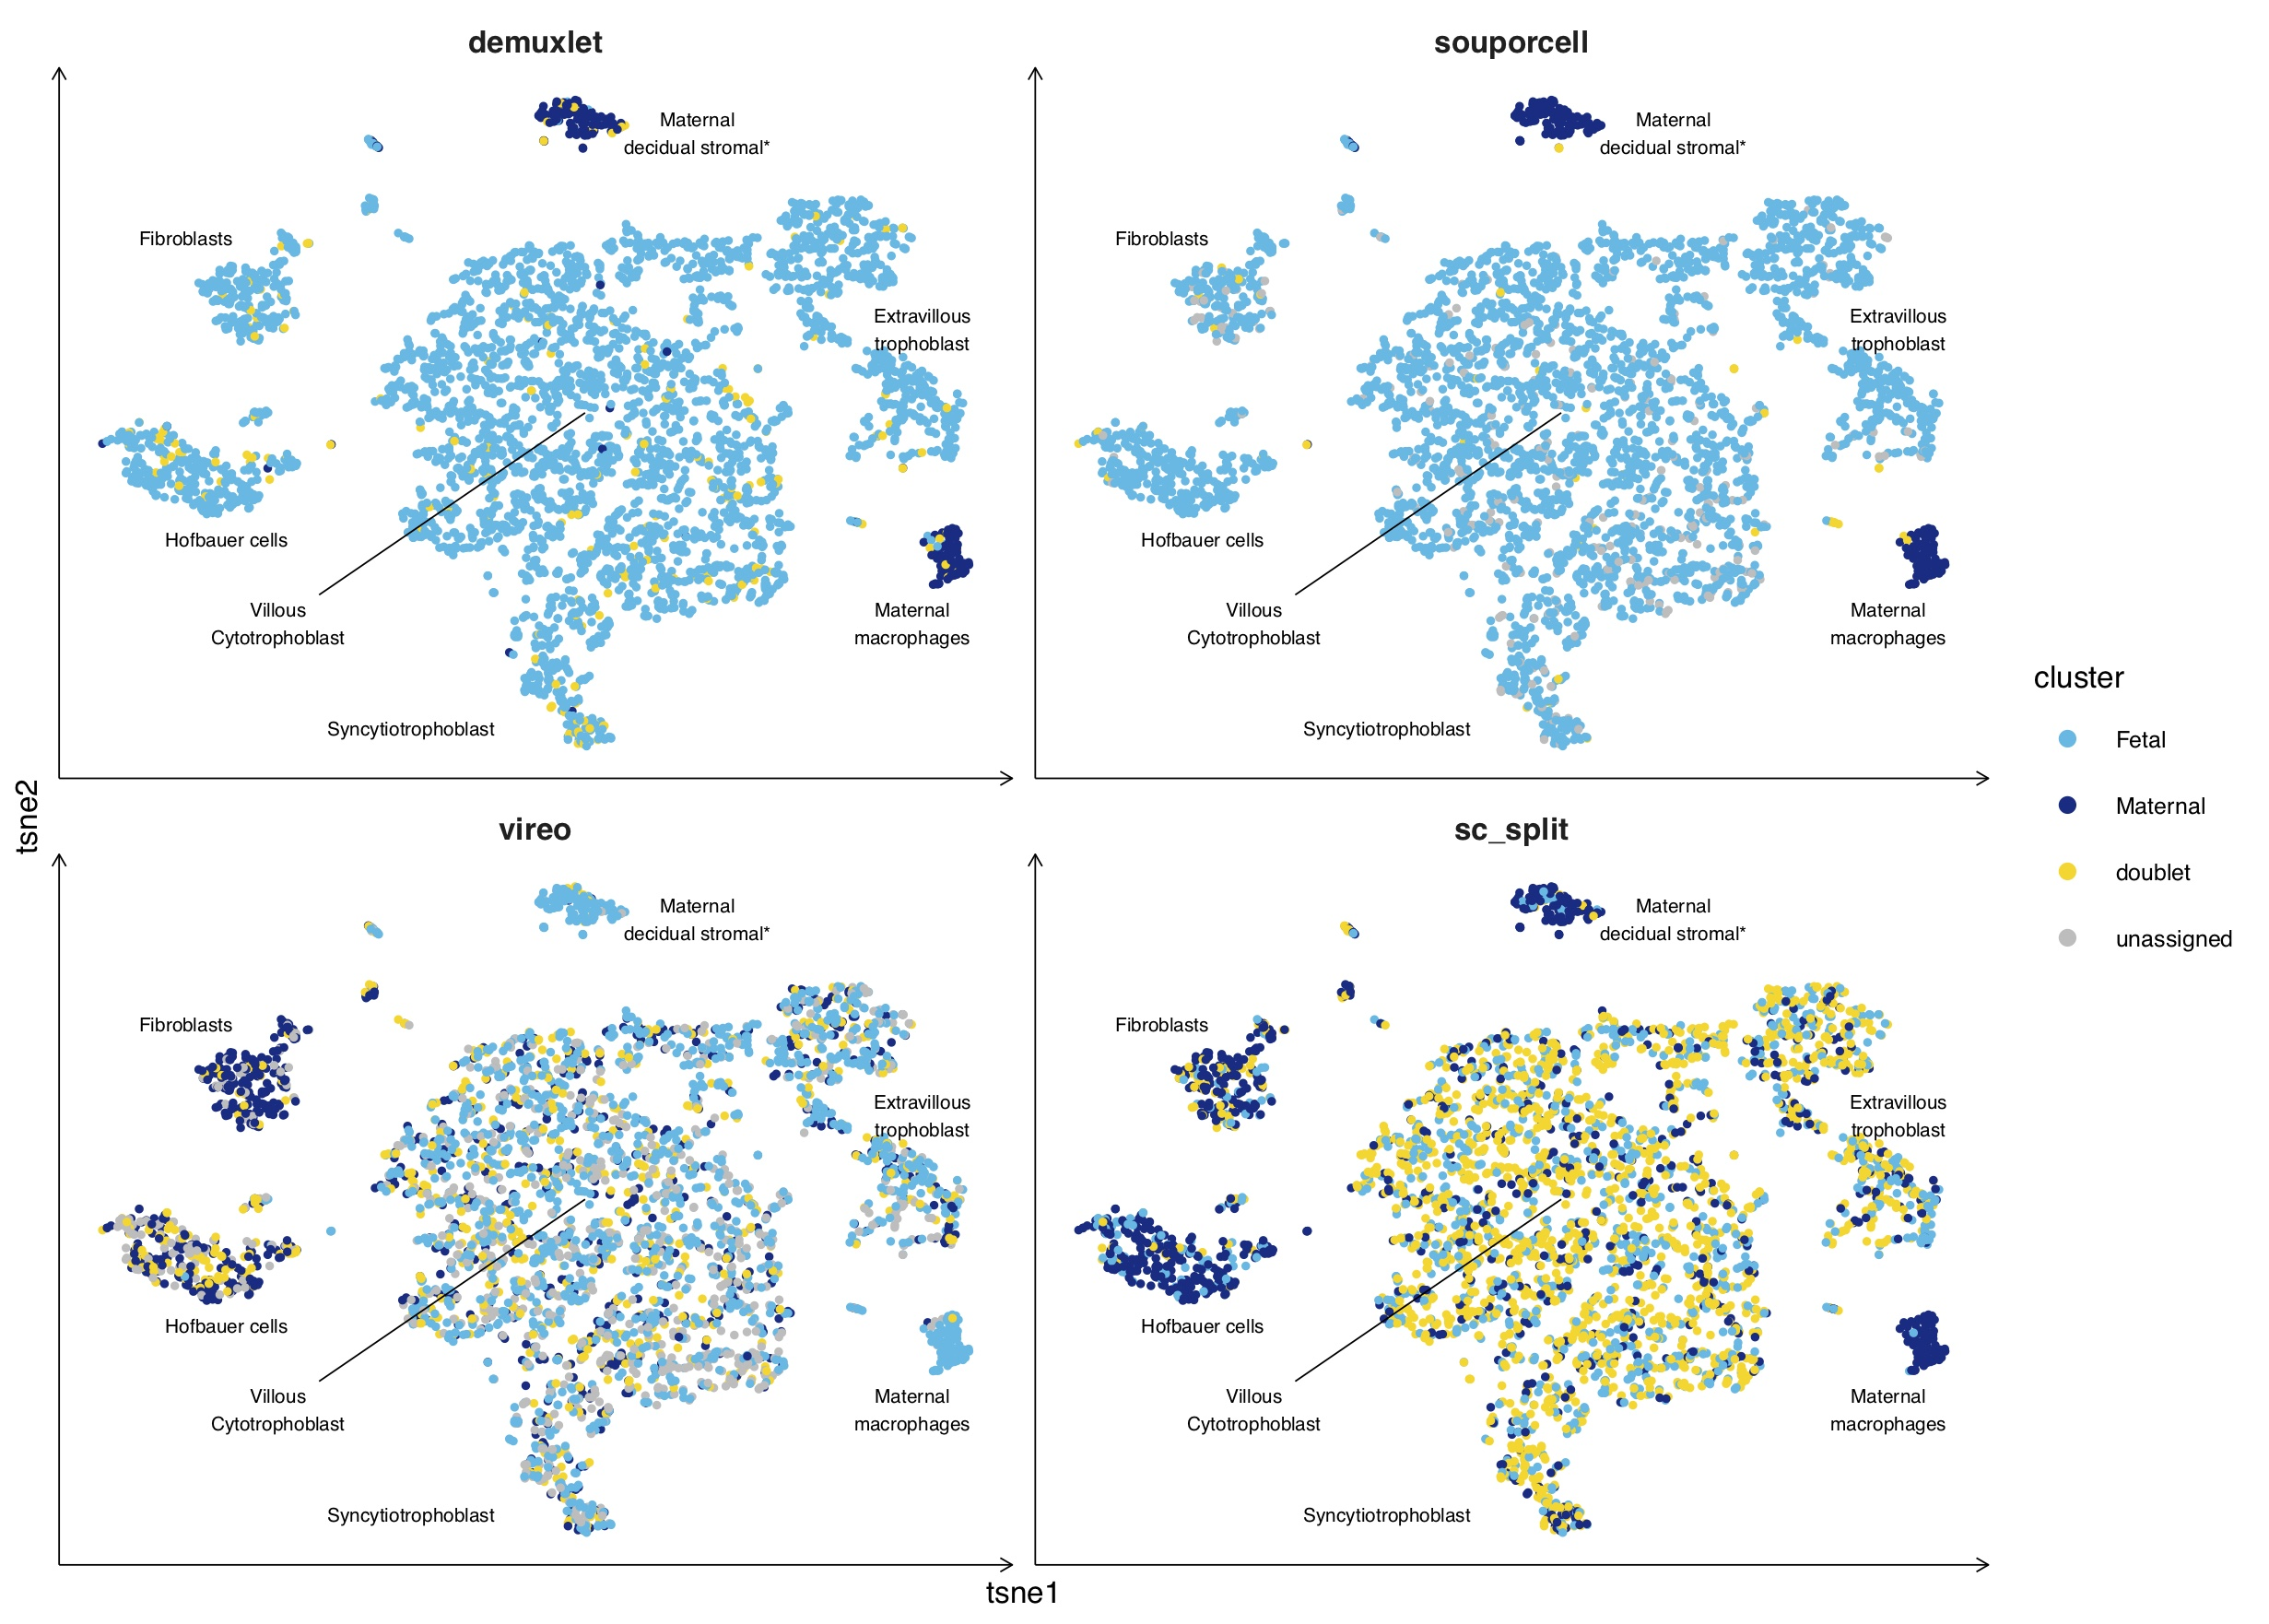
\includegraphics[width=\textwidth]{maternal.jpg} 
\end{centering}
\floatfoot{\small{Cell expression t-SNE plots of n=3,835 cells colored by each tool's genotype assignments or clusters for a placental sample. Cell phenotype clusters and cell genotype clusters co-segregate, with the majority of cell types being of fetal origin with the exception of maternal macrophages and *maternal decidual stromal cells, the latter of which (found only in one donor) were considered to be a non-placental artefact arising from the surgical procedure and were removed during data quality control in the original study\cite{maternalfetal}. Concordance is high between souporcell and demuxlet (ARI 0.96) whereas vireo and scSplit have large discordances with ARI of 0 and 0.03 respectively.}}


\end{figure}


\subsection{Plasmodium}

\begin{figure}[htbp!]
\caption{Plasmodium data}
\label{figure:malaria}
\begin{centering}
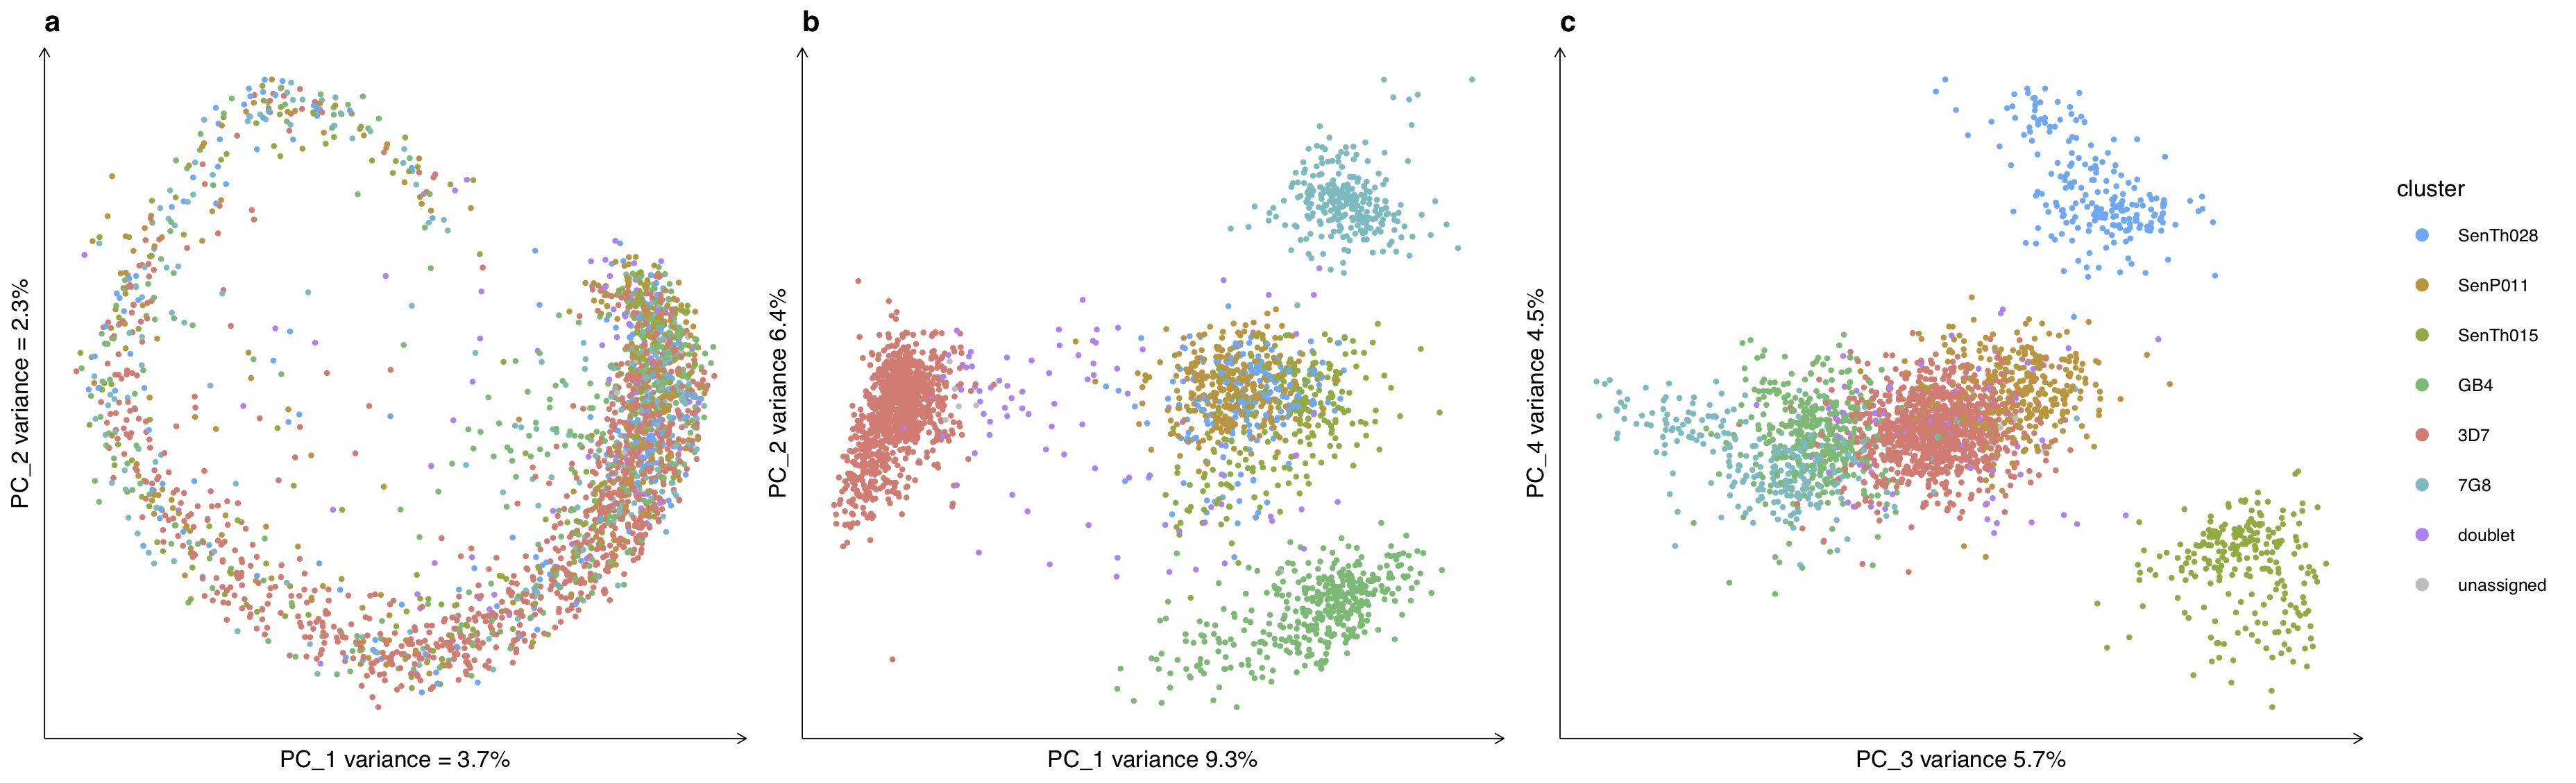
\includegraphics[width=\textwidth]{malaria.jpg} 
\end{centering}
\floatfoot{\small{\textbf{b)} Expression PCA colored by genotype clusters for Plasmodium sample 1 (n=2608 cells) (other samples in Fig. S3) showing an even spread of genotypes throughout the asexual lifecycle. \textbf{b} and \textbf{c)} PCAs of first four PCs of souporcell's normalized cell-by-cluster loss matrix showing good separation of each genotypic cluster (n=2608 cells).}}
\end{figure}

\par{
I also tested souporcell on a non-human sample, the single-celled malaria parasite \textit{Plasmodium falciparum}, for which single cell approaches are now used to explore natural infections\cite{MCA}. Malaria infections often contain parasites from multiple different genetic backgrounds, and it is not possible to separate the strains prior to sequencing. These samples differ from human samples in a variety of ways; they are haploid when infecting humans, the genome is $>80$\% A/T, and the transcriptome is only $\sim12$ megabases (genome is $\sim23$ Mb). We generated three datasets containing six genetically distinct strains of \textit{P. falciparum} (methods) sampling 1893-2608 cells with median UMIs of ~1000. Analysis of the expression profile of one of these (see Fig. S3 for the others) reveals that the genotypes are distributed across the \textit{Plasmodium} intra-erythrocytic cycle (\ref{figure:malaria}a) while being well separated in normalized loss cluster space (\ref{figure:malaria}b,c). The ARI for each method on the three \textit{Plasmodium} data sets show superior performance for souporcell across the board, with scSplit suffering on all datasets and vireo performing poorly on one, which had an ARI versus demuxlet of 0.24. This sample was more difficult due to sample skew caused by a clonal expansion of one of the six strains.
} 

\par{
We did three \textit{Plasmodium falciparum} mixture experiments. In the one shown above, the cells were mixed and immediately prepared for single cell sequencing. In the second one, the cells were mixed and then fixed in methanol before being prepared for scRNAseq. In the third mixture, cells were mixed and then grown in culture for seven days prior to single cell sequencing. Because the initial mixture was not very equal, the majority strain out grew the other strains dramatically. This caused the number of cells from some of the other strains to contain very few cells and be more difficult to cluster. Figure \ref{figure:malaria_replicates} shows the results of the 2nd and 3rd mixtures. The Plasmodium 3 sample which was cultured for seven days prior to being sequenced did not cluster into six clusters well. The elbow plot seemed to support a K of 3 more than the true number of strains mixed. This shows some of the limitations of souporcell and clustering in general with highly skewed number of cells per sample.
}


\begin{figure}[htbp!]
\caption{Plasmodium data replicates}
\label{figure:malaria_replicates}
\begin{centering}

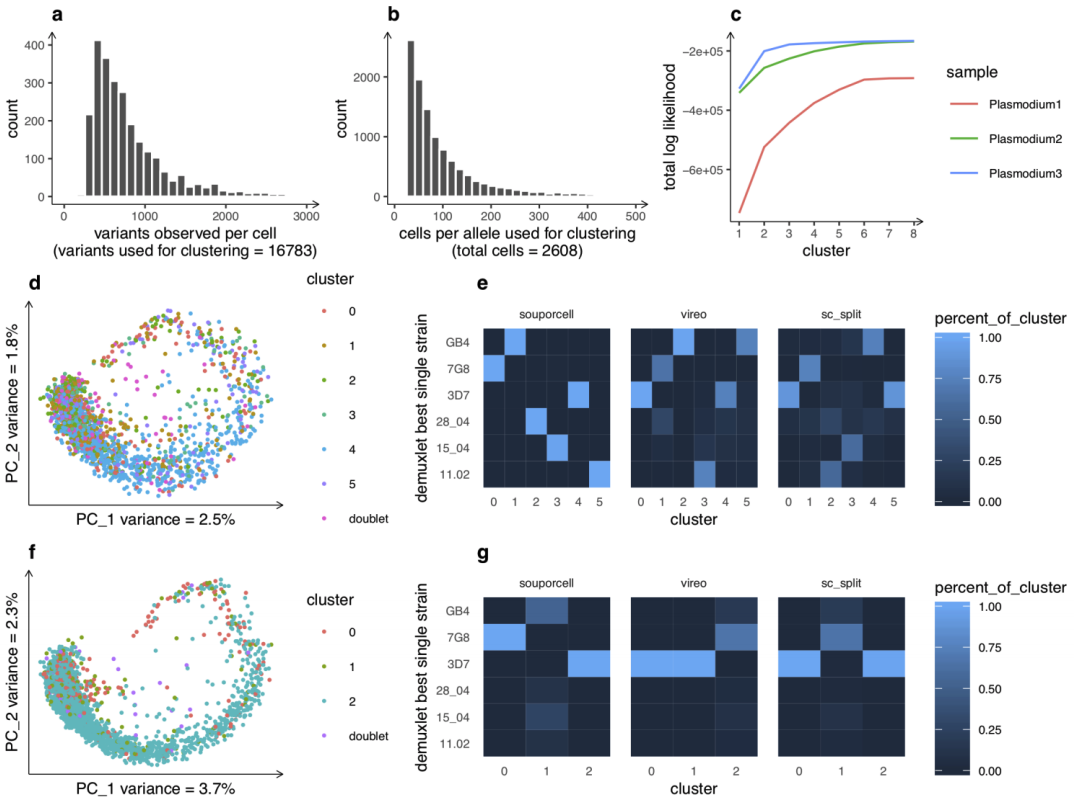
\includegraphics[width=\textwidth]{plasmodium_replicates.jpg} 
\floatfoot{\small{\textbf{a)} Distribution of number of variants observed per cell used for clustering (with at least 4 cells required to support each allele) and the
total number of variants used for clustering on the Plasmodium1 sample. \textbf{b)} Distribution of counts of the number of cells expressing
each allele used for clustering as well as the total number of cells in the Plasmodium1 sample. \textbf{c)} Elbow plots for each Plasmodium
data set show relatively strong support for the correct number of clusters (6) for Plasmodium1, but less clear results for Plasmodium2,
which suffered from higher amounts of ambient RNA, and for Plasmodium3, which due to more cell numbers biased towards three
genotypes rather than a relatively even mixture. For this reason, I analyzed Plasmodium3 with k=3. \textbf{d)} Expression PCA of the
Plasmodium2 sample (1893 cells) colored by genotype clusters as called by souporcell. \textbf{e)} Confusion matrix heatmap of the demuxlet
best single strain (Y axis) versus souporcell, vireo, and scSplit. For souporcell one cluster per strain is seen as expected. Both vireo
and scSplit have the majority strain, 3D7, split across two clusters and two other strains combined into a single cluster. \textbf{f)} Expression
PCA of the Plasmodium3 sample (2293 cells) colored by genotype clusters as called by souporcell. \textbf{g}) Confusion matrix heatmap of the
demuxlet best single strain (Y axis) versus souporcell, vireo, and scSplit genotype clusters with k=3. Souporcell clusters out the 3D7
and 7G8 strains correctly and puts all other cells into the final cluster while both vireo and scSplit put 3D7 into two clusters and all other
cells into the remaining cluster.}}

\end{centering}
\end{figure}




\subsection{Twenty one individual mixture demonstration}
\par{
I demonstrate that souporcell is capable of demultiplexing many donors by creating a synthetic mixture
of 21 different individuals, which given the current recommendations from 10x on cells per run would be
a high-end number of donors to multiplex. To generate this 21-donor mix, I used the 5 HipSci samples
described in \ref{figure:synthetic} and added to them 16 PBMC samples obtained from the Human Cell Atlas Census of
Immune Cells. From each dataset I randomly selected 1000 cells with at least 4000 UMIs and
simulated 10\% doublets and 2.5\% ambient RNA by altering the cell barcodes, as described above. I
clustered these with souporcell and the software correctly identifies 1690 of the 2100 synthetic doublets.
A further 69 cells were unassigned, and in total has an ARI of 0.95. Excluding all doublets the ARI
is 0.98. I found that a total of 134/16800 singletons misassigned where 129 of them are CB8 cells assigned to
the CB3 cluster. I show later that this is likely because the CB8 sample is contaminated by another
(non CB3) donor. \ref{figure:21donor} shows the UMAP projection of the normalized cluster log likelihood
matrix. It is clear that souporcell is able to handle at least 21 distinct donors and accurately assign cluster
identities to the majority of cells. 
} 

\par{
Because this error type accounted for >95\% of singleton errors, we suspected this may be due to
contamination. I repeated this experiment with several of the replicates of the CB8 donor and found
consistent results. I then made a synthetic mixture of CB3 and CB8 in order to determine if this was
due to the large number of donors and it was not. I still found that roughly 20\% of CB8 cells would
cluster with CB3, but if given 3 clusters, all of those cells formed their own cluster. This made us suspect 
that the CB8 sample was contaminated with cells from a different (non CB3) donor.
}


\begin{figure}[htbp!]
\caption{21 donor example}
\label{figure:21donor}
\begin{centering}

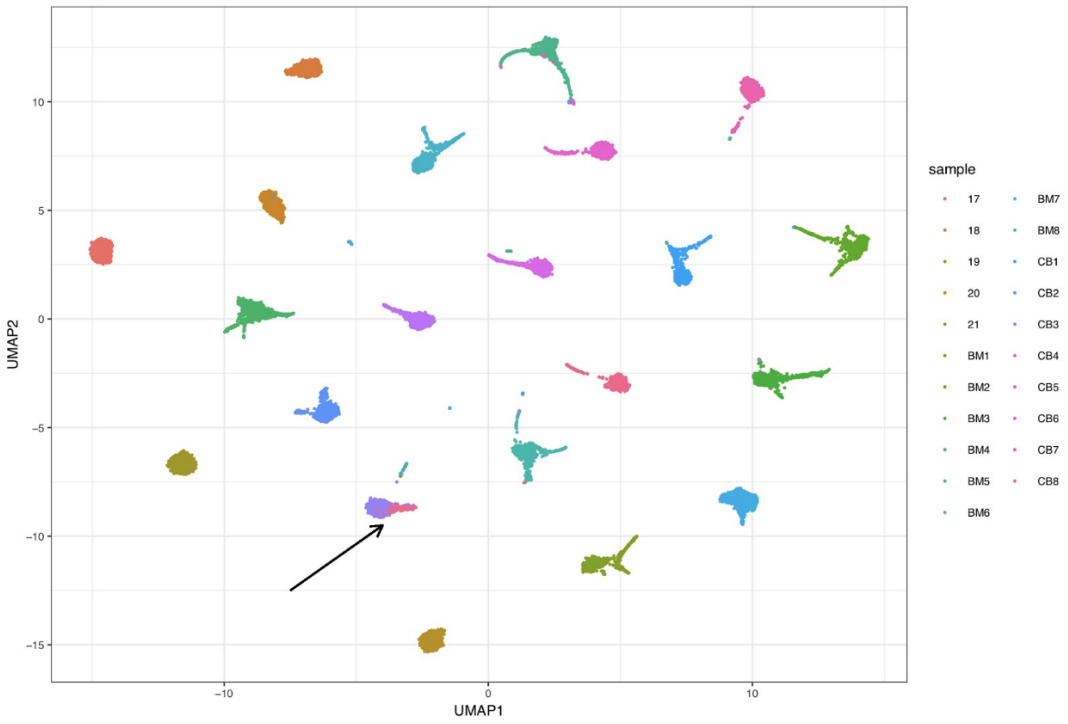
\includegraphics[width=\textwidth]{21donor.png} 
\end{centering}
\floatfoot{\small{UMAP of the normalized log likelihood cluster matrix for the singletons of a mixture of the 5 HipSci samples and the 16 PBMC
samples from the Human Cell Atlas project. The main error is the assignment of 129 CB8 cells to the CB3 dominant cluster indicated by
the arrow. I show later that this is likely due to contamination.}}


\end{figure}

\subsubsection{Contamination revealed}

\par{
To further test whether the CB8+CB3 ``misassignment'' was an error or true signal, I created a synthetic mixture of all cells from both the CB8 sample and the CB3 sample. I ran souporcell with a range of $K$ from 1 to 5 and plotted the elbow curve \ref{figure:contamination}a and the PCA of the cell cluster likelihoods for the clearly optimal number of clusters which was three. This PCA has good separation and gives good evidence that the CB8 sample was contaminated with cells from another donor which were most likely more closely related to the CB3 sample than the CB8 sample. I followed up with the creators of the census of immune cells data resource and they said that they were already aware of a contamination in the CB8 sample. This corroborated discovery was not picked up by the vireo team which used the same data with which they reported high concordance. This shows further the power of souporcell for detection of unexpected events such as sample contamination.
}

\begin{figure}[htbp!]
\caption{Contamination revealed}
\label{figure:contamination}
\begin{centering}

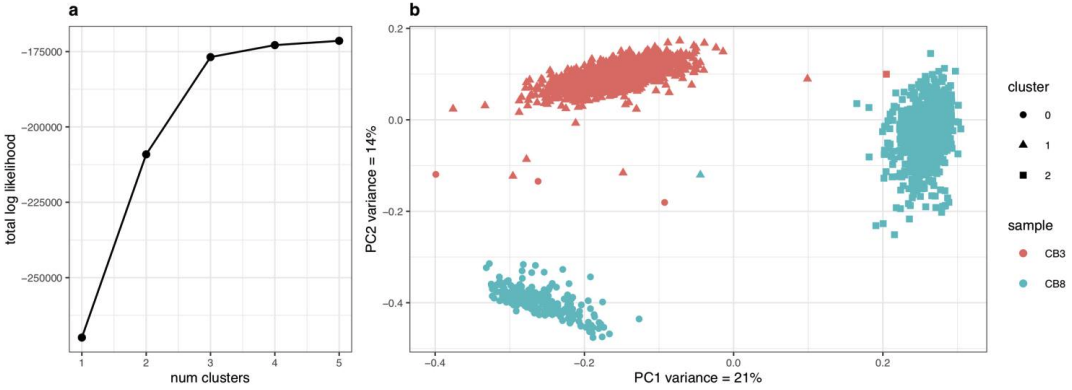
\includegraphics[width=\textwidth]{contamination.png} 
\end{centering}
\floatfoot{\small{\textbf{a)} Elbow plot of CB8+CB3 synthetic mixture with 3\% doublets shows a clear preference for three clusters rather than the expected two.
\textbf{b)} Shows the PCA of the normalized cell by cluster log likelihood matrix (n=2716 cells) showing three distinct genotypes.}}


\end{figure}

\subsubsection{Downsampling experiments for cells and UMIs}
\begin{figure}[htbp!]
\caption{Performance on low UMI counts}
\label{figure:umidown}
\begin{centering}

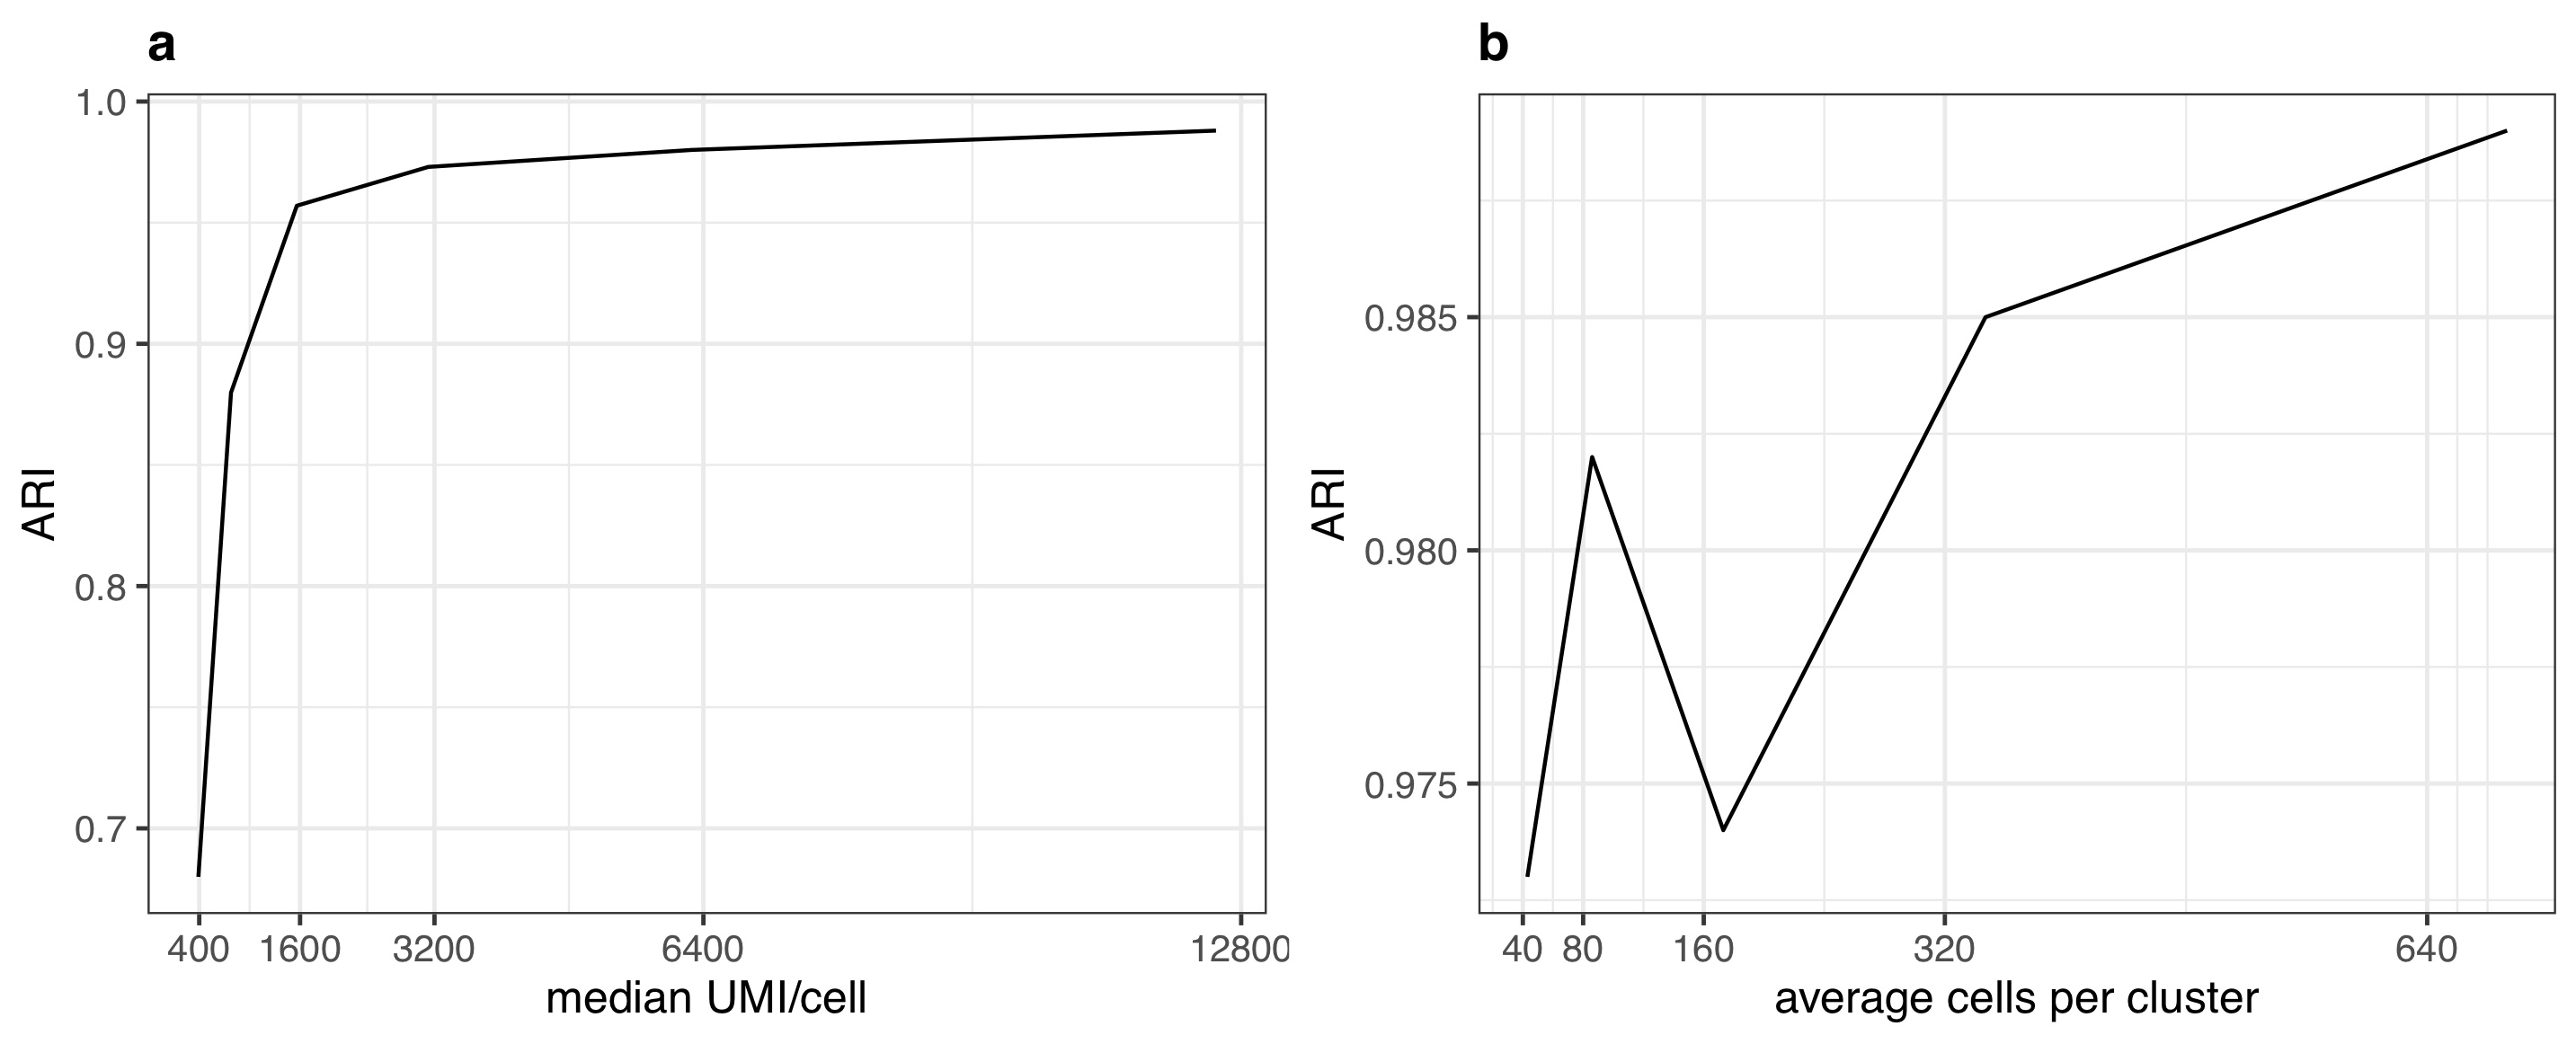
\includegraphics[width=\textwidth]{umidown.jpg} 
\end{centering}
\floatfoot{\small{\textbf{a)} The synthetic mixture of 5 HipSci cell lines with 6\% doublets and 5\% ambient RNA with UMIs downsampled shows predominantly
good clustering, but performance drops below 800 UMIs/cell. \textbf{b)} The clustering is consistently good with downsampled cells down to an
average cell per cluster of 40. The cluster with the fewest cells in the 40 average cells per cluster had 20 cells.}}


\end{figure}

\par{
In order to explore the regime for which it is still possible to accurately demultiplex mixed samples, I
used our synthetically mixed 5 HipSci samples and downsampled UMIs (figure \ref{figure:umidown}a) and cell (figure \ref{figure:umidown}
b) and report the ARI versus the ground truth. I found that while overall clustering remains good, cell
assignment accuracy decreases below 800 median UMI per cell and that accuracy remains high down to
an average of 40 cells per cluster (see figure \ref{figure:umidown}b). 
}






\section{Discussion}
\par{
Here I have presented souporcell, a method for clustering scRNAseq cells by genotype using sparse mixture model clustering with explicit ambient RNA modeling. Our benchmarks show that souporcell can outperform all other currently available methods, including those that require genotypes \textit{a priori}. Using more realistic and challenging test cases than previous studies, I show that souporcell is robust across a large range of parameters, and more so than any other currently available method. Moreover, souporcell is highly accurate for challenging datasets involving closely related maternal/fetal samples, and varying mixtures of Plasmodium falciparum strains. Limitations of souporcell include low signal to noise due to decreased UMI per cell and high numbers of donors causing increased local maxima. Due to the advantages that mixtures give to scRNAseq experiments in ameliorating batch effects, improving doublet detection, and allowing for ambient RNA estimation, souporcell enables donor multiplexing designs to be used more easily than was previously possible, including in situations when no WGS or genotyping data are available. In addition to reducing cost and allowing for more complex and robust experimental designs, souporcell also enables valuable genotype information to be extracted and ambient RNA estimation at no additional cost.
}

%********************************** % Third Section  *************************************


%!TEX root = ../thesis.tex
%*******************************************************************************
%****************************** Third Chapter **********************************
%*******************************************************************************
\chapter{High quality assembly of a single Mosquito}

% **************************** Define Graphics Path **************************
\ifpdf
    \graphicspath{{Chapter3/Figs/Raster/}{Chapter3/Figs/PDF/}{Chapter3/Figs/}}
\else
    \graphicspath{{Chapter3/Figs/Vector/}{Chapter3/Figs/}}
\fi



\section{Background}
\par{
Exciting efforts to sequence the diversity of life are building momentum \cite{Lewin2018-lc} but one of many challenges that these efforts face is the small size of most organisms. For example, arthropods, which comprise the most diverse animal phylum, are typically small. Advances in long read sequencing over the past decade have revolutionized genome assembly and reference genome creation\cite{pacbio}\cite{oxford}, but until recently the DNA requirements for these technologies were relatively high. This made long read sequencing of single individuals impossible for many small species due to the amount of DNA that can be extracted even when consuming the whole specimen. In the standard assembly process, when considering sequences which have inexact homology, you must decide whether the differences arose from errors, haplotype differences, or paralogous sequences. If it is determined that the differences are due to heterozygosity, an assembler would collapse the sequence. However, if the assembler decides the sequences are repeats and thus represent different locations (close or distal) in the genome, they should be assembled separately (see figure \ref{figure:assembly}). As the haplotype differences increase, it reduces the assembler's ability to distinguish paralogous sequences from haplotype differences for higher divergent repeats. When you cannot distinguish these processes and no reads span the repeat (and if it is due to haplotype differences, no reads will span as the homology is highly likely to continue), the contig must end to avoid chimeric misassemblies. This results in fractious and error prone genome assemblies. One could, of course, pool multiple individuals together to meet the DNA requirements, but this has serious downsides. Using a pool of individuals increases the number of haplotypes being sequenced and increases the expected haplotype differences which reduces your ability to distinguish paralogous sequences from haplotype variation. Moreover, the structural variation in the pool of haplotypes can cause further problems in assembly. These problems are accentuated in these small species that require pooled long read sequencing, because, while levels of heterozygosity within species vary widely across taxa, intraspecific genetic variation is often highest in small organisms \cite{Leffler2012-uh}. 
}

\begin{figure}[htbp!]

\begin{centering}
\caption{Assembly of inexact homologous sequences: heterozygosity vs paralogous sequences}\label{figure:assembly}

\sidesubfloat[]{
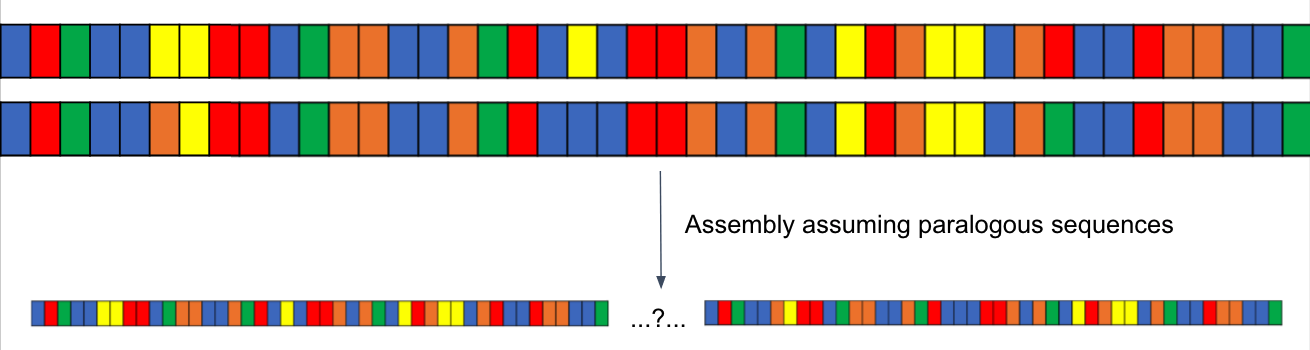
\includegraphics[width=0.95\textwidth, valign=t]{paralogues.png} \label{fig:a}
} \\
\sidesubfloat[]{
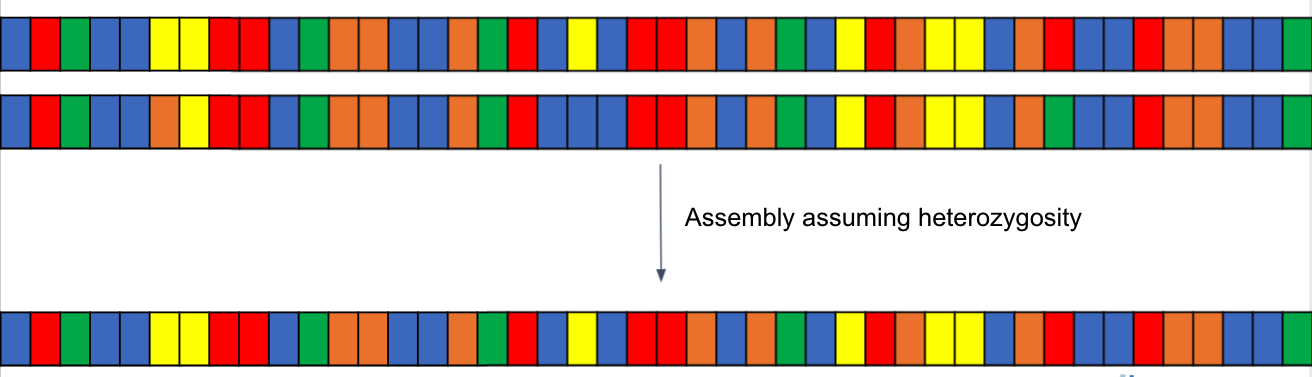
\includegraphics[width=0.95\textwidth, valign=t]{heterozygous.png} \label{fig:b}
}

\par{Inexact homologous sequences and how they would be assembled if the differences are due to \textbf{a)} paralogous sequences or \textbf{b)} heterozygous differences. }
\end{centering}
\end{figure}


\par{
To address these problems, over the past two decades, reference genomes for many small organisms have been built through considerable efforts of inbreeding organisms to reduce their heterozygosity levels such that many individuals can be pooled together for DNA extractions with more similar haplotypes. This approach has varied in its success, for example working well for organisms that are easy to inbreed (e.g., many \textit{Drosophila} species \cite{Drosophila_12_Genomes_Consortium2007-fx}), but less well for species that are difficult or impossible to inbreed (e.g., \textit{Anopheles} \cite{Neafsey2015-op}). Therefore, many efforts to sequence genomes of small organisms have relied primarily on short-read approaches due to the large amounts of DNA required for long read sequencing. For example, the recent release of 28 arthropod genomes as part of the i5K initiative used four different insert size Illumina libraries, resulting in an average contig N50 of 15 kb and scaffold N50 of 1 Mb \cite{Thomas2018-rk}.
} \\

\par{
Another way to overcome DNA input requirements, while also reducing the number of haplotypes present in a DNA pool, is to limit the number of haplotypes in the pool of individuals by using offspring from a single cross. This is easier than multiple generations of inbreeding, and can be successful. For example, a recent PacBio \textit{Aedes aegypti} assembly used DNA extracted from the offspring of a single cross, thus reducing the maximum number of haplotypes for any given locus to four, thereby improving the assembly process and achieving a contig N50 of 1.3 Mb \cite{Matthews2018-th}. These four haplotypes will have recombined with each other in the cross, but recombinations are fairly rare and do not greatly increase the haplotype differences problems in assembly. Even this may run into problems though. For example, in species which mate multiple times and store sperm in a spermatheca as is the case in many diptera\cite{spermatheca}\cite{polyandry} it may be difficult to create a pure single cross. Also, these are not conducive to wild-caught organisms and must be grown in a lab for controlled crossing.
} \\

\par{
However, for an initiative like the Earth BioGenome Project \cite{Lewin2018-lc} that aims to build high-quality reference genomes for more than a million described species over the next decade, generating broods to reach sufficient levels of high molecular weight DNA for long-read sequencing will be infeasible for the vast majority of organisms. Therefore, new methods that overcome the need to pool organisms are needed to support the creation of reference-quality genomes from wild-caught individuals to increase the diversity of life for which reference genomes can be assembled. Here, we present the first high-quality genome assembled with unamplified DNA from a single individual insect using a new workflow that greatly reduces input DNA requirements. Until recent advances in long read library preparation \cite{mosquito_assembly}, it was not possible to obtain
enough DNA from a single individual of small organisms such as mosquitos to create a long read sequencing library from one individual. 
But for many other smaller species, this still remains the case. And it also remains the case for nanopore sequencing. 
Whether it is possible to decrease the input requirements for nanopore sequencing and to what extent are currently unknown.  
} \\

\par{
In this chapter we discuss the process of making the first high quality assembly of a single mosquito and assess its quality and completeness. We first discuss the methods used for high molecular weight (HMW) DNA extraction and resulting length profiles. The extraction was done at the Sanger Institute, but the sequencing was done in California. So a further length profile is included to show the DNA length degradation from transit. We then discuss the new low input library prep and the sequencing used. We outline briefly the curation steps taken which resulted in changes to the assembly before going through each analysis in detail. Assembly quality is then assessed first through comparison of contiguity of the assembly and curated assembly against the current gold standard reference genome (Agam4 PEST). Next completeness and assembly duplication are inspected via comparing to known orthologous gene sets with BUSCO (Benchmarking Universal Single-Copy Orthologs). Finally, we do a series of genome comparisons to the PEST reference. In this, we are able to identify and correct a misassembly and uncover significant remaining duplicated haplotype assembly sequence and its cause. In this analysis, we are also able to find many improvements our assembly makes over the PEST assembly including placing of previously unplaced genes in their chromosomal context. We also dramatically reduce the assembly gaps. We find significant evidence of collapsed complex repeats in PEST that have been accurately expanded in our assembly. We then find an order-and-orientation error in the PEST reference. Finally, we show the contig coverages of the PEST reference aligned to the PacBio assembly and how much of the UNKN contigs are likely haplotigs and visually show the placement of other UNKN sequence.
} \\

\par{
The genome we use for comparison was built using bacterial artificial chromosomes (BACs) and Sanger sequencing, the same basic technology initially used to create the human reference genome, which is highly accurate but extremely labor intensive and expensive. Our assembly allows for the use of a single individual, is relatively cheap, and is more accurate and complete than the previous gold standard \textit{Anopheles} genome. With some addition data, or by scaffolding against the PEST reference as shown in this chapter, it would also be more contiguous with fewer gaps.
}

\section{DNA Isolation}

The DNA isolation was carried out by Juliana Cudini, a fellow PhD student. \\

\par{
High molecular weight (HMW) DNA was isolated from a single \textit{Anopheles coluzzii} female from the Ngousso colony. This colony was created in 2006 from the broods of approximately 100 wild-caught pure \textit{Anopheles coluzzii} females in Cameroon (pers. comm. Anna Cohuet). Although the colony has been typically held at >100 breeding individuals, given the long time since colonization, there is undoubtedly inbreeding. A single female was ground in 200 $\mu l$ PBS using a pestle with several up and down strokes (i.e., no twisting), and DNA extraction was carried out using a Qiagen MagAttract HMW kit (PN-67653) following the manufacturer's instructions, with the following modifications: 200 $\mu l$ 1X PBS was used in lieu of Buffer ATL; PBS was mixed simultaneously with RNAse A, Proteinase K, and Buffer AL prior to tissue homogenization and incubation; incubation time was shortened to 2 h; solutions were mixed by gently flicking the tube rather than pipetting to reduce shearing and maximize extracted DNA length; and subsequent wash steps were performed for one minute. Any time DNA was transferred, wide-bore tips were used. These modifications were in accordance with recommendations from 10X Genomics HMW protocols that aim to achieve >50 kb molecules. The resulting sample contained ~250 ng of DNA, and we used the FEMTO Pulse to examine the molecular weight of the resulting DNA. This revealed a relatively sharp band at ~150 kb (figure \ref{figure:fempto2}). The DNA was shipped from the U.K. to California on cold packs, and examined again by running 500 pg on the FEMTO Pulse. While a shift in the molecular weight profile was observed as a result of transport, showing a broader DNA smear with mode of ~40 kb (figure \ref{figure:fempto}), it was still suitable for library preparation (note that this shifted profile is coincidentally similar to what is observed with the unmodified MagAttract protocol). DNA concentration was determined with a Qubit fluorometer and Qubit dsDNA HS assay kit, and 100 ng from the 250 ng total was used for library preparation.
}


\begin{figure}[htbp!]
\caption{\textit{Anopheles coluzzii} single mosquito HMW DNA extraction}
\label{figure:fempto2}
\begin{centering}
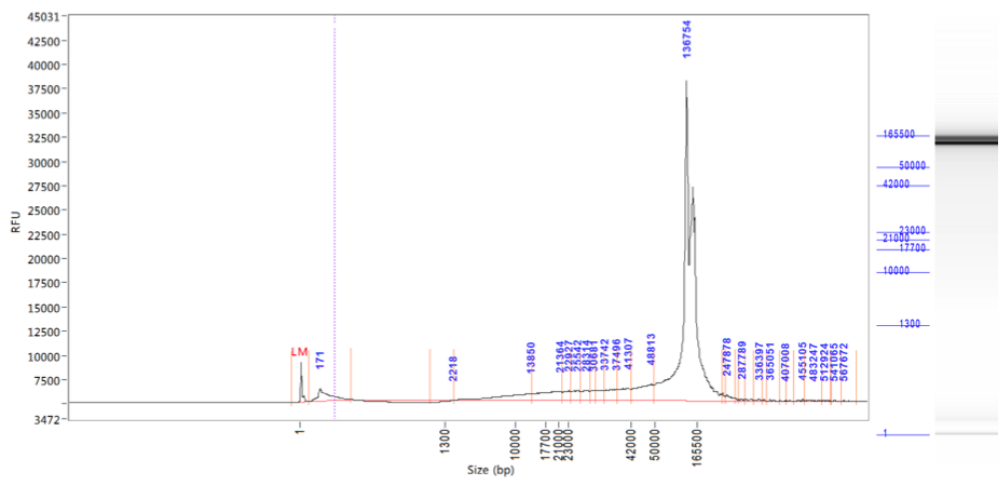
\includegraphics[width=.85\textwidth]{fempto2.png}
\par{ Femto Pulse evaluation of the Modified MagAttract DNA extraction prior to shipment to
California. }
\end{centering}
\end{figure}

\section{Library prep and Sequencing}

Library prep and sequencing were performed by Sarah Kingan, Senior Scientist at PacBio. \\

\par{
A SMRTbell library was constructed using an early access version of SMRTbell Express Prep kit v2.0 from Pacific Biosciences (PacBio). Because the genomic DNA was already fragmented with the majority of DNA fragments above 20 kb (figure \ref{figure:fempto}), the sequencing library preparation protocol was modified to exclude an initial shearing step, which facilitated the use of lower input amounts, as shearing and clean up steps typically lead to loss of DNA material. After following the Express template preparation protocol, the final clean up step was simplified to just two AMPure purification steps to remove unligated adapters and very short DNA fragments. The size and concentration of the final library (figure  \ref{figure:fempto}) were assessed using the FEMTO Pulse and the Qubit Fluorometer and Qubit dsDNA HS reagents Assay kit, respectively. This resulted in a final library with a size distribution peak around 15 kb (figure \ref{figure:fempto}). 
}


\begin{figure}[htbp!]
\caption{\textit{Anopheles coluzzii} input and resulting library DNA lengths}
\label{figure:fempto}
\begin{centering}
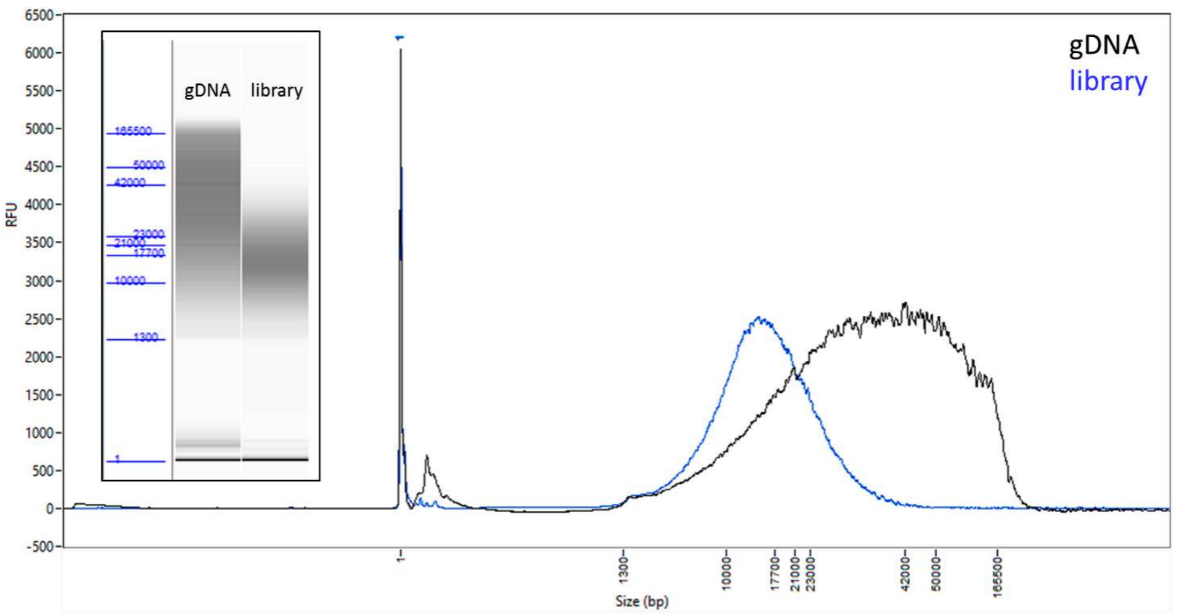
\includegraphics[width=.85\textwidth]{fempto.png}
\par{ FEMTO Pulse traces and gel images (inset) of the genomic DNA input (black) and the final library (blue) before sequencing. }
\end{centering}
\end{figure}

\par{
Sequencing primer v4 and Sequel DNA Polymerase 3.0 were annealed and bound, respectively, to the SMRTbell library. The library was then sequenced on the Sequel System with Sequel Sequencing Kit 3.0. 1200 minute movie with 120 minute pre-extension and Software v6.0. A total of three SMRT cells were run generating on average 24.2 Gb of data per SMRT Cell, with average insert lengths of 8.1 kb (insert length N50 \~13 kb, table \ref{table:dataamount}). This is double the standard exposure time allowing for more data out of the same sample. However, extending exposure times has diminishing returns. The overall library yield was 59\%, which would have allowed for the sequencing of at least 8 SMRT Cells, thereby potentially allowing for genome sizes 2-3 times larger or organisms that yield 2-3 times less DNA in extraction than studied here in conjunction with this protocol.
}

\begin{table}[htbp!]
\caption{Run statistics for Sequel SMRT Cells.}\label{table:dataamount}
\begin{tabular}{| c | c | c | c | c | c |}
\hline
Loading & Gb/cell & Mean  & N50 &  Mean &  N50  \\
concentration & & Polymerase & Polymerase & Subread & Subread \\
& & Read & Read & Length & Length \\ 
& & Length &Length & & \\\hline
5 pM & 24.1 & 40290 & 116615 & 8185 & 12978 \\\hline
5 pM & 23.6 & 40077 & 114807 & 8254 & 13132 \\\hline
6 pM & 25.0 & 47177 & 122898 & 8012 & 12751 \\\hline
\end{tabular}
\end{table}



\section{Assembly}

The assembly was run by Sarah Kingan, Senior Scientist at PacBio. My main role was in quality assessment and comparative genomics. \\

\par{
The genome was assembled using FALCON-Unzip, a diploid assembler that captures haplotype variation in the sample \cite{falcon}. A single subread per zero-mode waveguide (ZMW) was used for a total of 12.8 Gb of sequence from three SMRT Cells, or ~48-fold coverage of the ~266 Mb genome. Subreads longer than 4559 bp were designated as seed reads and used as template sequences for preassembly/error correction. A total of 8.1 Gb of preassembled reads was generated (~30-fold coverage). After assembly and haplotype separation by FALCON-Unzip, two rounds of polishing were performed to increase the consensus sequence quality of the assembly, aligning the PacBio data to the contigs and computing consensus using the Arrow consensus caller \cite{arrow}. The first round of polishing was part of the FALCON-Unzip workflow and used a single read per ZMW that was assigned to a haplotype. The second round of polishing was performed in SMRT Link v 6.0.0.43878, concatenating primary contigs and haplotigs into a single reference and aligning all subreads longer than 1000 bp (including multiple subreads from a single sequence read, mean coverage 184-fold) before performing genomic consensus calling. The alignments (BAM files) produced during the two rounds of polishing were used to assess confidence in the contig assembly in regions with rearrangements relative to the AgamP4 PEST assembly for \textit{Anopheles gambiae} (GenBank assembly accession GCA\_000005575.2) \cite{PEST}\cite{PEST2}. We referred to the first round of polishing as using unique subreads and the second round as using all subreads.
} \\

\par{
We explored the performance as a function of the number of SMRT Cells used for the assembly (table \ref{table:smrtcells}), and found that while a single SMRT Cell was insufficient to result in high-quality assembly, data from two or three SMRT Cells generated a highly contiguous assembly of the correct genome size. We proceeded with the three-cell assembly for all subsequent analyses because it gave the most contiguous and complete assembly results.
}

\begin{table}[htbp!]
\caption{Assembly quality vs the amount of data used.}\label{table:smrtcells}
\begin{tabular}{| c | c | c | c |}
\hline
 & \textbf{1 SMRT cell} & \textbf{2 SMRT cells} & \textbf{3 SMRT cells} \\\hline
 \textbf{Total bases (Gb)} & 23.6 & 48.5 & 72.7 \\\hline
  \textbf{Total unique bases (Gb)} & 4.46 & 8.31 & 12.8 \\\hline 
  \textbf{Unique coverage} & 17x & 31x & 45x \\\hline 
  \textbf{Assembly size (Mb)} & 150 & 265 & 271 \\\hline 
  \textbf{Number of contigs} & 3,290 & 815 & 580 \\\hline 
  \textbf{Contig N50 (Mb)} & 0.066 & 1.5 & 3.5 \\\hline
\end{tabular}
\par{Statistics for \textit{Anopheles coluzzii} de novo genome assemblies as a function of the number of
SMRT Cells used for the assembly. One cell failed to assembly the whole genome. Two and three cells assembled the majority of the genome but quality improved with 3 cells.}
\end{table}
%The resulting primary assembly consisted of 372 contigs totaling 266 Mb in length, with a contig N50 of 3.5 Mb and a secondary 
%haplotype assembly totalling 78.5 Mb. \ref{table:assemblydata} shows various assembly statistics of the long read assembly and the current 
%reference assembly of the closely related \textit{Anopheles gambiae}\cite{PEST}\cite{PESTupdate}\cite{PESTchromitin}\cite{gambiaeref}. 




\section{Curation}

\par{
The contigs were screened by the Sanger Institute and NCBI to identify contaminants and mitochondrial sequence \cite{sangercuration}. Windowmasker was used to mask repeats and the MegaBLAST algorithm was run (with parameter settings: -task megablast -word\_size 28 -best\_hit\_overhang 0.1 -best\_hit\_score\_edge 0.1 -dust yes -evalue 0.0001 -min\_raw\_gapped\_score 100 -penalty 5 -perc\_identity 98.0 -soft\_masking true -outfmt 7) on the masked genome versus all complete bacterial genomes to find hits with  greater than 98\% homology\cite{windowmasker}\cite{megablast}. One contig (\#20) was identified as a complete 4.24 Mb bacterial genome, closely related to \textit{Elizabethkingia anophelis}, which is a common gut microbe in Anopheles mosquitoes \cite{kingia}\cite{blobtoolkit}. It was separated from the mosquito assembly and submitted to NCBI separately. We also identified two contigs of mitochondrial origin that each contained multiple copies of the circular chromosome. Full length copies of the mitochondrial chromosome in the higher quality contig differed by only a single base and the consensus sequence was reported as the mitochondrial genome. One of these copies was discarded.
} \\

\par{
In addition, we screened the primary assembly for duplicate haplotypes using Purge Haplotigs \cite{purge} with default parameters and coverage thresholds of 20, 150, and 700. While FALCON-Unzip resolved haplotypes over ~30\% of the genome, 110 genes appeared as duplicated copies in the BUSCO analysis, indicating that highly divergent haplotypes may be assembled as distinct primary contigs as has been observed in other mosquito genome assemblies \cite{aegypti}\cite{funestus}. The presence of duplicated haplotypes can result in erroneously low mapping qualities in resequencing studies and cause problems in downstream scaffolding. Using the Purge Haplotigs software \cite{purge}, we identified 165 primary contigs totalling 10.6 Mb as likely alternate haplotypes, although there remains a possibility that some may be repeats. These contigs were transferred to the alternate haplotig set.
} \\


\par{
In the process of comparing the assembly to the PEST reference (described later), we found one large potential heterozygous interchromosomal rearrangement between 2L and 3R (see figure \ref{figure:misassembly}). Upon further exploration, this was not supported by any subreads mapping across the breakpoint (figure \ref{figure:misassembly}). The putative breakpoints were identified by aligning the PacBio contigs to PEST with minimap2 (asm5 setting)\cite{minimap2}, and the start and end position of each aligned subread was determined using bedtools bamtobed\cite{bedtools}. This 4.9 Mb contig had no reads spanning the putative breakpoint when either unique or all subread alignments were examined and thus we designated this a chimeric misassembly, and split the contig into two.
}



\section{Assembly quality assessment}


\par{
Using the FALCON-Unzip assembler\cite{falcon}, the resulting primary de novo assembly consisted of 372 contigs totaling 266 Mb in length, with half of the assembly in contigs (contig N50) of 3.5 Mb or longer (table \ref{table:assemblydata}). FALCON-Unzip also generated 665 alternate haplotigs, representing regions of sufficient heterozygosity to allow for the separation of the maternal and paternal haplotypes. These additional phased haplotype sequences spanned a total of 78.5 Mb (i.e., 29\% of the total genome size was separated into haplotypes), with a contig N50 of 223 kb (table \ref{table:assemblydata}). 
}


\begin{table}[htbp!]
\caption{Assembly statistics}\label{table:assemblydata}
\begin{center}
\begin{tabular}{ | l | l | l | l | l |}
\hline
\multicolumn{2}{|c|}{} & \textbf{Initial} & \textbf{Curated} & \textbf{PEST} \\
\multicolumn{2}{|c|}{} & \textbf{Assembly} & \textbf{Assembly} & \textbf{reference} \\
\hline
\multirow{3}{5em}{\textbf{Primary Assembly}}
& Size (Mb) & 266 & 251 & 224 \\
\cline{2-5}
& Number Contigs & 372 & 206 & 27,063 \\
\cline{2-5}
& Contig N50 (Mb) & 3.52	& 3.47	& 0.025 \\
\hline%\cline{2-5}
\multirow{3}{5em}{\textbf{Alternate Haplotigs}}
& Size (Mb) & 78.5 & 	89.2	& unresolved \\
\cline{2-5}
& Number Contigs & 665 &	830& 	N/A \\
\cline{2-5}
& Contig N50 (Mb) & 0.22	& 0.199	& N/A \\
\hline
\end{tabular}
\end{center}
\end{table}




\subsection{BUSCO analysis: completeness and duplication/haplotig retainment}

\par{
To evaluate genome completeness and sequence accuracy of the currated assembly, we performed alignment analyses to a set of conserved genes. Using the diptera set of the BUSCO (Benchmarking Universal Single-Copy Orthologs) gene collection, we observed 98\% of the ~2800 genes were complete and >95\% occurred as single copies (table \ref{table:busco}). By comparison, the previous assembly had 87.5\% complete BUSCO alignments, indicating that a fraction of the genome was missing in that assembly. The percentage of duplicated genes was reduced from 3.9\% to 2.4\% after curation.  Additional analyses are required to distinguish true gene duplication events from incomplete purging of duplicated haplotypes (see discussion below and figure \ref{figure:haplotig}). In addition, we evaluated assembly completeness against a curated set of genes (AgamP4.10 gene set) from the \textit{Anopheles gambiae} PEST reference, using a previously described script \cite{avian}. We aligned to the primary assembly a closely related species gene set (the most recent \textit{Anopheles gambiae} (AgamP4.10) gene set), resulting in 14,972 alignments (99.5\%) and an average alignment length of 96.6\%, and with >96\% of alignments showing no frame shift-inducing indels.
}


\begin{table}[htbp!]
\caption{BUSCO analysis.}\label{table:busco}
\begin{tabular}{| c | c | c | c |}
\hline
 \textbf{Gene count (\%)} & \textbf{Initial} & \textbf{Curated} & \textbf{PEST} \\\hline
   & \textbf{Assembly} & \textbf{Assembly} & \textbf{Reference} \\\hline
 \textbf{Complete} & 2745 (98.0) & 2747 (98.1) & 2448 (87.5) \\\hline
  \textbf{Complete Single Copy} & 2635 (94.1) & 2680 (95.7) & 2446 (87.4)  \\\hline 
  \textbf{Complete Duplicated} & 110 (3.9) & 67 (2.4) & 3 (0.1) \\\hline 
  \textbf{Fragmented} & 25 (0.9) & 25 (0.9) & 190 (6.8) \\\hline 
  \textbf{Missing} & 29 (1.1) & 28 (1.0) & 160 (5.7) \\\hline 
   \textbf{Total} & 2799 (100) & 2799 (100) & 2799 (100) \\\hline
  
\end{tabular}
\par{ Analysis of single copy conserved genes using BUSCO v3.0.2 and the diptera gene set. Initial assembly: primary contigs from the 3-cell de novo FALCON-Unzip assembly. Curated assembly: Primary contigs after removal of bacterial contaminants and duplicated haplotypes. Previous reference from \cite{PEST}
GCA\_000150765.1.}
\end{table}



%According to Busco \cite{busco} analysis of the primary assembly, 110 genes were duplicated indicating some resolved heterozygosity (haplotigs) remaining in the primary assembly. 
%The presence of duplicated haplotypes in a reference genome can result in erroneously low mapping qualities in resequencing studies and cause problems when scaffolding. 
%We used the Purge Haplotigs software \cite{purge} and identified 165 primary contigs totalling 10.6 Mb as likely haplotigs which were then moved to the alternate haplotigs fasta.

%There are many problems with the current \textit{Anopheles gambiae} reference including 6302 gaps of Ns in the 
%primary chromosome scaffolds ranging from 20 bases to 36 kb and 55 gaps of 10 kb that the AGP (A Golden Path) file on Vectorbase annotates as ``contig'' endings. 
%This reference also contains a large bin of unplaced contigs (27.3 Mb excluding Ns) designated as the ``UNKN'' (unknown) chromosome. 
%However, it is the previously best characterized \textit{Anopheles} assembly which should be very closely related to the \textit{coluzzii} species so 
%we endeavored to make comparisons between them. We aligned the assembly contigs to the reference with minimap2 
%and then attempted to assign contigs to chromosomes as well as order and orient them. The new assembly is highly concordant with the reference over the entire 
%genome, allowing the placement of the long PacBio contigs into chromosomal contexts (figure \ref{figure:dotplot}). We also showed that the assembly 
%correctly expanded long repeats that had been collapsed in the reference (figure \ref{figure:repeat}) and that the assembly resolved an incorrect 
%order and orientation of the scaffolding of chromosome X (figure \ref{figure:x_inversion}).





\subsection{Comparison to \textit{Anopheles gambiae} PEST reference}

\par{
The \textit{Anopheles gambiae} genome, published in 2002, was created using BACs and Sanger sequencing \cite{PEST}. Further work over the years to order and orient contigs improved this reference \cite{PEST2}\cite{heterochromatin} and to date, AgamP4 (https://vectorbase.org/organisms/anopheles-gambiae/pest/agamp4) remains the highest quality Anopheles genome among the 21 that have now been sequenced \cite{16anopheles}. However, there are many problems with this reference genome. AgamP4 PEST still has 6302 gaps of Ns in the primary chromosome scaffolds ranging from 20 bases to 36 kb, including 55 gaps of 10 kb that the AGP (A Golden Path) file on Vectorbase annotates as contig endings. The AgamP4 genome was generated from a lab strain known as PEST (Pink Eye STandard) that is long deceased and also was an accidental mixture of two incipient species, previously known as `M' and `S'. To address this, the genomes of pure `M' and `S' from new colonies established in Mali were sequenced using only Sanger sequencing \cite{anophdivergence}. Since then, the `S' form has retained the name \textit{Anopheles gambiae} sensu stricto, and the `M' form has acquired species status and a new name, \textit{Anopheles coluzzii} \cite{gambiaecomplex}. It is important to note that while these species show assortative mating, they can hybridize in nature and their hybrids are fully fertile and viable \cite{assortativemating}. Given this fact, and the fact that both pure species assemblies remain highly fragmented, we compared our assembly to the best available \textit{Anopheles gambiae} genome (i.e., AgamP4 PEST) to evaluate contiguity and to help order and orient the contigs.
} \\

\par{
To assess the quality of contig assembly and concordance with existing assemblies, the curated primary contigs were aligned to the PEST \textit{Anopheles gambiae} reference genome \cite{PEST}\cite{PEST2} using minimap2 with the ``map-pb" settings \cite{minimap2}. For the purpose of comparison, contigs were ordered and oriented according to their median alignment position and majority alignment orientation on the chromosome to which they had the most aligned bases. A python script was used in conjunction with ggplot using geom\_segments to generate alignment plots. This software is an alternative to the commonly used nucmer/mummer \cite{mummer} and is available at https://github.com/wheaton5/assembly\_comparison\_scripts. One important difference is that these only show the single best alignment for a given span of contig sequence and is not a dotplot which would show all similar sequences above some threshold.
} \\

\par{
The new PacBio assembly is highly concordant with the AgamP4 PEST reference over the entire genome, allowing the placement of the long PacBio contigs into chromosomal contexts (see figure \ref{figure:dotplot}). In addition, the high contiguity of the PacBio contigs allows for the resolution of many gaps in the chromosomal PEST contigs. Note that the only gaps in the PacBio assembly are at contig ends, whereas there are many gaps in PEST that are not annotated as contig breaks so the percent Ns per megabase of PEST is overlaid in the graphs in figure \ref{figure:dotplot}. 
}

\begin{figure}[htbp!]

\caption{Comparison of the assembly with the PEST reference}
\label{figure:dotplot}
\begin{centering}
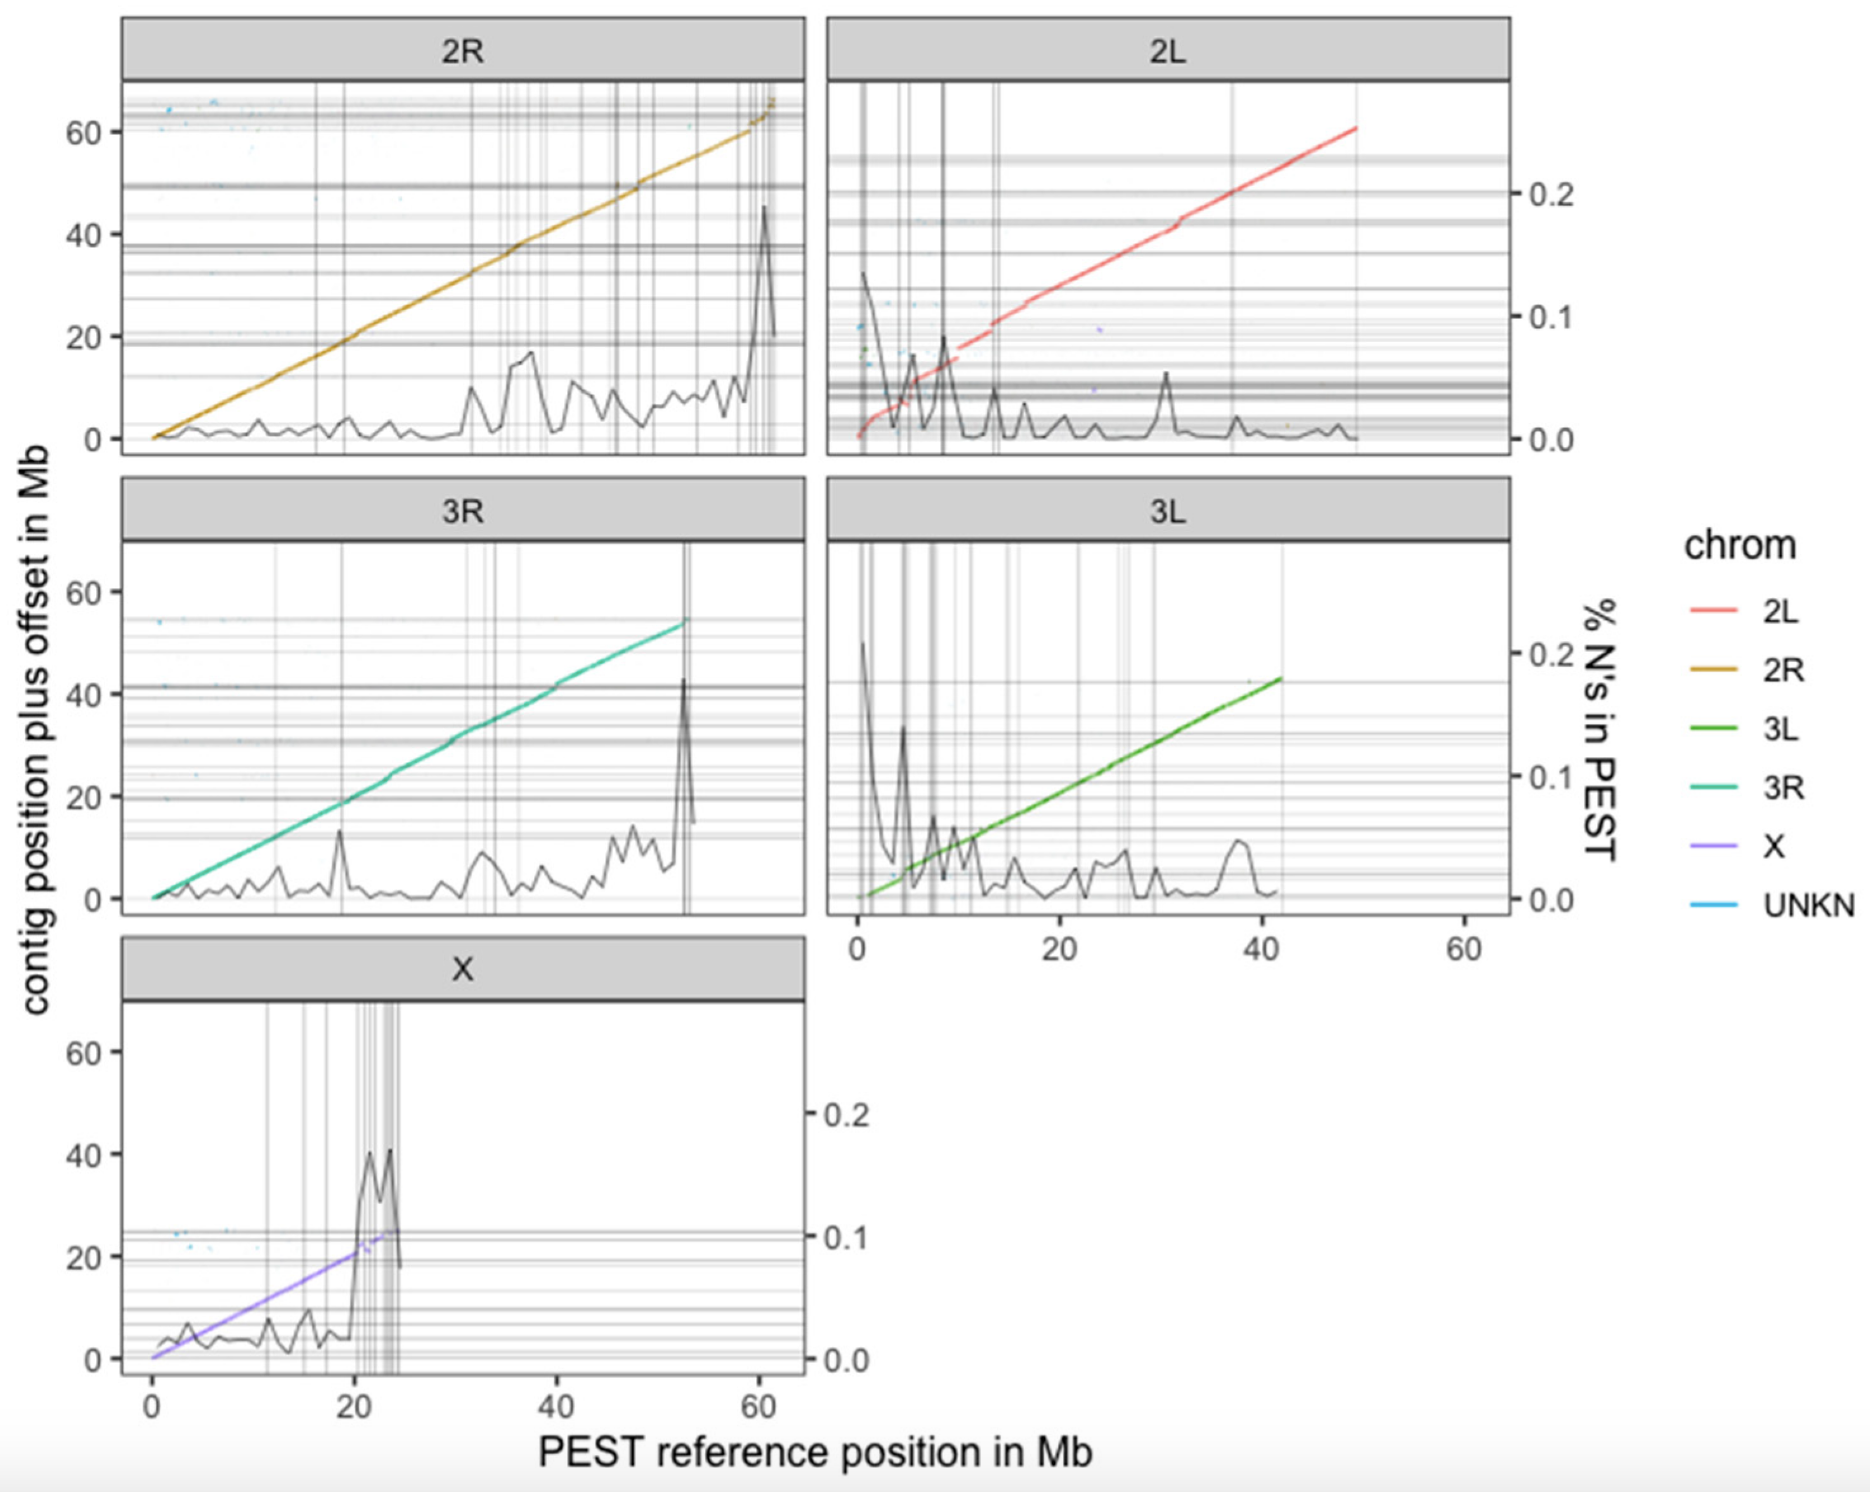
\includegraphics[width=1.0\textwidth]{dotplot.png}
\par{Alignment of the curated PacBio contigs to the AgamP4 PEST reference. Alignments are colored by the primary PEST reference chromosome to which they align but are placed in the panel and Y offset to which the contig as a whole aligns best. Contig ends are denoted by horizontal lines in the assembly and vertical lines in PEST. However, there are many Ns in PEST not annotated as contig breaks so the percent Ns per megabase of PEST is overlaid (scale on the right Y axis). There are no Ns in the PacBio assembly, but there may be gaps between the PacBio assembly contigs.}
\end{centering}
\end{figure}


\subsection{Identification and correction of misassembly}

\par{
Large regions (>200 kb) of discordant alignment of the contigs to the PEST reference where inspected further. Discordant alignments were categorized into one of three cases. 1. Large portions of a single contig aligned discordantly (e.g., to multiple PEST reference chromosomes). 2. Large regions in PEST where multiple assembly contigs aligned to the same reference region.  3. Large region in PEST where assembly contigs did not align. 
} \\
\par{
First, we considered discordant alignments where large portions of a single contig aligned in very different locations of the PEST reference. Using the alignment plots as described above, we colored each alignment by that contig's primary chromosome. Immediately one cross-chromosome contig alignment stuck out (see figure \ref{figure:misassembly}). We then evaluated the evidence for the assembly join at this breakpoint by aligning the subreads to the assembly and inspected the breakpoint region in IGV (figure \ref{figure:misassembly}). We found a repeat sequence that reads from each end would align into, but found no reads that spanned the repeat. This indicated to us that this was a chimeric misassembly, and we split the contig into two.
} \\
\par{
We also noted many smaller cross-chromosome alignments between contigs which primarily aligned to one of the five of PEST's chromosom-arm scaffolds and the UNKN (unknown) scaffold (not a true scaffold, just a collection of unplaced contigs). We discuss this further in section \ref{sectiong:unkn} by using these alignments to place genes and other genomic sequence in its proper chromosomal context which were previously unplaced.
}

\begin{figure}[htbp!]
\caption{Chimeric assembly}
\label{figure:misassembly}
\begin{centering}
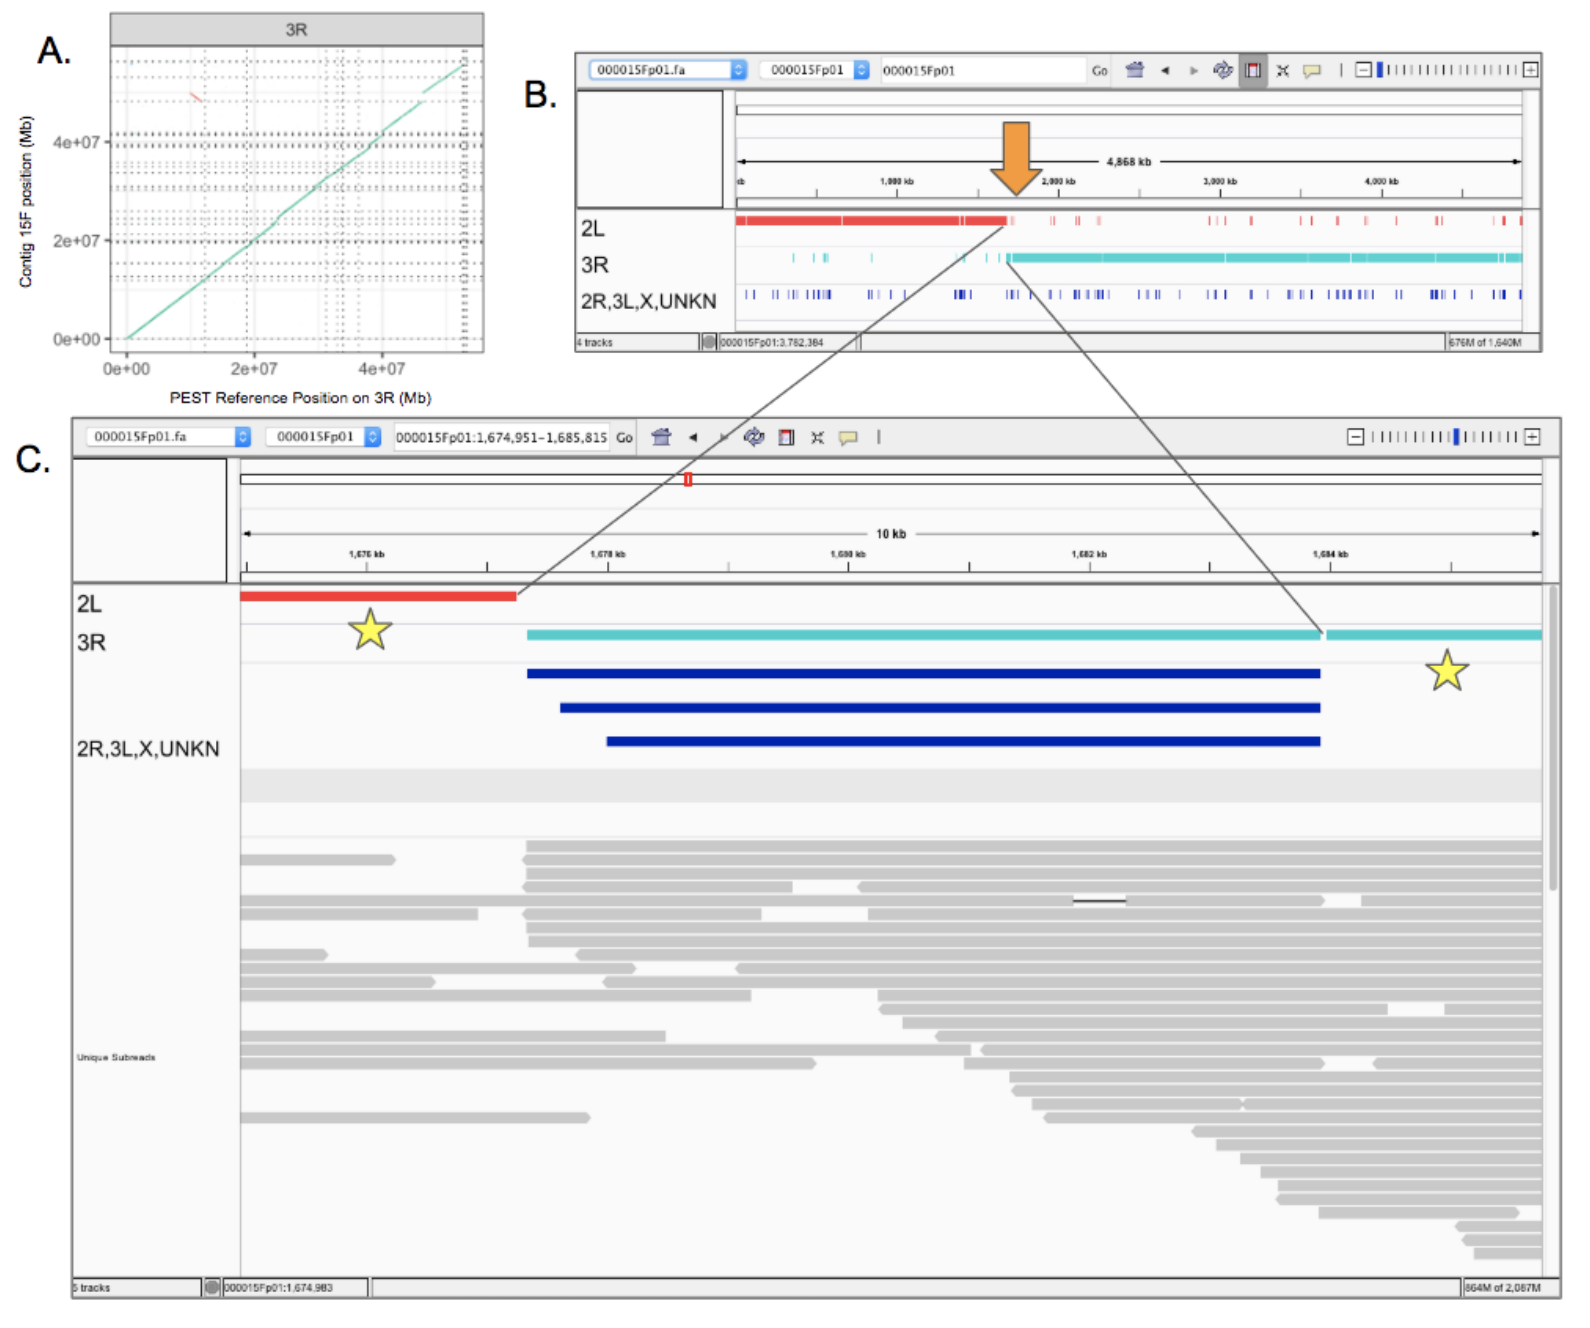
\includegraphics[width=1.0\textwidth]{misassembly.png}
\par{A chimeric contig between 2L and 3R. A. Alignment of PacBio contigs to PEST identifies a candidate chromosomal rearrangement. B. IGV screenshot of breakpoint (orange arrow) localized by alignment of contig to PEST. Red: alignment to 2L, turquoise: alignments to 3R, navy blue: alignments to other chromosomes and unplaced contigs. C. IGV visualization of mapped unique subreads at breakpoint shows 0 subreads mapping across the central repetitive region into the unique flanking sequence on the left (2L) and right (3R) (stars). A count of spanning reads was also determined with bedtools bamtobed utility. The 6.5kb central region aligns to four loci in the PEST genome and has ~370 bp of sequence similarity to the Tc1-like transposase gene in \textit{Anopheles gambiae}.}
\end{centering}
\end{figure}

\subsection{Remaining haplotig sequence on ends of contigs}

\par{
Next, large discordant regions where multiple contigs align to the same region in PEST were identified and evaluated. We find these regions by running samtools depth on the contig-PEST alignments, compressing to a bed file of contiguous regions of the same coverage, and then plotting to visually see where large sections are discordant (see figure \ref{figure:haplotig}). Using this, we found several very large segments of coverage two. Further inspection was done by zooming in to those regions specifically in the alignment plots. We observed that ends of contigs were aligned to the same position in the PEST genome. We then mapped the subreads to the assembly and assessed coverage in these regions. As expected if these were haplotig regions, the coverage was roughly half in the overlapping alignment regions. This clearly revealed that contigs were assembling the two haplotypes separately and were not removed by purge haplotigs. This is because purge haplotigs looks for contigs which are fully contained by another contig and it keeps the longer contig and removes the shorter haplotig. This results in regions where the assembly has assembled both haplotypes separately but one contig does not fully contain the other contig, the haplotig sequence remains (see figure \ref{figure:haplotig}). This realization spawned another project in our lab to improve haplotig purging by combining coverage of reads mapped to the assembly with sequence similarity to identify and remove haplotig sequence even when not fully contained by another contig\cite{purgedups} improving on the two previously available methods\cite{purge}\cite{haplomerger}.
}


\begin{figure}[htbp!]

\caption{Evidence of remaining haplotig contig ends.}

\label{figure:haplotig}
\begin{centering}
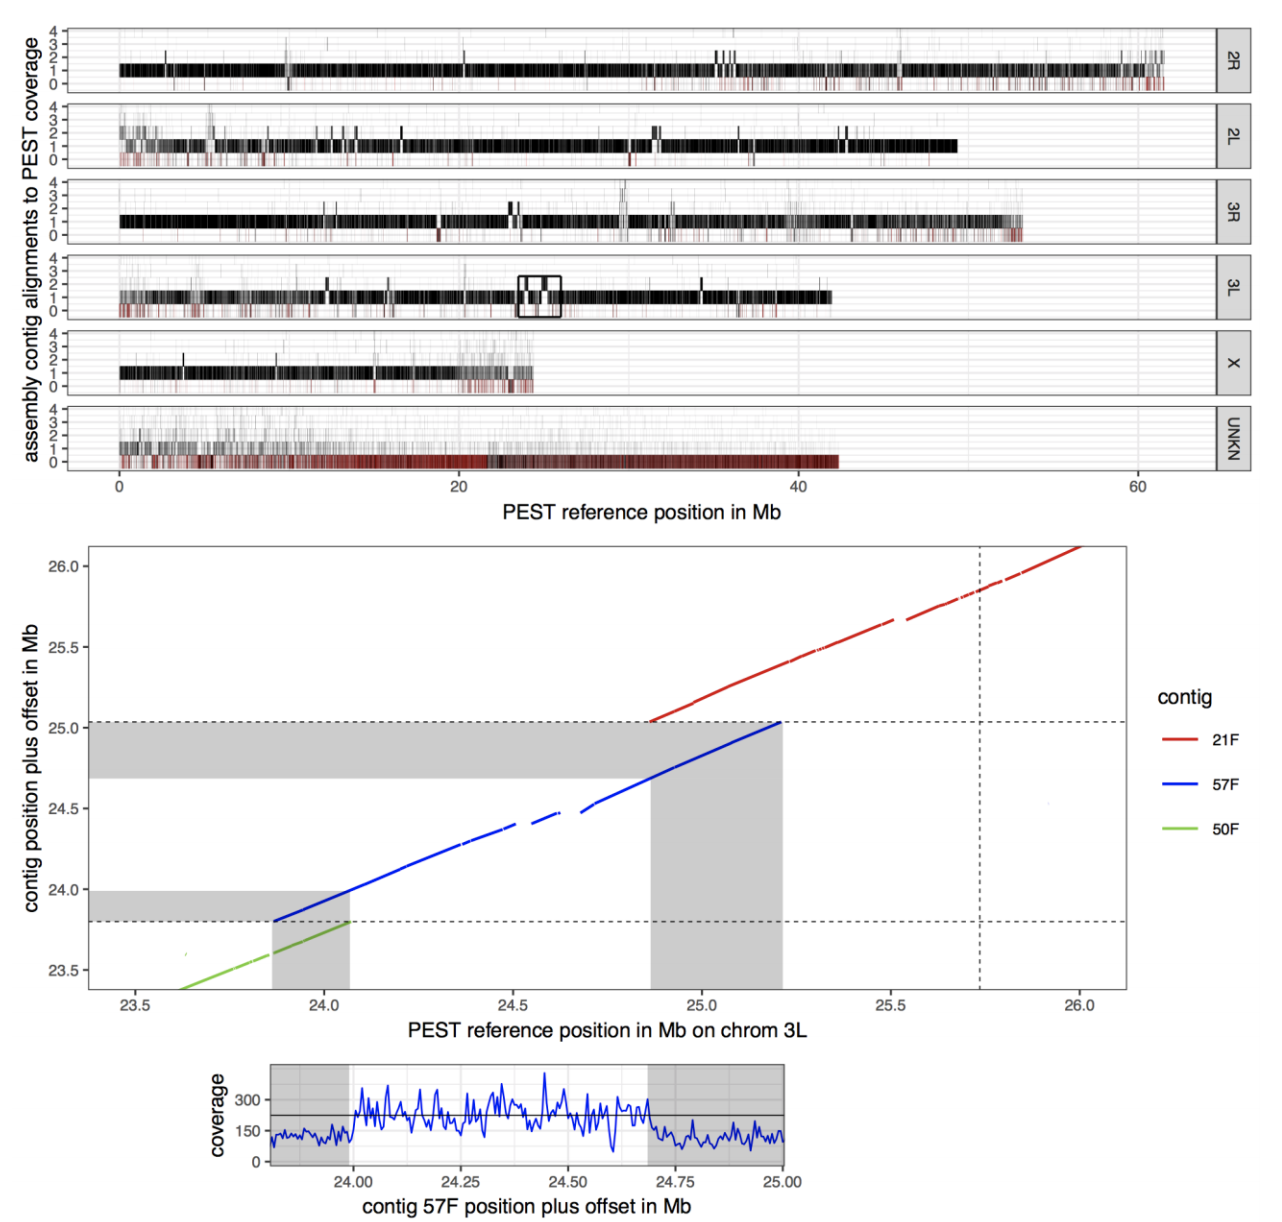
\includegraphics[width=\textwidth]{haplotigity.png}
\par{Alignment and coverage plot (top) of the PacBio assembly contigs relative to PEST,
and magnification of one area of excess coverage (bottom). In the top panel, the number of
alignments of PacBio contigs to PEST are represented by black bars, with most of the genome
showing a 1:1 correspondence to PEST. Red denotes Ns in the reference. Isolated areas of
higher number of contig alignments are visible, one of which (black box) is magnified in the
bottom panel. Here, the ends of neighboring contigs overlap, which is currently not resolved with
the Purge Haplotigs software since the overlap is only partial. The sequencing depth of PacBio
reads for the central (blue) contig (57F) corroborate this interpretation, exhibiting half of the
expected coverage in the greyed regions of contig overlap, and with the corresponding ends of
the red and green contigs complementing with the other half of coverage, respectively (not
shown for clarity).}
\end{centering}
\end{figure}

\par{
And finally, we consider large discordant regions in which no assembly contigs align to the PEST reference. In general this is rare in the chromosomal scaffolds. Most of the zero contig-coverage areas of the contig on PEST alignment file are location in which the PEST contains Ns. And the large majority of zero contig coverage areas are in the UNKN scaffold. We explored the largest of the zero contig coverage region in the chromosomal PEST scaffolds (figure \ref{figure:nocovplot}). We see that this region is flanked by sections of Ns and that very few PacBio subreads map to the non N regions between indicating that this sequence may be low quality, possible derived from contamination, or be a biological difference (large insertion in PEST) between the two species.
}

\begin{figure}[htbp!]

\caption{No contig coverage region}
\label{figure:nocovplot}
\begin{centering}
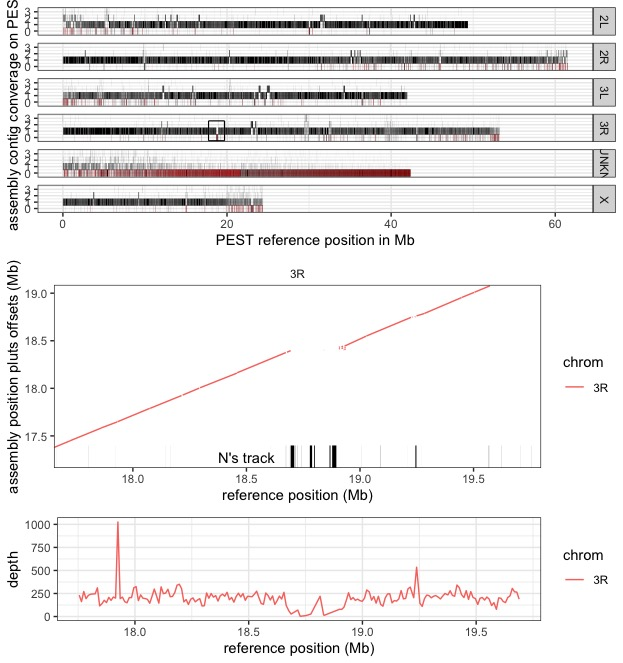
\includegraphics[width=1.0\textwidth]{Nocovplot.jpeg}
\par{ Top: outlines large region with zero coverage in chromosomal scaffold 3R on PEST reference. Middle: Zoom in of alignment plot in that region with Ns track showing regions of Ns flanking this sequence with another section of Ns in the middle. Bottom: shows subread depth when aligned to the PEST reference showing decreased mapping in this region.}
\end{centering}
\end{figure}



\subsection{Expansion of previously collapsed repeat}

\par{
The new PacBio assembly makes many improvements when compared to the PEST assembly. For example, a single contig from the new PacBio assembly expanded a tandem repeat region on chromosome 2L that in PEST was collapsed, while also filling in many Ns (gaps) in PEST, and also spanning a break between PEST scaffolds set to 10,000 Ns (see figure \ref{figure:repeat}).
}

\begin{figure}[htbp!]

\caption{Example of expansion of previously collapsed repeat}
\label{figure:repeat}
\begin{centering}
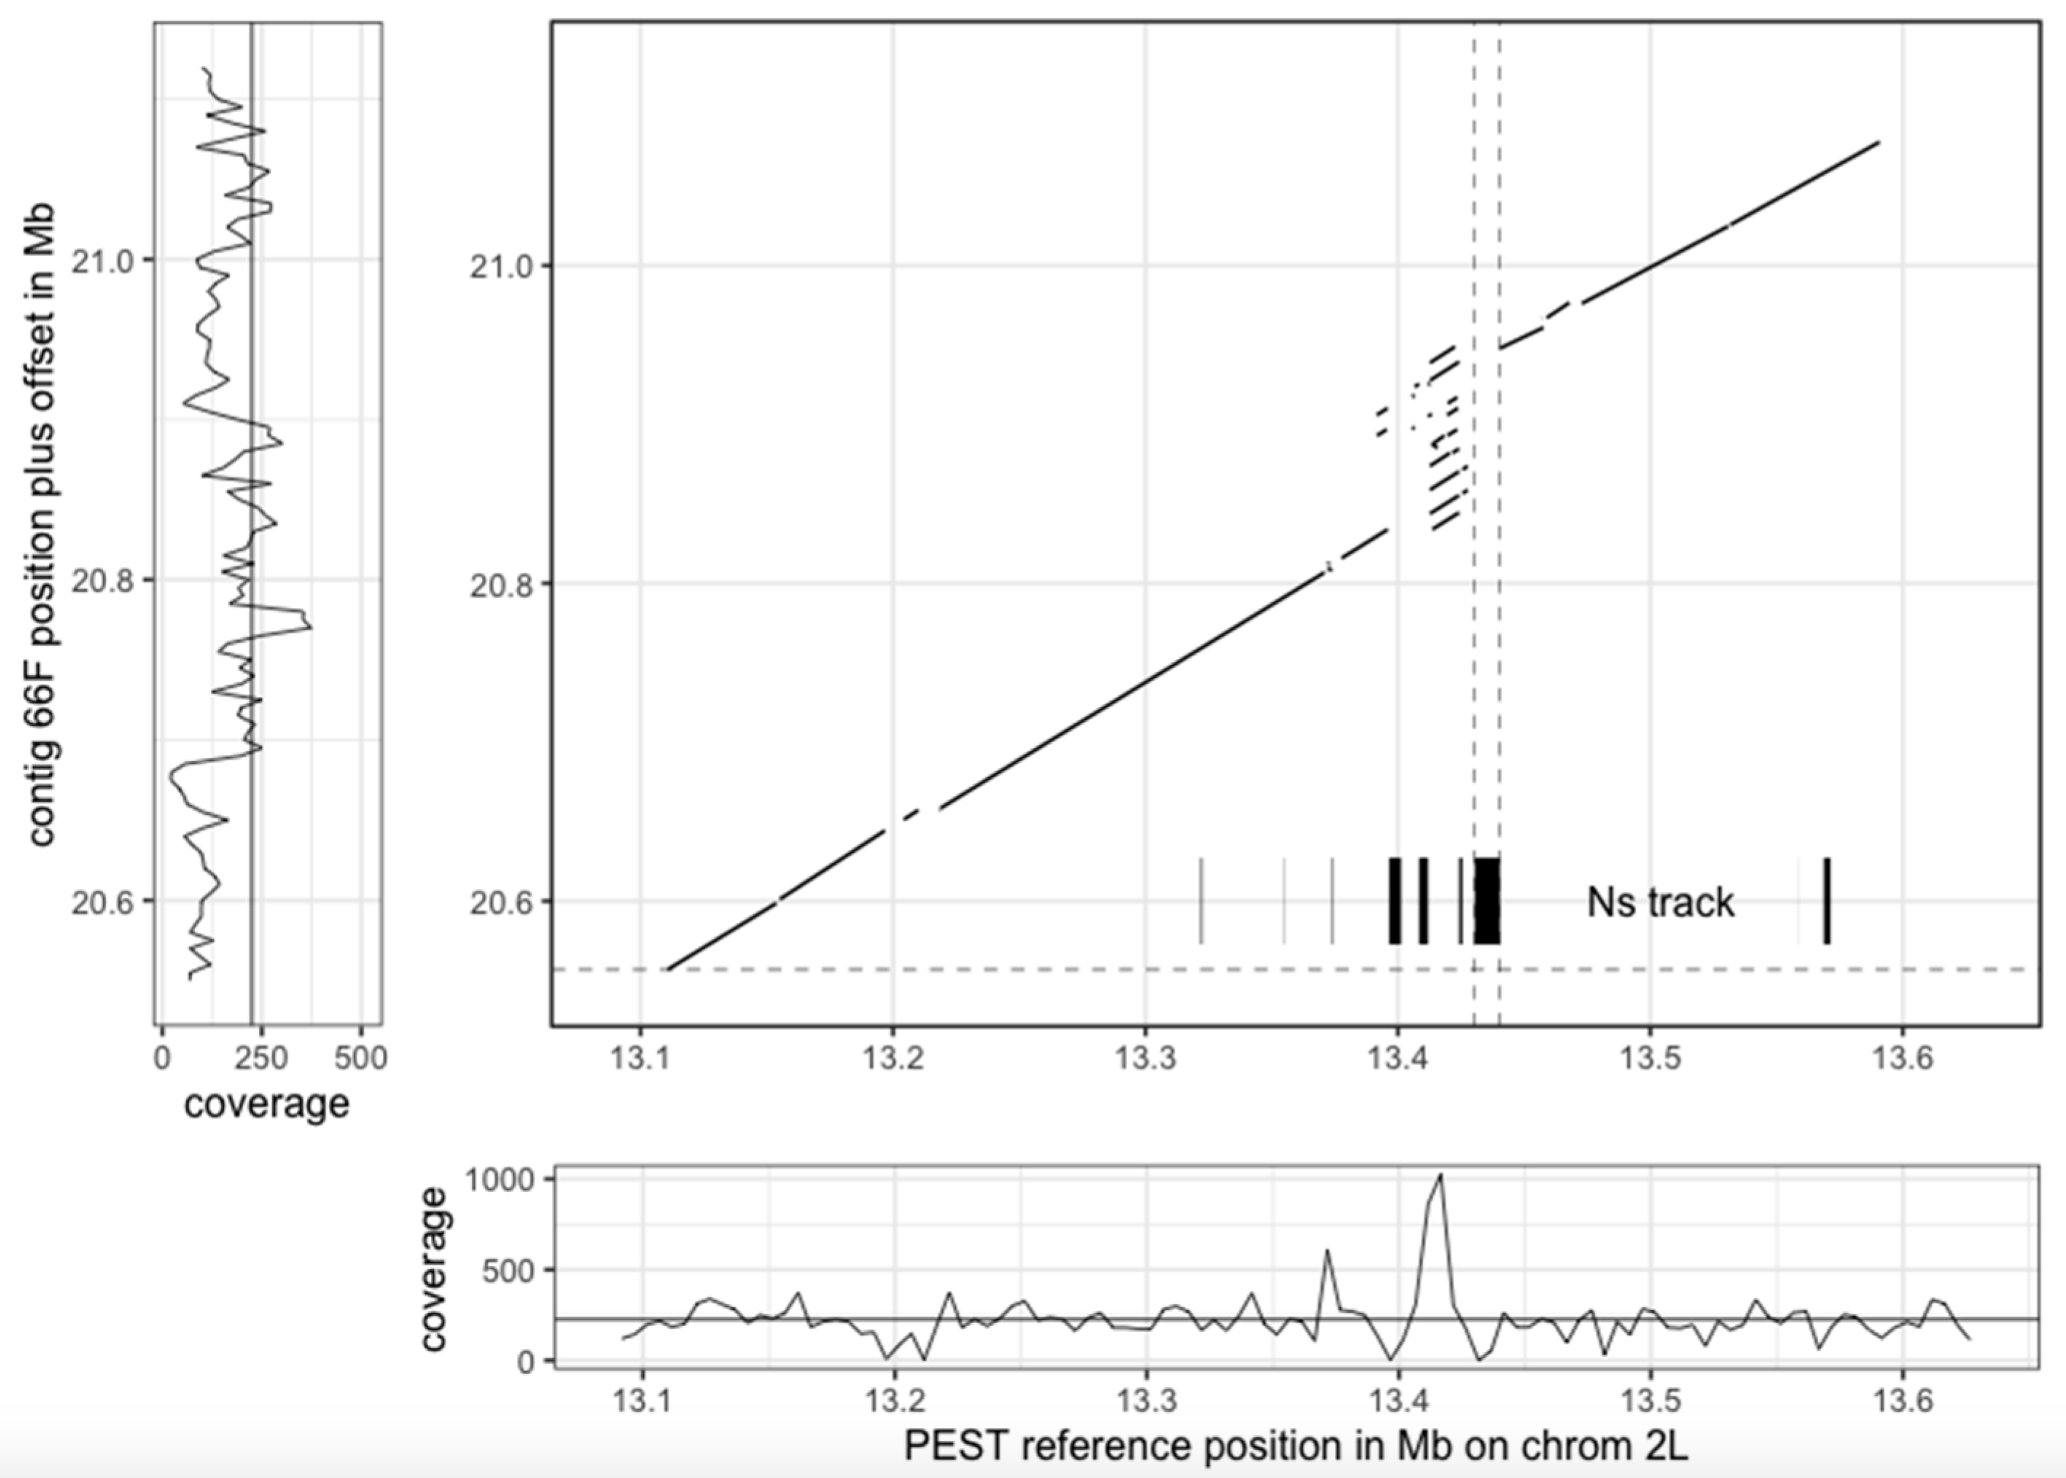
\includegraphics[width=1.0\textwidth]{repeatexpansion.png}
\par{ Example of a compressed repeat in PEST that has been expanded by the PacBio assembly. Dotted vertical lines represent a gap in the PEST assembly (10,000 Ns) between scaffolds, which is now spanned by the single PacBio contig. Coverage plot of the PacBio subreads aligned to PEST (bottom) highlights the region where excess coverage indicates a collapsed repeat in PEST, in contrast the coverage of PacBio subreads aligned to the PacBio contig (left) is more uniform. }
\end{centering}
\end{figure}

\subsection{Corrected order and orientation vs PEST scaffolding}

\par{
We also identified several potential rearrangements in the 20-22 Mb region of the X chromosome (see figure \ref{figure:x_inversion}). PEST has contig breaks at the putative breakpoints relative to the assembly, however, given that a single PacBio contig spans the full region and that potential breakpoints relative to PEST are supported by multiple reads, the most likely explanation is an order and orientation issue in PEST, perhaps combined with a potential inversion difference between \textit{Anopheles coluzzii} and the PEST reference. In addition, the contig contains a relatively large region (~380 kb in total) of PacBio sequence corresponding to several pieces in the UNKN section of PEST that can now be assigned to the X chromosome.
}

\begin{figure}[htbp!]

\caption{Resolved order and orientation error in PEST scaffolding}
\label{figure:x_inversion}
\begin{centering}
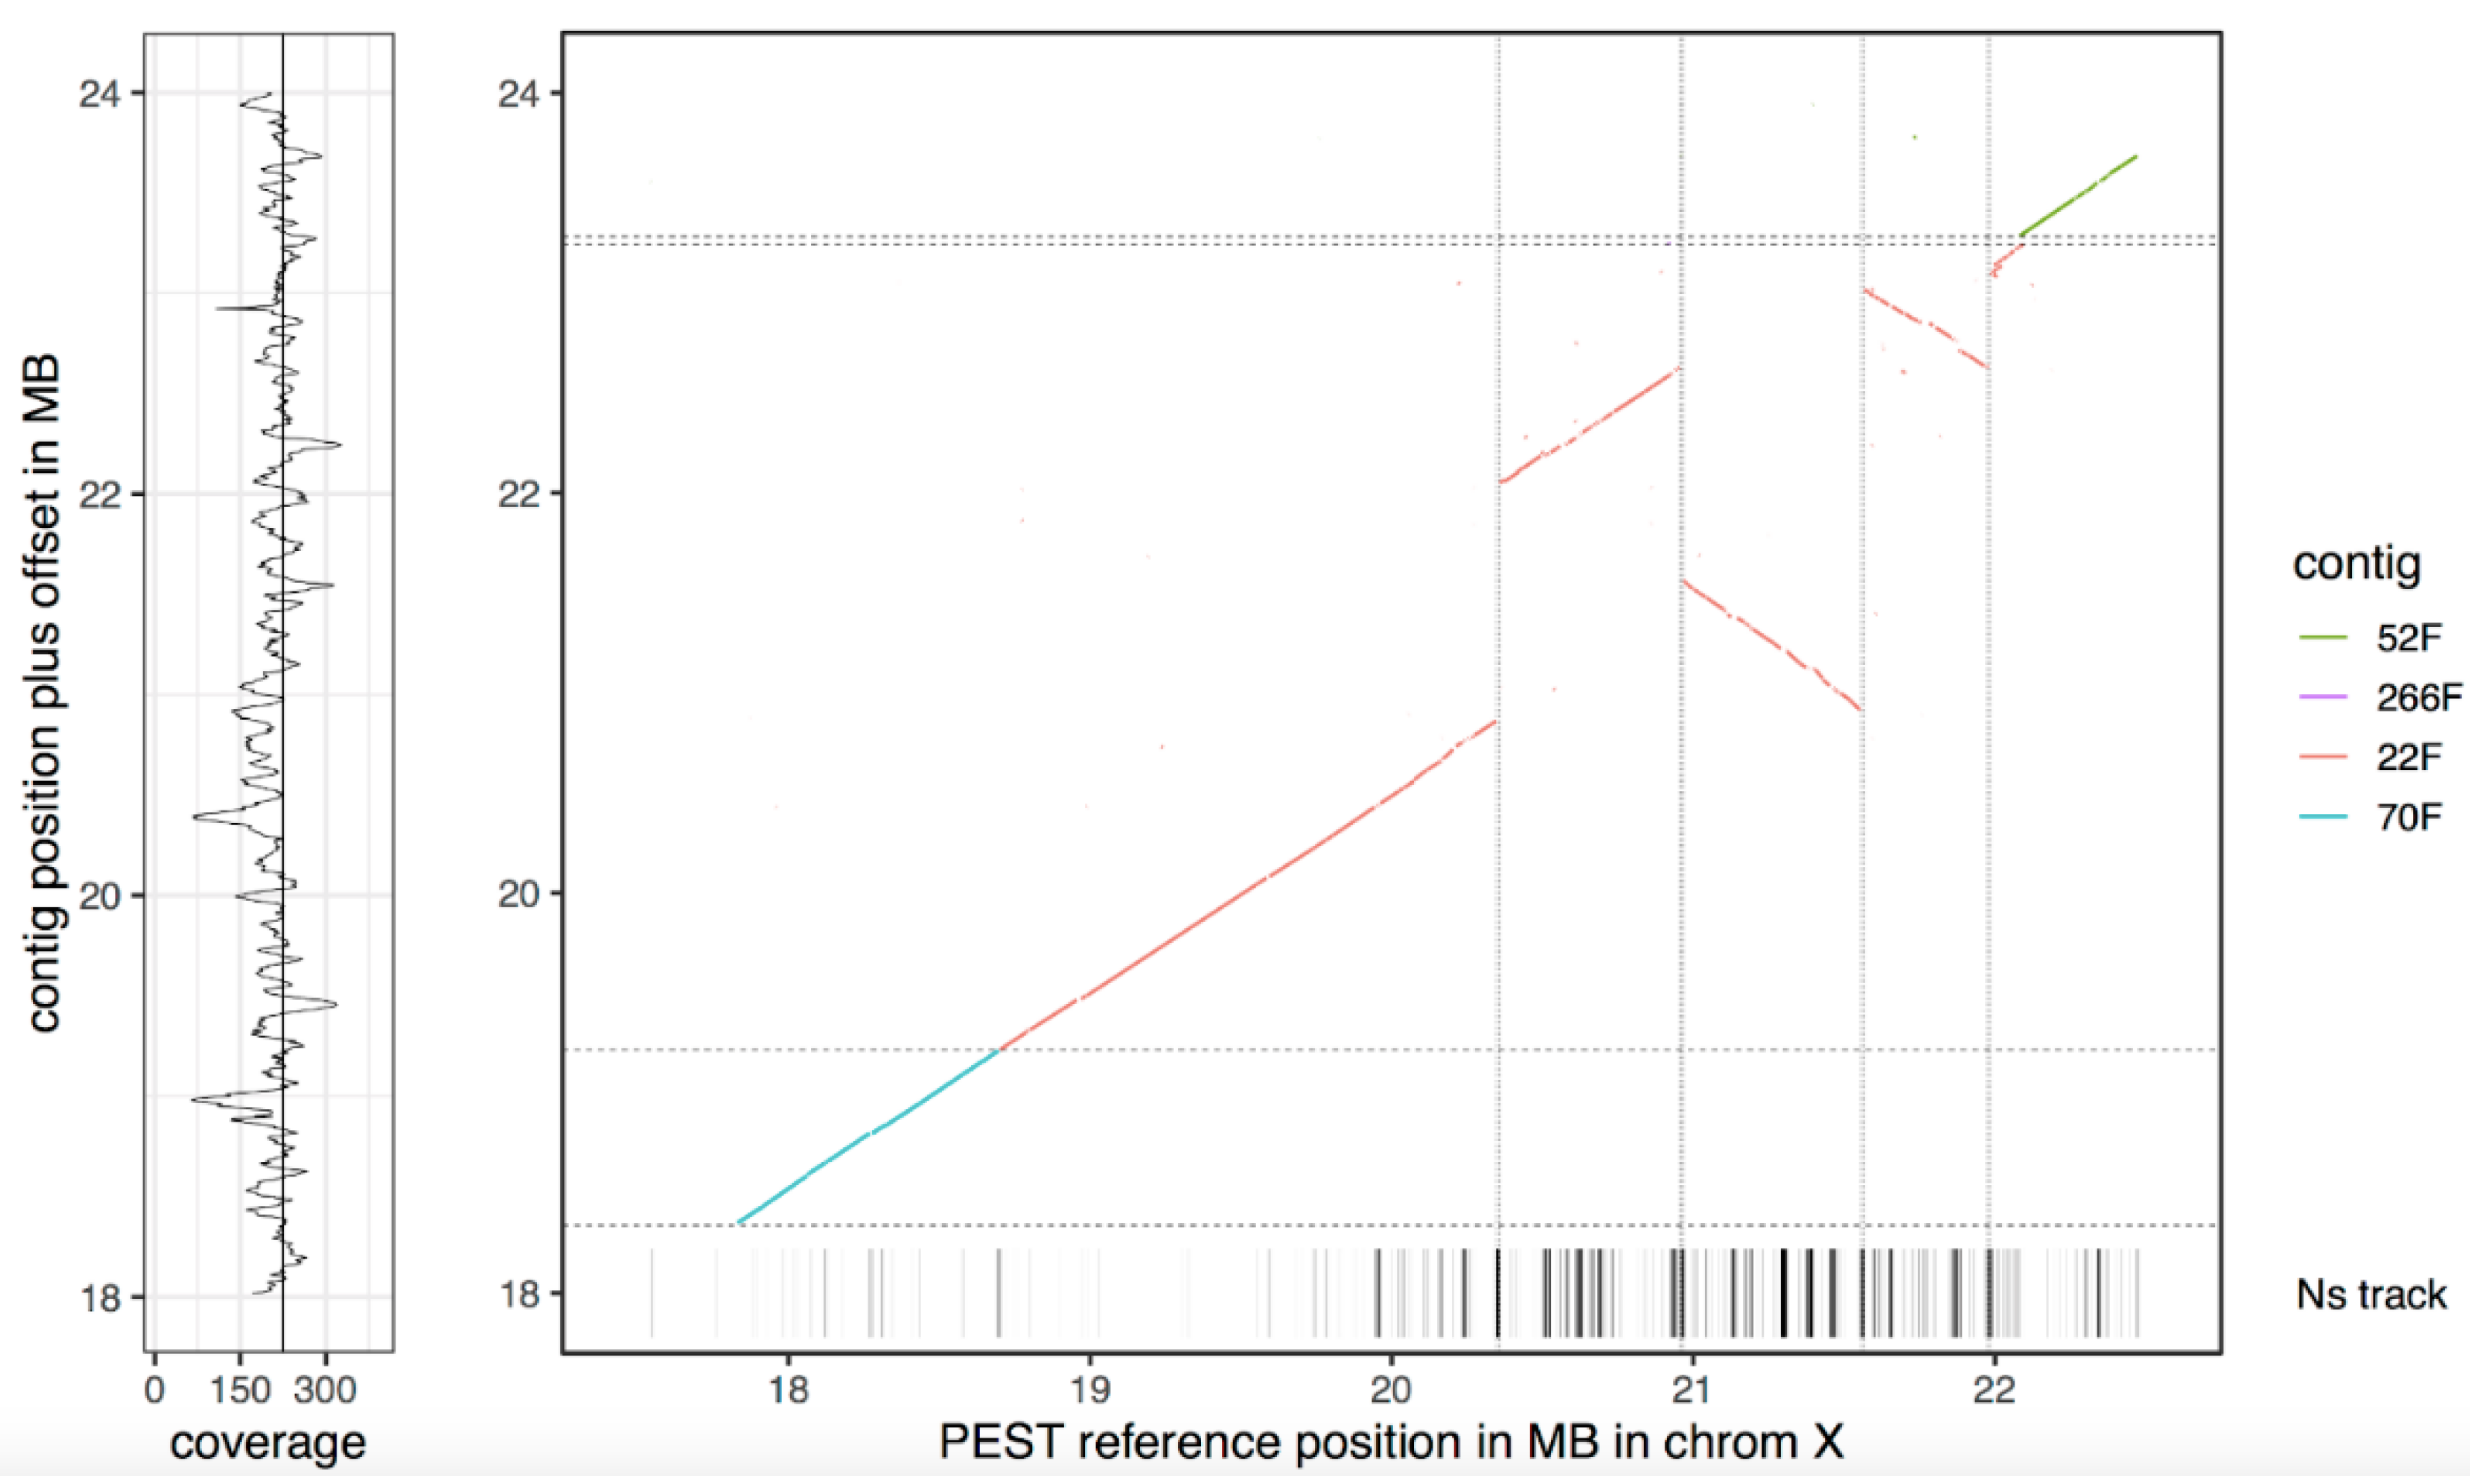
\includegraphics[width=1.0\textwidth]{x_inversion.png}
\par{Alignment of X pericentromeric contigs to PEST, highlighting likely order and orientation issues in the PEST assembly that are resolved by a single PacBio contig.}
\end{centering}
\end{figure}


\subsection{Identification of some UNKN PEST sequence as haplotigs}

\par{
The PEST annotation also retains a large bin of unplaced contigs (27.3 Mb excluding Ns) designated as the UNKN (unknown) chromosome. Previously, we mapped either assembly contigs onto the PEST reference or subreads against the assembly. Now we do the reverse of the former and map PEST contigs onto the assembly. If an UNKN contig alignment overlaps a chromosomal contig alignment versus the assembly (both with mapping quality (mapq) 60), it is likely to be a haplotig in the UNKN (see figure \ref{figure:unknplace}). In total, we find that 7.27 Mb are haplotigs (i.e., also have high quality PEST chromosomal alignments to the same location in the assembly).
}

\begin{figure}[htbp!]

\caption{UNKN placement and haplotig identification}
\label{figure:unknplace}
\begin{centering}
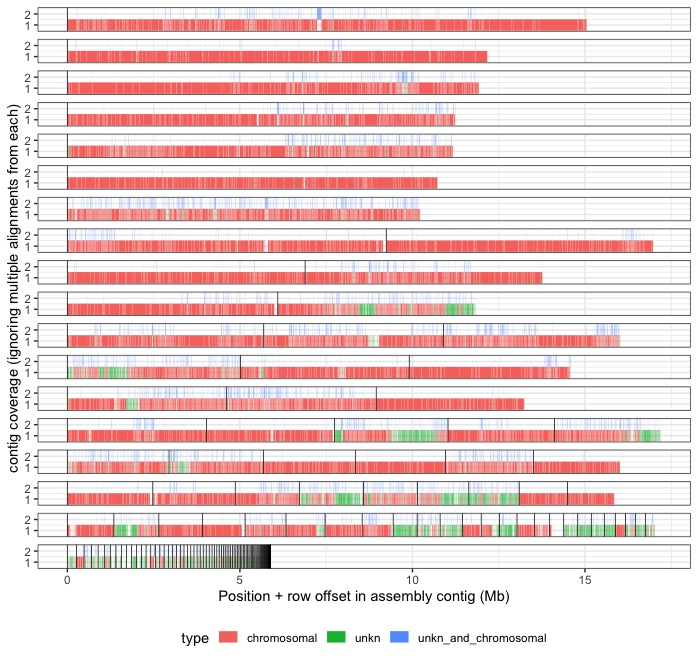
\includegraphics[width=1.0\textwidth]{Unkn_placement_haplotig.jpeg}
\par{Contig coverages (ignoring multiple alignments for each chromosomal and UNKN sequence) of PEST aligned to the curated assembly showing placement of previously unplaced sequence (green on contigs that also have red (chromosomal) alignments). We also note the locations where both UNKN and chromosomal sequence align to the same location in the curated assembly which are likely haplotigs in the PEST UNKN scaffold.}
\end{centering}
\end{figure}

\subsection{Placement of previously unplaced genes}\label{section:unkn}
\par{
In addition to the UNKN haplotig sequences, we found another 10.9 Mb of the alignments are newly placed sequence that do not overlap with PEST chromosomal alignments but are in contigs which have a large amount (>100kb) of chromosomal alignments meaning these contigs are confidently ordered and oriented in their chromosomal contexts. The UNKN bin also contains 737 annotated genes. Remarkably, our single-insect assembly now places 667 (>90\%) of these formerly unplaced genes into their appropriate chromosomal contexts (2L:148 genes; 2R:162 genes; 3L: 126 genes; 3R:91 genes; X:140 genes; unplaced:70 genes; detail on placement of specific genes can be found in the supplement of our paper \cite{singlemosquito}), which together with their flanking sequence comprise 8.9 Mb of sequence. Altogether, this means that 32.6\% of the UNKN chromosome is now placed in the genome and 26.6\% is determined to be haplotigs, along with 90\% of the genes that were contained within it. Much of the remaining sequence do not have high mapping quality subreads when aligning subreads to the PEST reference meaning they are either repeats or junk sequence.
}

\begin{table}[htbp!]
\caption{Placement of previously unplaced genes}
\label{table:unplaced}
\begin{tabular}{ | l | l |}
\hline
 Chromosome arm & Number of placed genes  \\
 
 \hline
 2L & 148 \\
 \hline
 2R & 162 \\
 \hline
 3L & 126 \\
 \hline
 3R & 91 \\
 \hline
 X & 140 \\
 \hline
 unplaced & 70 \\
 \hline
\end{tabular} 
\end{table}

\subsection{PEST contig coverage on PacBio curated assembly}

\par{
In addition to looking for the two contig coverage areas and confirming that they primarily come from haplotigs in the UNKN scaffold, we would like to inspect for other abnormalities such as zero contig coverage regions. In figure \ref{figure:reverse_coverage} we see some significant zero coverage regions. However, most of these are intermittently zero and one likely just indicating sequence divergence rather than an incomplete PEST reference. There are a few more solidly zero coverage regions, but they are not dramatically long (<200Kb). Still, we know from the BUSCO \ref{table:busco} analysis that there are fewer complete genes and more fragmented and missing genes in the PEST reference as compared to the PacBio assembly. These regions likely account for some of that difference.
}

\begin{figure}[htbp!]

\caption{PEST contig coverage when aligned to PacBio curated assembly}
\label{figure:reverse_coverage}
\begin{centering}
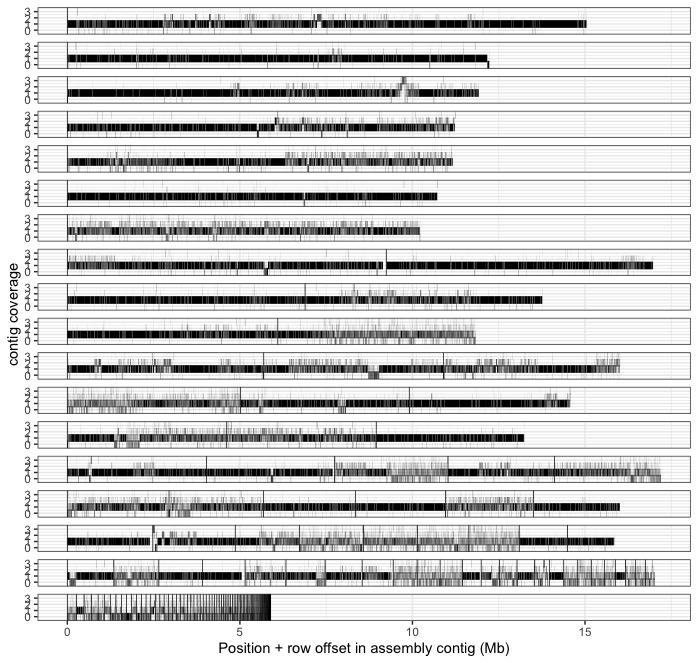
\includegraphics[width=1.0\textwidth]{Reverse_contig_coverage.jpeg}
\par{Contig coverages of PEST aligned to the curated assembly. When comparing to figure \ref{figure:unknplace} we see that most of the two coverage likely come from haplotigs in the UNKN scaffold. But we do see some significant zero coverage areas as well.}
\end{centering}
\end{figure}

\section{Discussion}

\par{
Long-read PacBio sequencing has been utilized extensively to generate high-quality eukaryote de novo genome assemblies, but because of the relatively large DNA input requirements, it has not been used to its full potential for small organisms, requiring time-consuming inbreeding or pooling strategies to generate enough DNA for library preparation and sequencing. Here we present, to our knowledge, the first example of a high-quality de novo assembly from a single insect. This assembly, using only one individual and one sequencing technology, exhibits a higher level of contiguity, completeness, accuracy, and degree of haplotype separation than any previous Anopheles assembly, demonstrating the impact of long reads on assembly statistics. While the assembly did not achieve independent full chromosomal scale assignment of contigs, its mega-base scale contiguity without gaps immediately provides insights into gene structure and larger-scale genomic architecture, such as promoters, enhancers, repeat elements, large-scale structural variation relative to other species, resolution of tandem repeats (figure \ref{figure:x_inversion}), and many other aspects relative to functional and comparative genomics questions.
} \\
\par{
About a third of the genome for this diploid individual is haplotype-resolved and represented as two separate sequences for the two alleles, thereby providing additional information about the extent and structure of heterozygosity that was not available in previous assemblies, which have been constructed from many pooled individuals. In contrast with approaches requiring multiple individuals, the ability to generate high-quality genomes from single individuals greatly simplifies the assembly process and interpretation, and will allow far clearer lineage and evolutionary conclusions from the sequencing of members of different populations and species. Further, if parental samples are available, the recently developed trio binning assembly approach \cite{triobinning} can be used to further segregate alleles for a full haplotype-resolved assembly of both parental copies of the diploid offspring organism.
} \\
\par{
The assembly presented here provides an excellent foundation towards generating an improved chromosome-scale reference genome, using the previous PEST reference, scaffolding information from genetic maps, technologies such as Hi-C (e.g., \cite{falconphase}), or alignment of the contigs to closely related species' references. These approaches can also be used to highlight areas of potential improvements to the FALCON-Unzip assembler and to Purge Haplotigs, or other packages used to identify haplotypic contigs. As one example, we noticed in the context of the incomplete haplotype purging described above that some neighboring contig ends exhibited overlaps relative to the PEST reference (figure \ref{figure:haplotig}). The interpretation of such haplotype contig overlaps was corroborated by the observed halving of average sequencing depth over the regions of overlap. These methods could incorporate adjustments to try to account for haplotypic regions in the ends of contigs rather than complete contigs being fully haplotypic.
} \\

\par{
We noted the importance of the initial DNA size distribution in conjunction with this protocol. Since neither shearing prior to library construction nor size-selection thereafter were employed, the starting high-molecular weight DNA should contain fragments at greater than ~20 kb on average, and without the significant presence of short (smaller than ~5 kb) DNA fragments. Further research into suitable DNA extraction, storage and transportation methodologies is needed to fulfill these requirements for a broader spectrum of different species and environments, in order to allow for the preparation of suitable DNA samples from wild-caught samples originating in sometimes remote areas with limited sample preparation infrastructure.
} \\
\par{
We anticipate that the new workflow described here will facilitate the sequencing and high-quality assembly of many more species of small organisms, as well as groups of individuals within a species for population-scale analyses, representing an important prerequisite in view of large-scale initiatives such as i5K and the Earth BioGenome Project \cite{EBGP}\cite{arthropoddiversity}. In addition, other research areas with typically low DNA input regimes could benefit from the described new workflow, e.g., metagenomic community characterizations of small biofilms, DNA isolated from needle biopsy samples, minimization of amplification cycles for targeted or single-cell sequencing applications, and others.
}



%!TEX root = ../thesis.tex
%\input{commands.tex}
%*******************************************************************************
%****************************** Third Chapter **********************************
%*******************************************************************************
\chapter{Haplotype phasing consistency as a signal for physical linkage in scaffolding and assembly}

% **************************** Define Graphics Path **************************
\ifpdf
    \graphicspath{{Chapter4/Figs/Raster/}{Chapter4/Figs/PDF/}{Chapter4/Figs/}}
\else
    \graphicspath{{Chapter4/Figs/Vector/}{Chapter4/Figs/}}
\fi



\section{Background}
\par{
Reference genomes have enabled a range of genomic analysis by providing prior knowledge of the sequence 
and giving genomic context as well as a common coordinate system by which to compare multiple genomes \cite{1000genomes} \cite{GRCh38}. Assembling reference genomes is complicated by repetitive sequences, heterozygosity, and sequencing errors. As discussed in Chapter 3, when an assembly encounters inexact homologous sequences, it must determine which of these cases the sequence differences are due to. 
If the assembler cannot distinguish between heterozygosity and repeats, and if no reads span the homologous sequence into more unique regions, the contig must end
to avoid assembly distant regions or sequence from different chromosomes together. Historically reference genomes were created by large haploid bacterial artificial chromosomes (BACs) clone libraries \cite{human}. 
These methods overcame much of the problem of resolving repeats and heterozygosity because of their length allowing them to read through all but the longest segmental duplications and the fact that they are inherently haploid. However, because each of these BACs were sequenced with Sanger sequencing and assembled, they were still subject to problems in repeats longer than the Sanger reads that were close enough to one another to occur in the same BAC clone. But most importantly, these methods are far too costly to apply to many genomes. 
}

\par{
More recently the cost reductions of long read technologies \cite{pacbio} \cite{oxford}, and reduced error profiles through optimization of the circular consensus method \cite{ccs}\cite{HIFI}
as well as the emergence of other long range genetic information technologies \cite{10xlinked} \cite{HiC} \cite{bionano} 
have converged to make high quality, cost effective reference genomes. This has then resparked interest in assembly 
as well as large reference generation projects. Efforts have begun on the Earth Biogenome Project (EBP)\cite{EBGP}, a global project to sequence the entire diversity of multicellular eukaryotic life. In the UK, the Sanger Institute and partners have started to sequence 60,000 species from the British Isles in the Darwin Tree of Life (DToL) project. These projects aim to provide a scientific resource for the next generation of biological science, for environmental conservation, and to study evolution at a much broader and deeper scale than ever before. 
}

\par{
As discussed in Chapter 3, one of the primary remaining difficulties in assembling reference quality genomes is high levels of heterozygosity such as found in many of the non-model organisms included in the EBG and DToL projects. While Chapter 3 focused on going from a pool of individuals---and thus many haplotypes---to a single individual---and thus two haplotypes, this chapter focuses on the problems encountered with high levels of heterozygosity within an individual and the improvements that can be made computationally to both alleviate those problems as well as use the high levels of heterozygosity to our advantage. 
For these newer technologies mentioned above, there are now assembly algorithms that deal with each data type \cite{falcon} \cite{supernova} \cite{bionano_assembly} 
as well as combinations of multiple technologies \cite{genemyers} \cite{hybrid10x} \cite{hicscafffirst}\cite{hicassembly}. 
 These methods try to co-assemble both haplotypes arriving at a haploid consensus \cite{watchtower} \cite{canu} 
 or a diploid assembly \cite{falconPHASE} \cite{supernova} \cite{hifiasm}\cite{dipasm}, but heterozygosity still injects complexity and ambiguity on top of a haploid assembly process.
}

\par{
As mentioned in Chapter 3, one method for dealing with the problem of heterozygosity is inbreeding organisms to a point of low heterozygosity \cite{drosophila}, 
but this is not possible for all organisms. Trio-sga used pedigree sequencing information in the assembly algorithm \cite{trio-sga} 
but was built for short reads and does not work on long read data. Recently Koren et al. described trio binning which uses a mother-father-child trio to 
separate long reads into their haplotype of origin prior to haploid assembly \cite{triobinning}. 
While this method is very effective, creating such a cross would be infeasible for many species and costly for the vast number of reference genomes these projects intend to sequence. 
Another recent approach using the new highly accurate HIgh FIdelity (HIFI) ccs reads from PacBio along with homopolymer compression and other methods to reduce errors dramatically is to 
require nearly identical sequence similarity to extend the assembly graph \cite{HICANU}. This results in the haplotypes being b v separately in all but the few long stretches of homozygosity in 
a genome. They then run a haplotic purging software PurgeDups \cite{purgedups} to remove one of the haplotype assemblies. This has the downside of not matching the haplotypes to make comparisons, but that could be done 
fairly well as an additional analysis step. This method does not explicitly phase the haplotypes and may have long phase switches especially across long regions of homozygosity.
}

\par{
Despite the incredible advances made over the past several years in both sequencing technologies and assembly methods, we still cannot assemble whole chromosomes or chromosome arms with a 
single technology for most organisms. After assembly we are left with some level of fragmentation of chromosomes into contiguous sequences (contigs) which we wish to scaffold together. While the 
PacBio HIFI technology has many wonderful properties including continuous, highly accurate reads, it does not produce long enough reads to span many repeat or low sequence complexity regions in most genomes.
 10x Genomics linked read technology, however, will create barcode linked short reads across much longer molecules (50kb+) with some molecules reaching well over 250kb \cite{10xlinked}. Optical map technology in which the DNA is linearized and flourescent markers are attached to sequence specific loci via restriction digestion and optically inspected can give sparse data for pieces of DNA about as long as can be isolated with modern high molecular weight extraction methods\cite{opticalmaps1}. And high-throughput chromatin conformation capture sequencing (Hi-C) data creates links between sequences physically located close to one another. And while there will be cross-chromosomal links, the large majority of links are intra-chromosomal but can create links of almost any length \cite{3CHIC} \cite{HIC}. Each of these technologies have been used to break misassemblies in contigs and scaffold contigs\cite{scaff10x}\cite{opticalhuman}\cite{hicscafffirst}\cite{SALSA}\cite{GRAAL}\cite{instaGRAAL}. But some of these scaffolders have been known to introduce misassemblies \cite{hicscafffirst}. 
}


\par{
While high levels of heterozygosity make the assembly problem harder for traditional methods, haplotype phasing consistency (reads containing multiple heterozygous alleles segregate into two---if diploid---groups according to which alleles they have) can be used as a signal of physical linkage in both assembly and scaffolding and as a method to differentiate inexact repeats from haplotype differences. While the conventional thinking is that heterozygosity makes these problems more difficult, we turn this around and use the phasing consistent property of heterozygous sites as a powerful way to simplify and add statistical power to them. In this chapter we present a toolkit for phasing, phasing aware assembly, and phasing aware scaffolding called phasstools (PHasing and ASSembly tools). It is made up of a number of github repositories with a master repository to give a unified command line interface. The code is open source and available at https://github.com/wheaton5/phasstools and the submodule repositories which are linked from the main repository. The use cases are reference based and fully de novo haplotype phasing, assembly based phasing aware scaffolding, and phasing aware assembly. While I will show results from the phasing aware assembly, these are preliminary and not without problems, which I will discuss. For that reason, I will first address the steps required to use phasing consistency for highly accurate assembly scaffolding. First I will outline phasing consistency, then introduce heterozygous single nucleotide polymorphism (SNP) kmer pairs as a mechanism for fully de novo haplotype phasing. Next I introduce an algorithm for de novo haplotype phasing using sparse \textit{Bernoulli} mixture model clustering---an algorithm very similar to the clustering algorithm used in Chapter 2. Afterwards I describe a phasing algorithm based on a given assembly to then be used for phasing aware scaffolding.
}


\section{Phasing aware scaffolding of an existing assembly: phasst scaff}

\par{
Our goal is to use the phasing consistency of Hi-C reads and optionally linked reads that cover heterozygous sequence on two contigs. First we must find those heterozygous sites. Then we can define phasing consistency of those sites.
}


\subsection{Paired heterozygous SNP kmers}
\par{
In the case of scaffolding an existing assembly, we could map the reads to the assembly and call variants to find heterozygous sites as is the common workflow for resequencing efforts. In an effort to be unbiased by the 
assembly, and to be general to a de novo assembly process, we will use paired SNP kmers---kmers that vary only in the middle base and that have counts that are roughly half of the homozygous kmer counts. We generate the 
kmer count spectra with a fast disk backed kmer counter KMC \cite{kmc}\cite{kmc2}\cite{kmc3}. Figure \ref{figure:kmc} shows an example kmer count histogram. 
}

\begin{figure}[htbp!]

\caption{Kmer count spectra and heterozygous paired kmers}
\label{figure:kmc}
\begin{centering}
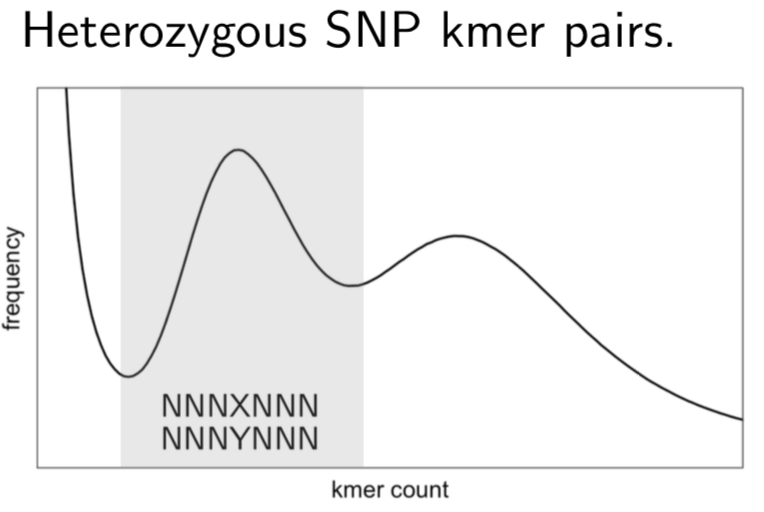
\includegraphics[width=0.65\textwidth]{kmc.png}
\par{An example of kmer count spectra showing error kmers on the left, heterozygous kmers in the first peak and homozygous kmers in the next peak.}
\end{centering}
\end{figure}

\par{
We then use the heterozygous range of the kmer spectra with code from purge dups, a tool for removing sequences from assemblies when multiple haplotypes were assembled separately\cite{purgedups}. The kmers are then dumped in alphabetical order and we search for pairs of kmers which vary in only the middle base and fall into the heterozygous counts range. We give a further restriction that the sum of the counts of the kmers with the other two possible bases in the middle are not high as sequences with very high repeat count can produce, through sequencing error or mutations, two kmers in these counts range with the middle base altered. It should also be noted, that while I generally refer to these kmer pairs as heterozygous kmer pairs, they may also represent paralogous kmer pairs. We will use the phasing consistency of these kmer pairs with each other to determine if they are more likely to be from heterozygosity or paralogous sequences. Each produces a characteristic pattern in the kmer consistency counts.
}

\subsection{Read data kmer information}
\par{
We will use the kmers in the reads to determine if heterozygous paired kmers are phasing consistent with other paired kmers. So we go through the reads of each long range genetic information including HiC, PacBio, linked reads, and nanopore and store the position and ID of each paired kmer on the reads. We then store this on disk in a custom binary format for later use. Of note here is that the linked read technology may have multiple molecules per barcode whereas in other technologies, reads represent single physically linked molecules. Richard Durbin has developed a method to \textit{de novo} assign reads from barcodes to molecule groups using shared kmers across barcode sets to cluster reads into their molecules of origin. In this work, we choose not to use this as it is unpublished and not extensively tested. Instead, we use the distance on the assembly contigs to determine which reads came from which barcode. With the recommended DNA input, high molecular weight (HMW) extraction sizes, and number of partitions, we expect the poisson loading to result in a mean of roughly ten molecules per barcode. Because the total amount of DNA per partition is a small percentage of the total genome sizes we work with, the chances of a partition having molecules which arose from nearby or overlapping locations is rare. Thus we can deduce that reads from a barcode which map close to one another on a reference or assembly arose from the same HMW molecule. While this is not fully \textit{de novo}, it is highly unlikely to cause a false inference because a chimeric misassembly causing incorrect linked read molecule inference would not result in a phasing consistent signal.
}

\begin{figure}[htbp!]

\caption{Identify paired kmer location in long range genetic data}
\label{figure:techs}
\begin{centering}
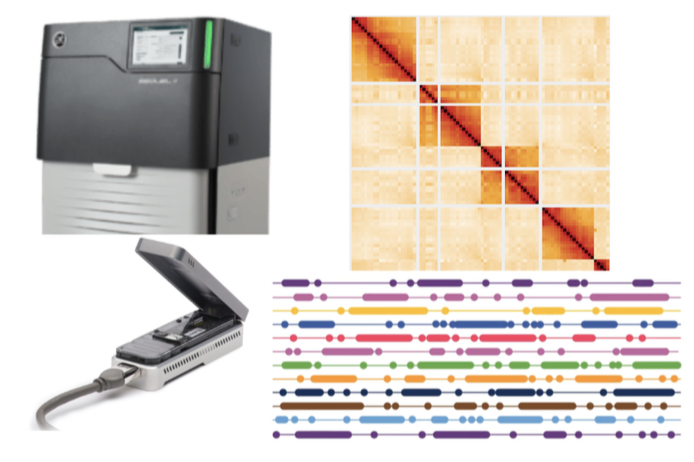
\includegraphics[width=0.65\textwidth]{techs.png}
\par{Different data types used. Top left: PacBio, Top right: Hi-C, Bottom left: nanopore, Bottom right: Linked reads}
\end{centering}
\end{figure}

\subsection{Pairwise haplotype phasing consistency}
\par{
For each kmer pair, we refer to one as the reference allele and one as the alternate allele arbitrarily without loss of generality. 
}


\begin{figure}[htbp!]
\caption{Pairwise phasing consistency counts}\label{figure:consistency}
\centering
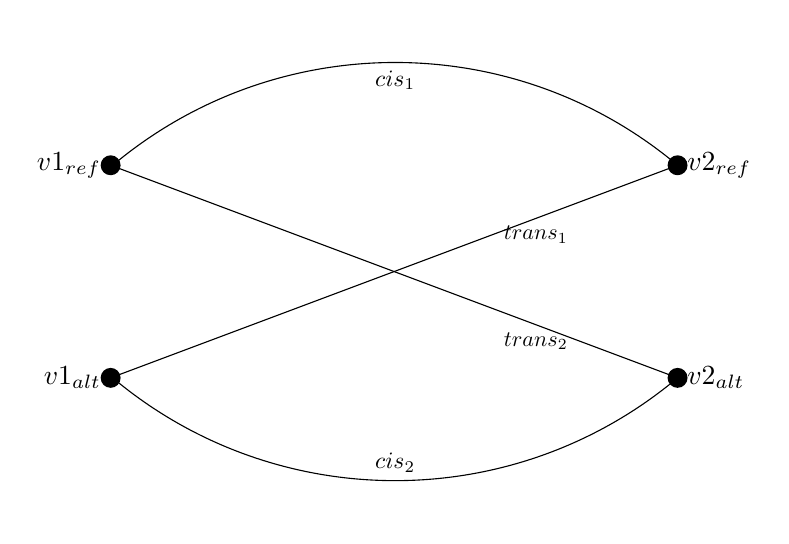
\begin{tikzpicture}[scale=1.8]
\def\xoffset{0}
\def\yoffset{0}
\def\titley{1.2}
\def\panellength{5}
\def\titlescale{1}
 \def\subtitlescale{0.7}
 \node[anchor=east] at (0 + \xoffset,2 + \yoffset) {$v1_{alt}$};
\draw (4 + \xoffset,2 + \yoffset) arc (-50:-130:3.1) node[midway,above, scale=0.85] {$cis_2$};
\fill (0 + \xoffset ,2 + \yoffset) circle[radius=2pt];
\node[anchor=west] at (4 + \xoffset,2 + \yoffset) {$v2_{alt}$};
\fill (4 + \xoffset,2 + \yoffset) circle[radius=2pt];
\node[anchor=east] at (0 + \xoffset,3.5 + \yoffset) {$v1_{ref}$};
\fill (0 + \xoffset,3.5 + \yoffset) circle[radius=2pt];
\draw (4 + \xoffset,3.5 + \yoffset) arc (50:130:3.1) node[midway,below, scale=0.85]{$cis_1$};
\draw (4 + \xoffset ,3.5 + \yoffset) -- node[below, scale=0.8] {$trans_1$} (2 + \xoffset,2.75 + \yoffset) -- (0+ \xoffset,2 + \yoffset);
\draw (4 + \xoffset,2 + \yoffset) -- node[below, scale=0.8] {$trans_2$} (2+ \xoffset,2.75 + \yoffset) -- (0+ \xoffset,3.5 + \yoffset);
\node[anchor=west] at (4+ \xoffset,3.5 + \yoffset) {$v2_{ref}$};
\fill (4+ \xoffset,3.5 + \yoffset) circle[radius=2pt];
\end{tikzpicture}
\par{
We denote one of each kmer pair as the reference or alternative arbitrarily. Molecules that have the sequences of one of the kmers from each of two kmer pairs will fall into one of four cases represented here by the four edges in this graph. We calculate the counts of molecules falling into each of these four categories. Phasing consistent heterozygous kmer pairs will have counts predominantly on both cis edges or both trans edges.
}
\end{figure}

\subsection{Multiple heterozygous site haplotype phasing consistency}



\subsection{de novo haplotype phasing}

\subsubsection{Sparse \textit{Bernoulli} mixture model clustering}


\cite{HICphasing} %place this somewhere





\section{Pedigree sample strategies}
As discussed already there are simple strategies for splitting long reads by haplotypes using short accurate reads from both parents. 
But for many species such as wild caught samples it may be difficult to obtain the paternal sample whereas it is possible to capture a 
fertilized female and grow her brood in isolation. For this case we propose to use three short read samples: one maternal sample, one sample 
from a single F1, and another sample from a pool of multiple F1 offspring. From these samples we can obtain distinguishing kmers or probabilistic 
distinguishing kmers for each haplotype of both the mother and father.

\begin{figure}[h!]
\caption{Pseudotrio}
\label{figure:pseudotrio}
\begin{centering}
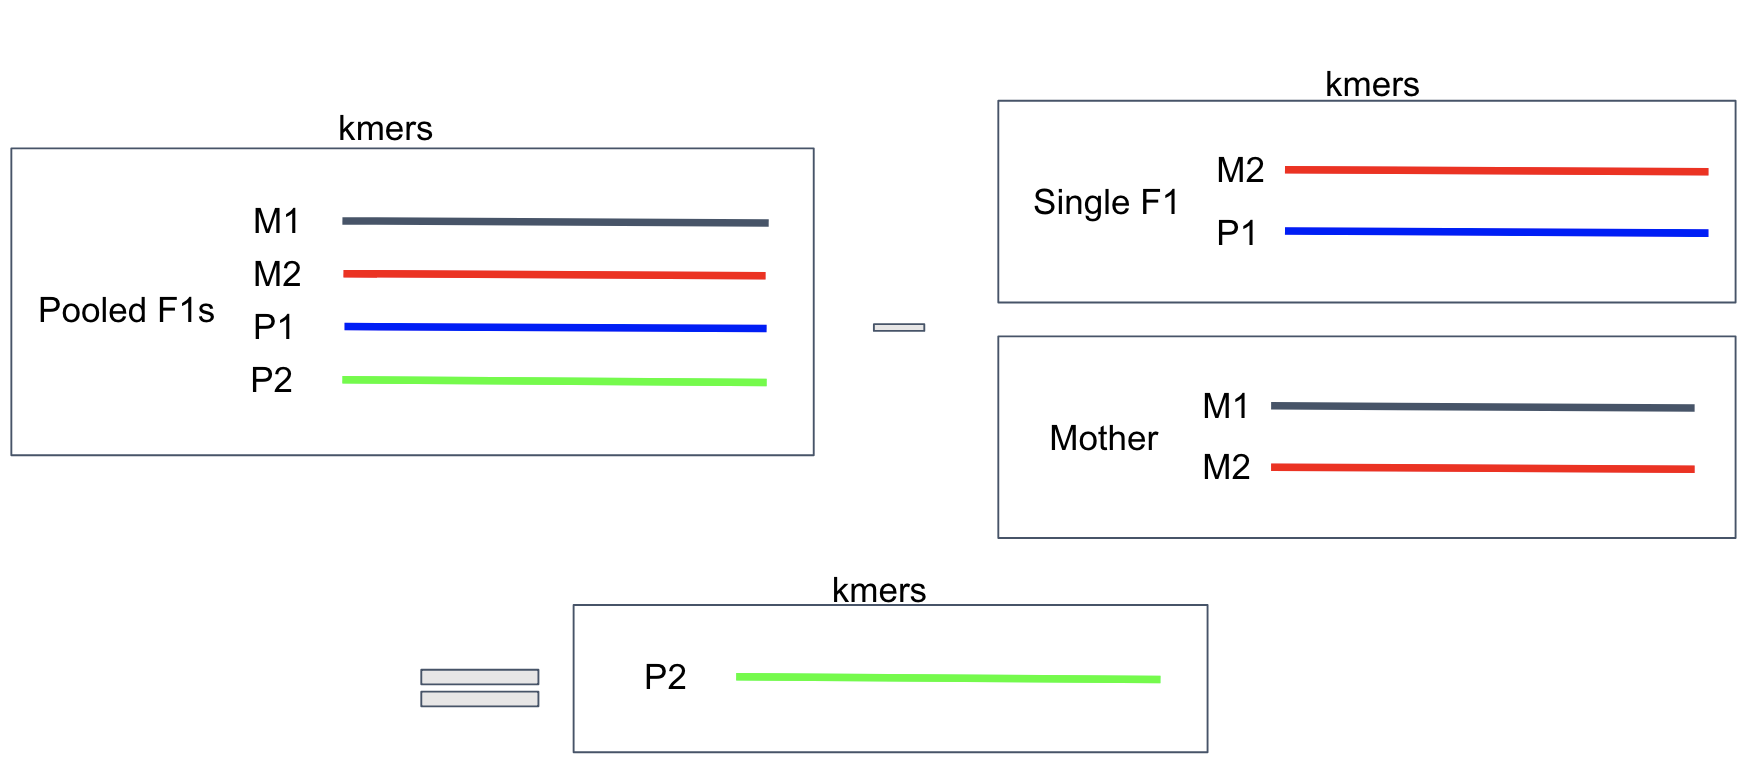
\includegraphics[width=\textwidth]{pseudotrio.png}
\end{centering}
\end{figure}

As shown in \ref{figure:pseudotrio} we can obtain distinguishing kmers for the P1 haplotype by set subtraction of kmers in the maternal and single F1 sample 
from the those in the pooled samples. In a similar way we can subtract kmers in the maternal sample from the single F1 sample to get probabilistic distinguishing 
kmers from the P2 haplotype. We say probabilistic distinguishing kmers because these kmers could also occur on the P1 haplotype as well. And in the same way 
we can get probabilistic distinguishing kmers for the M1 haplotype by subtracting kmers in the single F1 sample from those in the maternal sample. And finally we can obtain 
probabilistic distinguishing kmers for the M2 haplotype will be obtained by selecting kmers which are shared between the maternal and single F1 sample and occur at 
haploid counts in both samples. Once we have these distinguishing kmers we can use them to separate long reads by haplotype for libraries created from any of these samples. 
We have created software for collecting these distinguishing kmers \cite{distinguishing_kmers} which uses counting bloom filters to minimize memory usage 
and a mod based system allowing distribution of jobs to many worker nodes. And we also have software for binning long reads based on those 
distinguishing kmers \cite{long_read_binner}.


\section{Phasstools: phasing and assembly tools}
\subsection{Heterozygous kmer pairs and detection}
First we tackle the subject of identifying heterozygous variants in a reference-free manner. We will do this using a kmer approach, as many reference-free methods do. 
Many people have focused on identifying kmers which occur at roughly half counts in short read data \cite{KAT} and various software exists to count kmers \cite{jellyfish} 
and to model the mixture of expected distributions (errors, haploid, diploid, duplication kmers) \cite{genomescope}. Identifying heterozygous kmers in this way 
suffers from multiple problems from the perspective of de novo phasing. 1. Many of these identified as half counts will be either randomly high count error kmers or randomly low count 
homozygous kmers. 2. You end up with $K-1$ overlapping kmers for a given variant which is needlessly redundant information which will both slow down any phasing algorithm and 
likely break key independence assumptions. And 3. while you have heterozygous kmers, you don't know which kmers are alternative alleles of each other. 
We propose finding pairs of kmers which vary only in the center position which are also both roughly at half counts. These heterozgyous SNP kmers 
will be much more robust and have the benefit of knowing that one is the alternative allele of the other.
We have software for this purpose \cite{het_kmers} which uses counting bloom filters to minimize memory usage and a mod based method to 
distribute the work to many worker nodes.

\subsection{Phasing consistency}

\subsection{Data types and uses}


\subsection{Phasst phase: Reference or assembly based phasing}
\subsubsection{Sparse \textit{Bernoulli} mixture model clustering}
\subsubsection{Polyploid phasing}
\subsubsection{Phasing consistency genotype correction}
\subsection{Phasst a: phased assembly}
\subsubsection{Phasing consistent heterozygous kmer recruitment}
\subsubsection{Haplotype and chromosome read binning}
\subsubsection{Haploid chromosome assemly}
\subsection{Phasst scaff: phasing aware assembly scaffolding}
\subsubsection{Chromosome binning}
\subsubsection{Ordering and Orienting}


%\section{De novo haplotype phasing}
In order to separate long reads by haplotype for a single individual, we must develop an algorithm for de novo haplotype phasing. In reference based systems, haplotype 
phasing begins by mapping reads to the reference and calling variants from the reference. Then physical linkage information of two heterozygous variants occurring 
on data known to be generated from a single haplotype is used to determine which alleles come from which of the sister chromosomes across 
either some region (denoted as a phase block) or 
across whole chromosomes \cite{10xlinked} \cite{whatshap} \cite{hapcut2} \cite{hapchat}. At each heterozygous variant locus, one allele can arbitrarily be denoted as 0 and 
the second allele denoted 1. Then without loss of generality we choose to represent the series of alleles located on whichever chromosome has the 0 allele of the first variant in 
a phase block. So now the problem can be seen as determining the binary sequence of which alleles are on that same chromosome that are most consistent 
with the linkage data we have. To do this, each of these methods uses different search strategies (beam search, dynamic programming, graph based heuristic search) to find the 
configuration that maximizes the probability of the data under some error model. These algorithms are also aided by the knowledge of which variants are close to each other (and 
thus are most likely to contain linkage information) on the genome. It is common to proceed in a directed manner, determining the optimal solution for variants $[0..n-1]$ before 
determining the phase of variant $n$. So for de novo haplotype phasing we will need to 1. identify heterozygous alleles 2. determine an ordering of those alleles and 3. create a 
search strategy to maximize a probabilistic model of the data. 



\subsubsection{Diploid assembly validation}

While certain tools for assembly validation are available \cite{KAT} \cite{busco}, the validation of diploid assemblies is a difficult problem still in its infancy. 
These heterozygous kmers are also useful for validating diploid assemblies because you expect to see one of the heterozygous kmer pairs in the primary assembly 
and the other one in the secondary haplotigs. If, for instance, you find both versions of a heterozygous kmer pair in the primary assembly, this could either represent residual 
heterozygosity in the primary assembly which should be removed, or perhaps the kmers came from paralogous regions and both kmers had lower than homozygous counts 
due to random sampling error. Another error type that exists is lacking either of the kmer pair in the primary which could represent low base level accuracy, over collapse of near repeat regions, or some other type of error. Other cases exist which may have their own interpretations. We have developed software for this analysis which is now in use by the Sanger 
assembly curation team \cite{haplovalidate}.

%\subsection{De novo phasing algorithm strategy}
The next step for de novo phasing is determining a rough ordering of heterozygous SNPs. If we view the heterozygous kmers as nodes in a graph and edges between 
nodes as linkage information of long reads or other long genetic distance linkage information with weights as the number of those links, we could view our problem as a 
graph based traveling salesman problem in which we want to find the maximum scoring traversal of nodes in which each node is only visited once. While the traveling salesman 
problem is known to be an NP-hard problem, greedy approximation algorithms exist with fast implementations \cite{randomwalkTSP}, and we don't need the true optimal ordering. 
We just need an ordering such that heterozygous SNPs near one another in the ordering are likely to share linkage information in our data.

Once we have a pseudo ordering of heterozygous SNP kmers, we could proceed in many different ways including methods which already exist \cite{10xlinked}. 
Or we could approach the problem from a novel angle with some benefits. We propose to solve the haplotype phasing search problem with mixture model clustering. In this case, 
each cluster center would be a vector of length $n$ where $n$ is the number of heterozgyous kmers in some chunk which we believe should share linkage and the values in that 
vector would represent the allele fraction on that haplotype of one of the alleles chosen arbitrarily. When optimized, these values would tend toward 0 and 1 assuming the data 
supports a diploid structure.  Similar to our single cell genotype clustering algorithm, we marginalize each read 
across the possible haplotypes. Then the negative log likelihood should be differentiable and susceptible to numerical optimization techniques. This method has several potential 
advantages over current approximation search algorithms. One is that is is trivially extendable to polyploid genomes. In the polyploid case, the only thing that changes is that there are $P = ploidy$ cluster centers instead of just two. Another benefit is that it can handle cases in which one of the variants chosen is not actually heterozygous but is homozygous for one 
of the alleles. Including these cases can dramatically slow down current algorithms, but is beneficial in error correcting variant calls \cite{10xpatent}. This algorithm could also be used 
in reference based systems.

\section{Discussion}


%!TEX root = ../thesis.tex
%\input{commands.tex}
%*******************************************************************************
%****************************** Third Chapter **********************************
%*******************************************************************************
\chapter{Conclusions}

% **************************** Define Graphics Path **************************
\ifpdf
    \graphicspath{{Chapter5/Figs/Raster/}{Chapter5/Figs/PDF/}{Chapter5/Figs/}}
\else
    \graphicspath{{Chapter5/Figs/Vector/}{Chapter5/Figs/}}
\fi


\par{
Genetic variation along with natural selection, has driven the evolutionary history on earth creating us and all other life we know. Much work has been done to assess the population variation across humans and other species and use that to link genotypes with phenotypes and infer evolutionary histories. Less work has used these as markers to disambiguate data in different problems in genomics.
}
\par{
Single cell RNAseq suffers from several error modes that arise from natural limitations of detections of small materials as well as from the strategy used to partition cells. Because cells contain miniscule amounts of mRNA, amplification methods must be used which incur technical artifacts between cells within an experiment and more across experiments. Because cells are loaded into droplets in a poisson process, in order to capture many singletons, the cell suspension must be in a concentration that will also randomly load two or more cells into a single droplet. And if cells lyse or if there is RNA in solution prior to partitioning, some reads will have cell barcodes of cells from which they did not originate. One experimental design promises to address each of these issues at once. Mixing cells from multiple individuals reduces the batch effects when comparing them, cross sample multiplets should be easier to identify and remove, and the skew in allele fractions away from those expected from a diploid genome may be used to measure the ambient RNA. In chapter 2, I presented souporcell, a computational tool which uses the genetic variation between individuals to cluster cells in a single cell RNAseq mixture of individuals by the variants expressed in the reads. Souporcell also calls doublets using the alleles in cells versus the alleles in each cluster. And souporcell estimates the amount of ambient RNA in the system by how far the allele fractions in the clusters vary from those one expects from a diploid organism. I validated and compared souporcell to the other relevant tools and found that it compared favorably against all of them including the previous gold standard, demuxlet, which requires more information \textit{a priori}. I believe this is due to the rigid model based system used in demuxlet versus the simple cluster center method which is robust to any unmodeled factors. Souporcell has already been used in several million+ cell experiments and has been externally validated using cell hashing. I believe that mixture experimental designs will only get more popular over time due to the advantages this strategy has. 
}

\par{
Long read sequencing has undoubtedly revolutionized genome assembly and has motivated large projects such as the Darwin Tree of Life and the Earth Biogenome project which seek to sequence and assemble quality genomes for all multicellular eukaryotic organisms. This will provide the next generation of science with an invaluable resource, allow for insights into evolution not before possible, and serve as a conservation of biological information in an era of extinction unprecedented during humans' time on earth. While much progress has been made through both data improvements and algorithmic methods, some issues remain especially for small organisms and highly heterozygous genomes. In chapter 3, we present the first high quality assembly of a single mosquito. This was made possible by recent advances in library preparation for long read sequencing reducing the DNA requirements. This improved the assembly versus other mosquito assemblies which used pools of individuals or short reads because of the presence of only two haplotypes versus many haplotypes.
}

\par{
While many consider heterozygosity a hinderance to genome assembly, and most assemblers perform worse on highly heterozygous genomes, it can have some benefits as well. In chapter 4, I turn this idea that heterozygosity is bad on its head and instead use heterozygosity as an advantage by using the phasing consistency of reads across multiple heterozygous sites as a signal for physical linkage in both assembly and scaffolding. In doing this, I also describe two phasing algorithms (three, if phased assembly is counted). One of these algorithms is novel and has several benefits of general interest. It is both robust to, and can correct incorrect genotypes because it does not make the assumption that every input variant is heterozygous and has relaxed the discrete constraint shared by most phasing algorithms. Another benefit of this algorithm is that it scales well for polyploid because we use treat haplotypes as cluster centers and can trivially increase the number of clusters as the ploidy increases. We demonstrate our phased assembly and scaffolding on the lepidoptera \textit{Vanessa atalanta}. While we do not meet the contiguity of some modern assemblers and do not assemble sex chromosomes, these can be assembled separately. We believe that phased assembly is the correct solution to diploid and polyploid assembly.
}
%\include{Chapter6/chapter6}
%\include{Chapter7/chapter7}



% ********************************** Back Matter *******************************
% Backmatter should be commented out, if you are using appendices after References
\backmatter

% ********************************** Bibliography ******************************
\begin{spacing}{0.9}

% To use the conventional natbib style referencing
% Bibliography style previews: http://nodonn.tipido.net/bibstyle.php
% Reference styles: http://sites.stat.psu.edu/~surajit/present/bib.htm

%\bibliographystyle{apalike}
%\bibliographystyle{unsrt} % Use for unsorted references  
\bibliographystyle{plainnat} % use this to have URLs listed in References
\cleardoublepage
\bibliography{References/references} % Path to your References.bib file


% If you would like to use BibLaTeX for your references, pass `custombib' as
% an option in the document class. The location of 'reference.bib' should be
% specified in the preamble.tex file in the custombib section.
% Comment out the lines related to natbib above and uncomment the following line.

%\printbibliography[heading=bibintoc, title={References}]


\end{spacing}

% ********************************** Appendices ********************************

\begin{appendices} % Using appendices environment for more functunality

%%!TEX root = ../thesis.tex
% ******************************* Thesis Appendix A ****************************
\chapter{Related publications}

During my graduate studies I have been an author on a number of publications which are related to this work.
These include the following:

\begin{itemize}[noitemsep]

\item Garrison, Erik, Jouni Sirén, Adam M. Novak, Glenn Hickey, Jordan M. Eizenga, Eric T. Dawson, William Jones et al. ``Variation graph toolkit improves read mapping by representing genetic variation in the reference.'' \emph{Nature biotechnology}, 36(9):875--879, (2018).

\item Paten, Benedict, Jordan M. Eizenga, Yohei M. Rosen, Adam M. Novak, Erik Garrison, and Glenn Hickey. ``Superbubbles, ultrabubbles, and cacti.'' \emph{Journal of Computational Biology}, 25(7):649--663, (2018).

\item Garg, Shilpa, Mikko Rautiainen, Adam M. Novak, Erik Garrison, Richard Durbin, and Tobias Marschall. ``A graph-based approach to diploid genome assembly.'' \emph{Bioinformatics}, 34(13):i105--i114, (2018).

\item Sirén, Jouni, Erik Garrison, Adam M. Novak, Benedict Paten, and Richard Durbin. ``Haplotype-aware graph indexes.'' \emph{arXiv:1805.03834} (2018).

\item Paten, Benedict, Adam M. Novak, Jordan M. Eizenga, and Erik Garrison. ``Genome graphs and the evolution of genome inference.'' \emph{Genome Research}, 27(5):665--676, (2017).

\item Novak, Adam M., Glenn Hickey, Erik Garrison, Sean Blum, Abram Connelly, Alexander Dilthey, Jordan Eizenga et al. ``Genome graphs.'' \emph{bioRxiv:101378} (2017).

\item Computational pan-genomics consortium. ``Computational pan-genomics: status, promises and challenges.'' \emph{Briefings in Bioinformatics}, 19(1):118--135, (2016).

\item Novak, Adam M., Erik Garrison, and Benedict Paten. ``A graph extension of the positional Burrows–Wheeler transform and its applications.'' \emph{Algorithms for Molecular Biology}, 12:18, (2017).

\end{itemize}

%%!TEX root = ../thesis.tex
% ******************************* Thesis Appendix B ********************************

\chapter{Installing the CUED class file}

\LaTeX.cls files can be accessed system-wide when they are placed in the
<texmf>/tex/latex directory, where <texmf> is the root directory of the user’s \TeX installation. On systems that have a local texmf tree (<texmflocal>), which
may be named ``texmf-local'' or ``localtexmf'', it may be advisable to install packages in <texmflocal>, rather than <texmf> as the contents of the former, unlike that of the latter, are preserved after the \LaTeX system is reinstalled and/or upgraded.

It is recommended that the user create a subdirectory <texmf>/tex/latex/CUED for all CUED related \LaTeX class and package files. On some \LaTeX systems, the directory look-up tables will need to be refreshed after making additions or deletions to the system files. For \TeX Live systems this is accomplished via executing ``texhash'' as root. MIK\TeX users can run ``initexmf -u'' to accomplish the same thing.

Users not willing or able to install the files system-wide can install them in their personal directories, but will then have to provide the path (full or relative) in addition to the filename when referring to them in \LaTeX.



\end{appendices}

% *************************************** Index ********************************
\printthesisindex % If index is present

\end{document}
